

%---------------------------------------
\subsection{Simulation MAS}
%---------------------------------------


Pour tester la machine virtuelle crée, les paramètres suivantes ont étés adoptées : $p=2; Rs = 3m\Omega; Rr=4.5m\Omega; Ls=210uH; L_r = L_s; M_{sr}=195.5uH; f=1.1 \cdot 10^{-3} kg\cdot m^2 \cdot s^{-1}; J = 10.8 \cdot 10^-3{kg \cdot m^2}$. Aussi, avec ces paramètres et définissant $\tau_i=\tau_{eq}$ et $K_p = 3 \cdot R_{eq}$, c'est possible calculer $\tau_i = 4.1\cdot 10^-3$ et $K_p = 2.07 \cdot 10^-2$.

Dans les simulations, une vitesse cible de \(1500 \frac{rad}{s}\) et des courants de référence de \(150 A\) pour le repère dq du stator ont été établis, isolant ainsi le contrôleur de vitesse pour une analyse plus nette. Cette configuration, choisie pour sa clarté dans l'analyse des données, utilise un intervalle de simulation de 30 secondes avec un simulateur discret à pas fixe de \(10^{-4}\) et un solveur de type Runge-Kutta d'ordre 4.

La courbe de vitesse angulaire du rotor montre une augmentation amortie jusqu'à stabiliser à \(1500 \frac{rad}{s}\), soit \(1.4324 \times 10^4 Hz\). Ce comportement démontre l'efficacité du système à atteindre la vitesse désirée, un aspect positif de la performance de la machine :

% ela poderia ir mais rápido ?

\begin{figure}[!h]
    \centering
    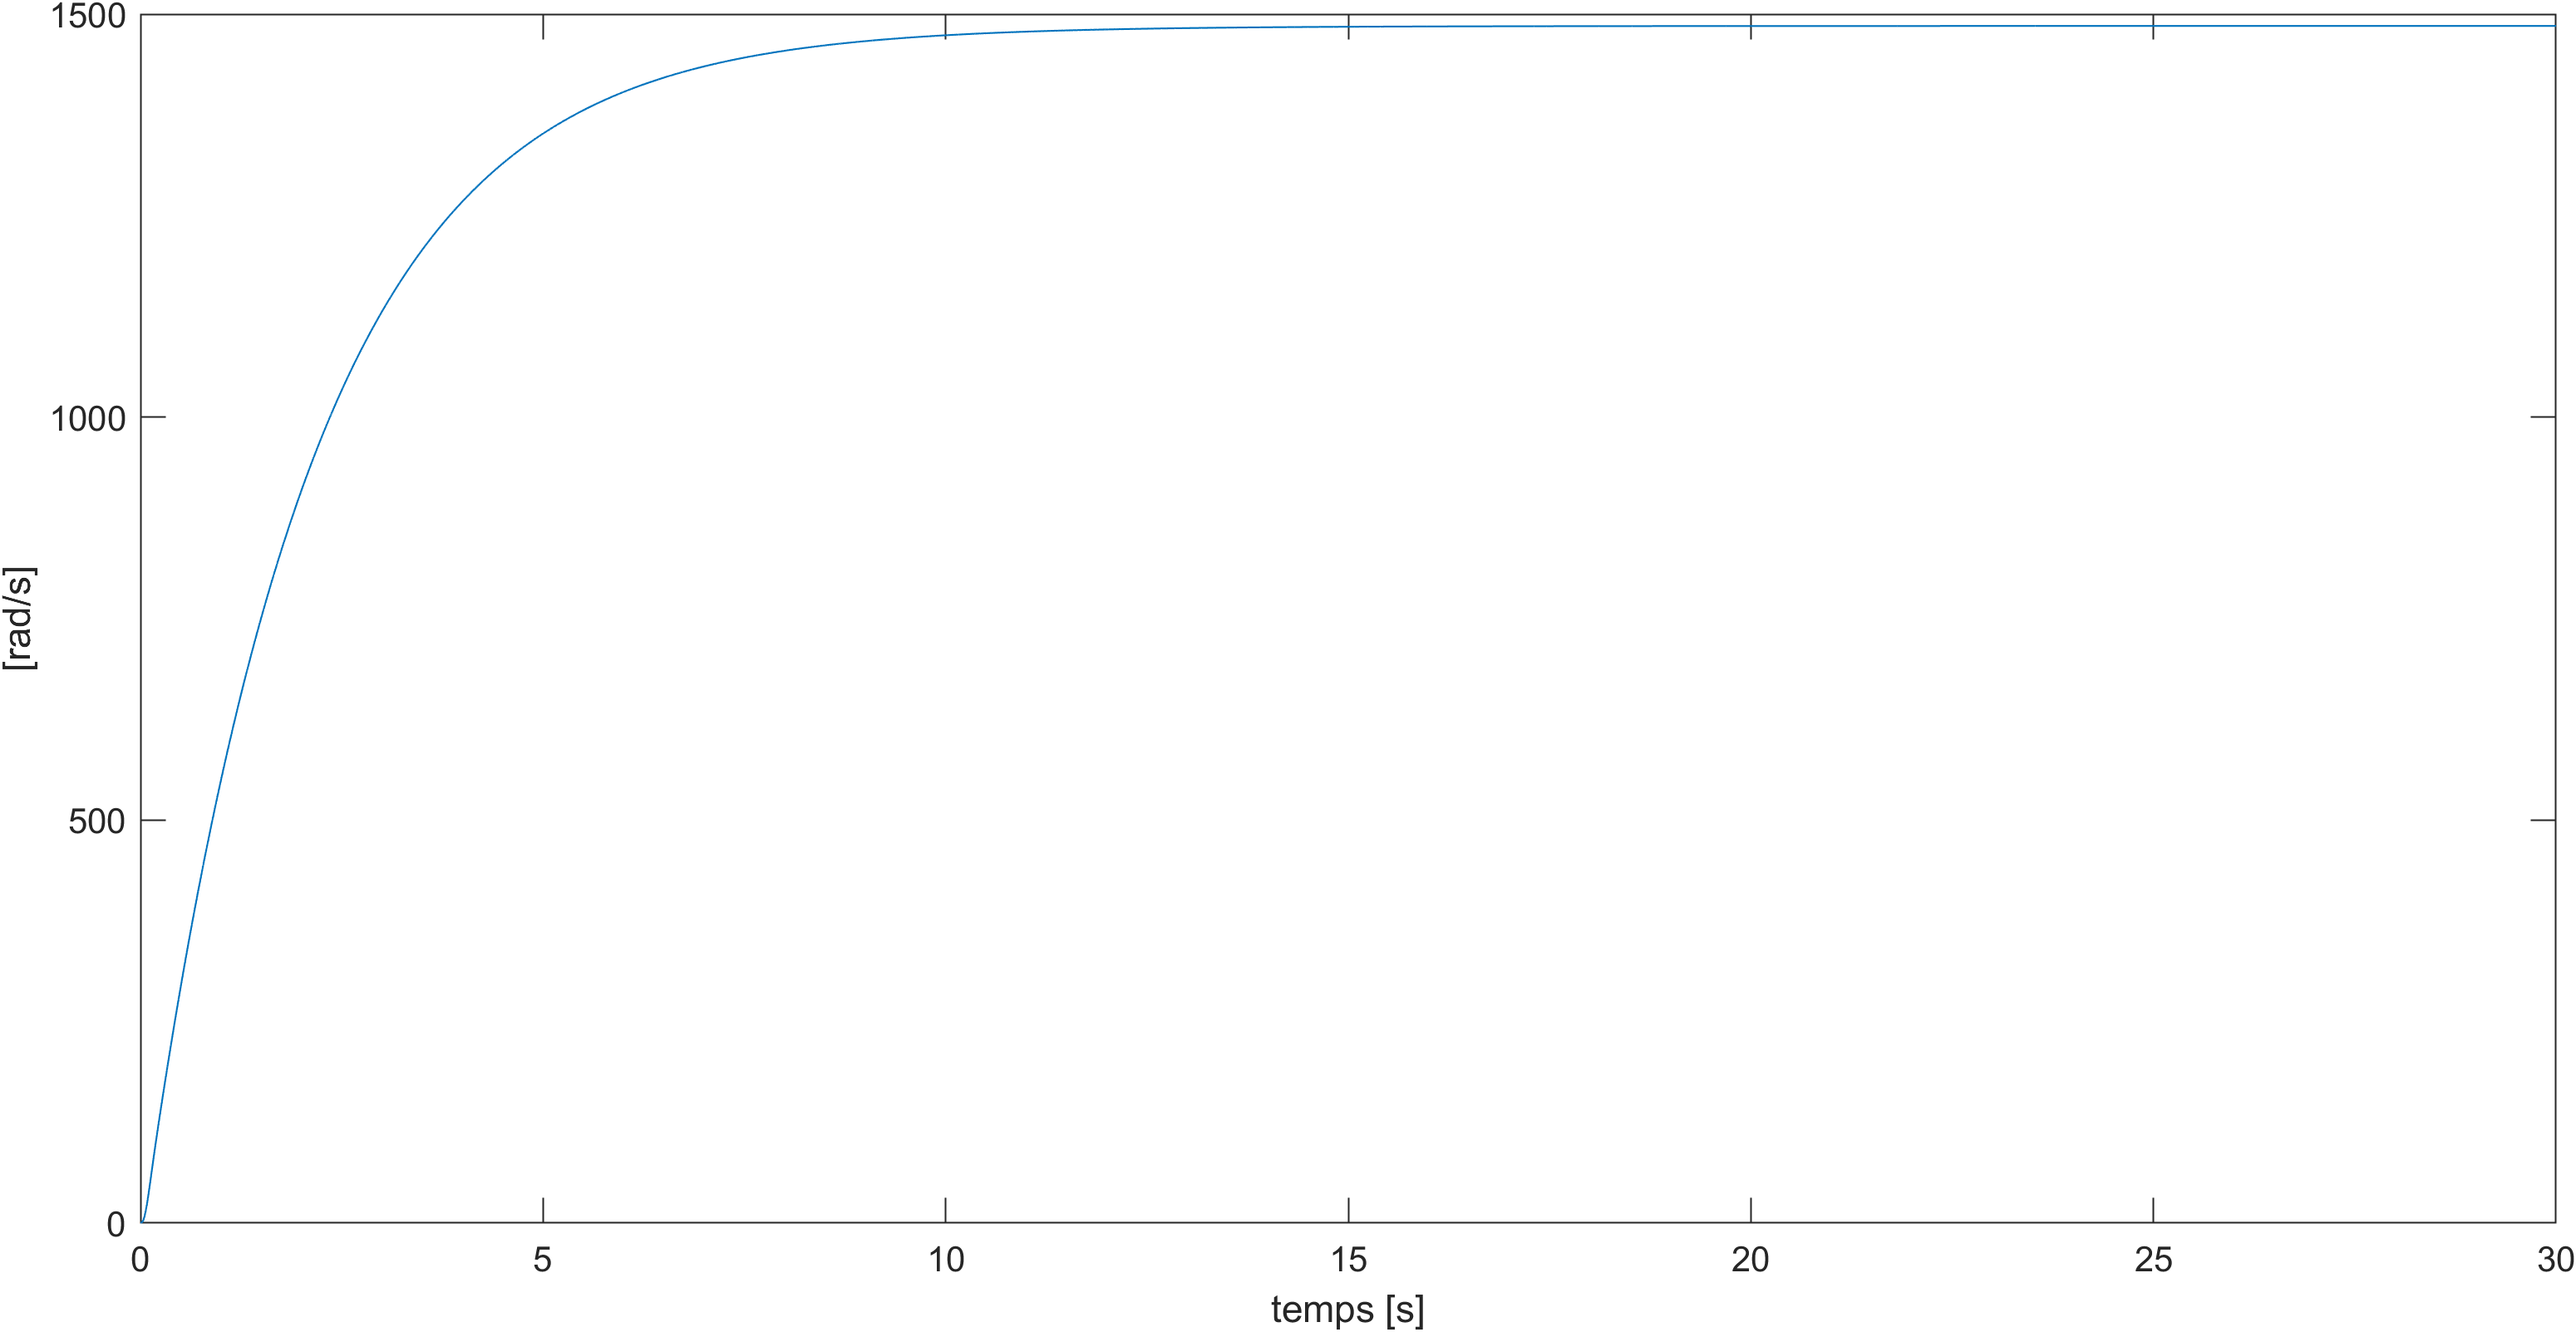
\includegraphics[width=0.8\textwidth]{simusMATLAB/MAS/wm.png} 
    \caption{Vitesse angulaire du rotor de la MAS mesurée au cours du temps.}
    \label{img-simuMatlab-wm}
\end{figure}

La Figure \ref{img-simuMatlab-is_abc} illustrant les courants triphasés dans le stator révèle une phase transitoire dans les premiers dixièmes de seconde, typique d'un démarrage. Passé ce moment, dès 0,2 seconde, les courants alternatifs commencent à converger, indiquant une stabilisation rapide du système sous l'effet du contrôleur.


\begin{figure}[!h]
    \centering
    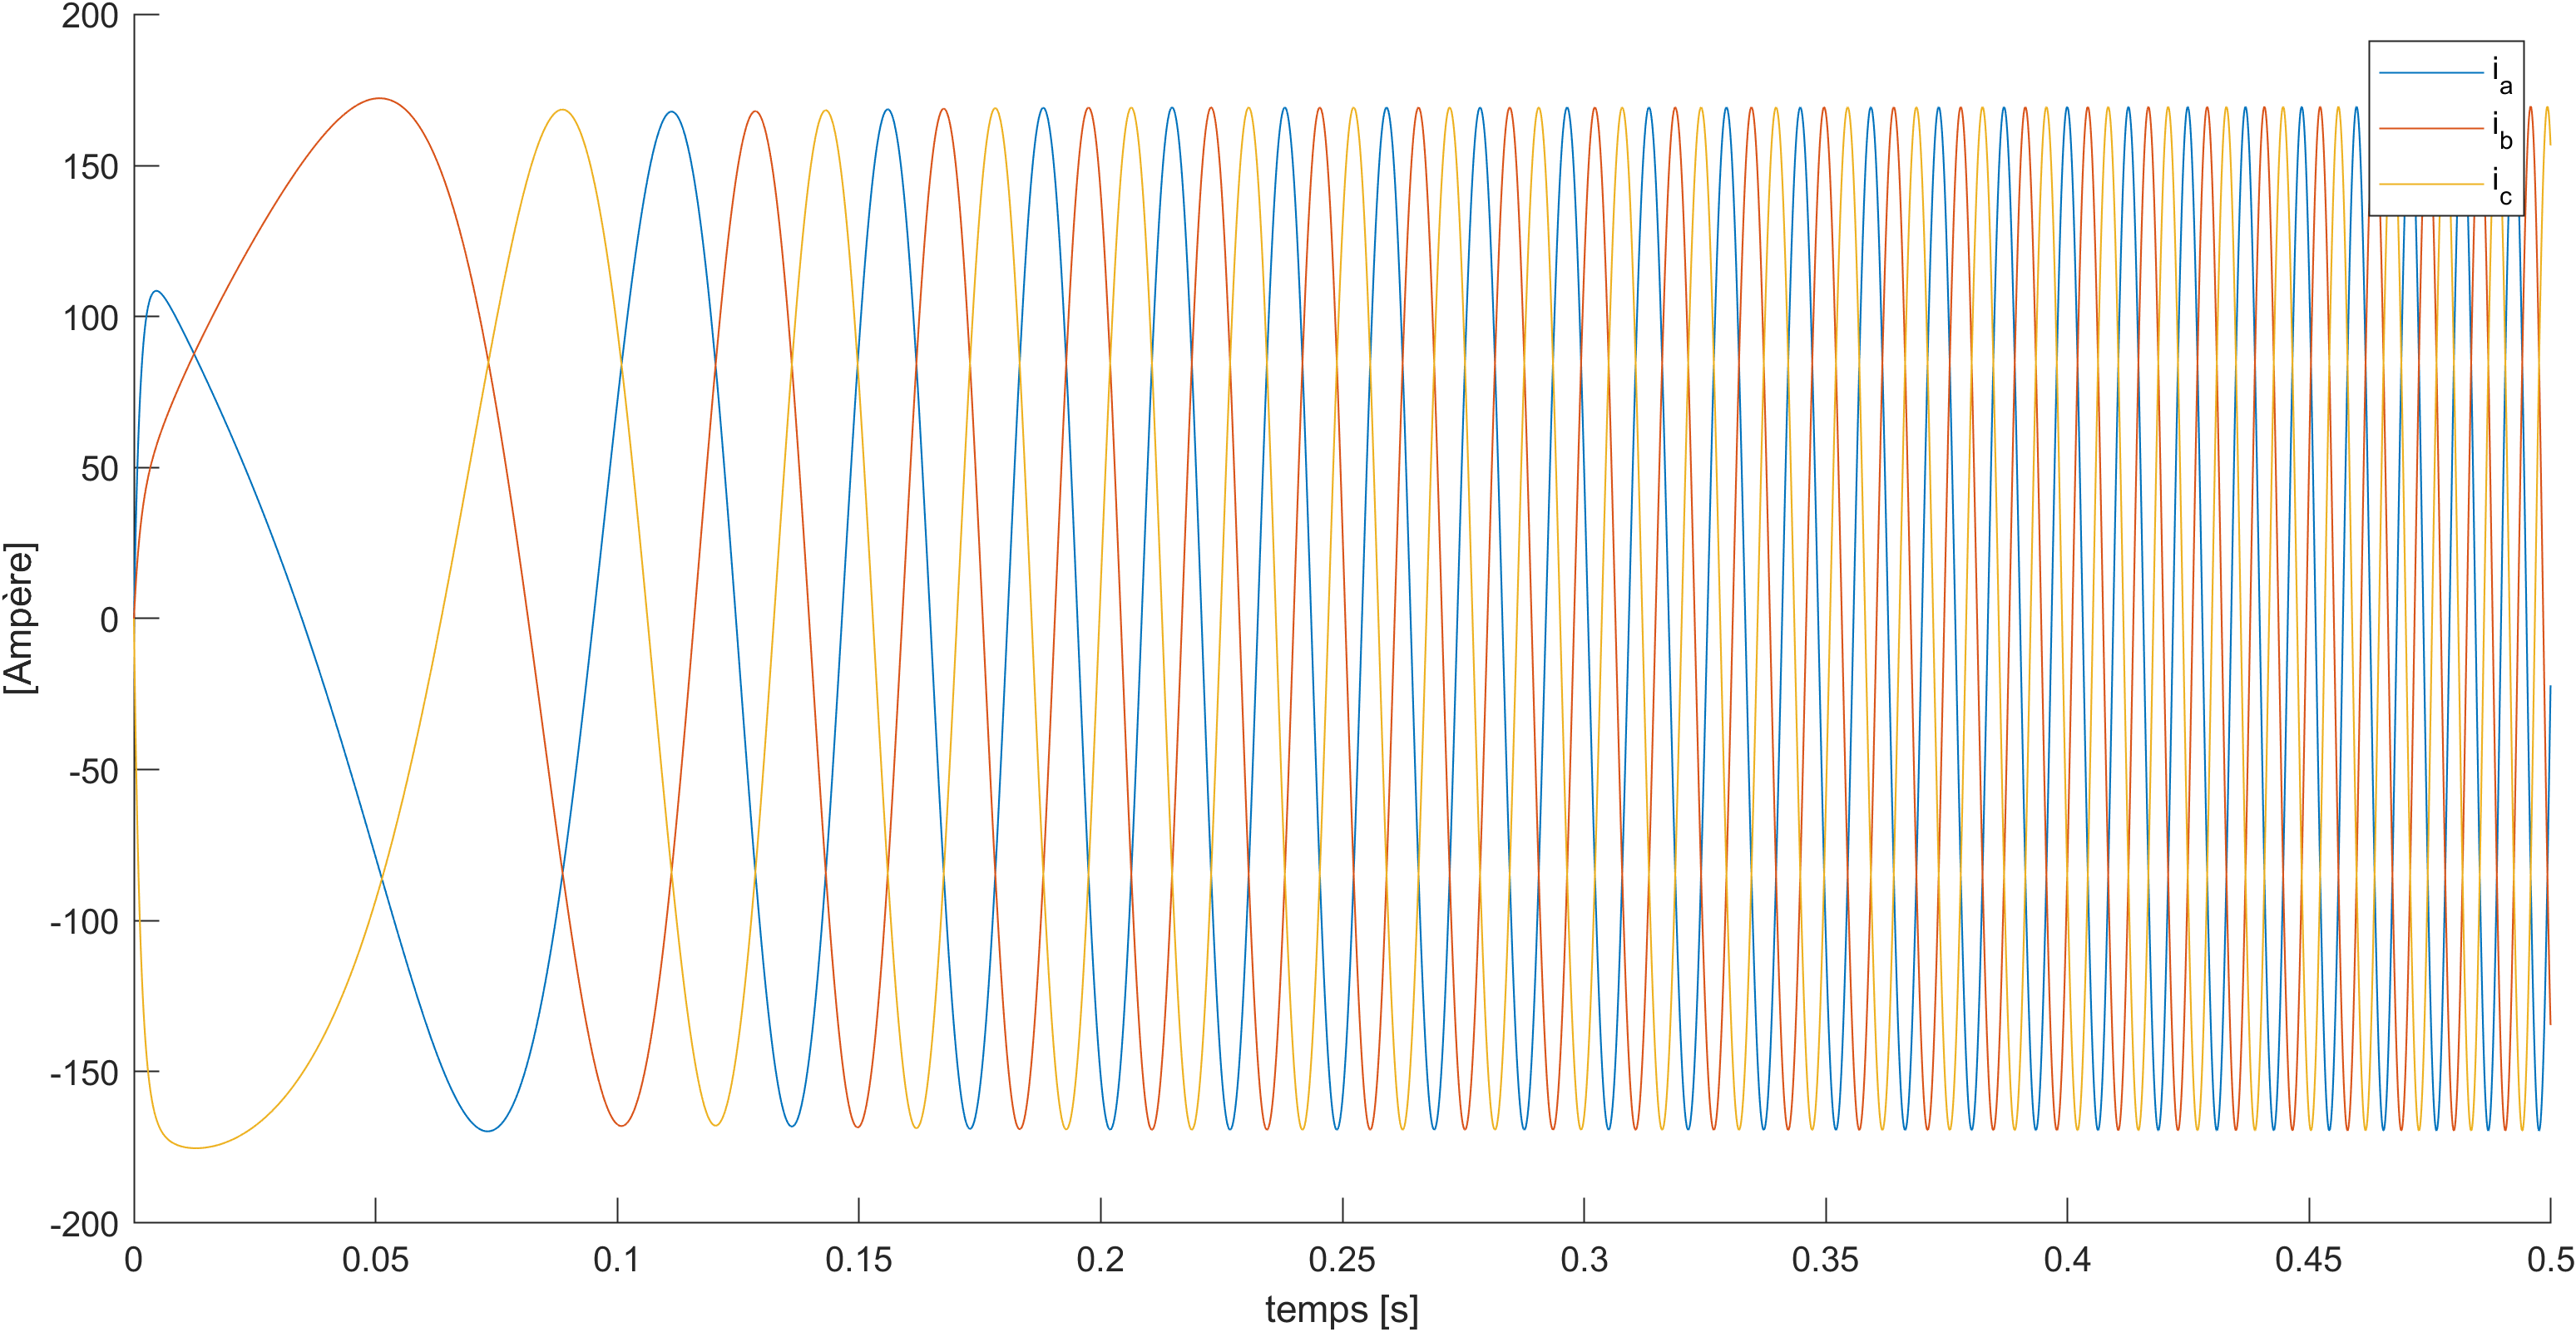
\includegraphics[width=0.8\textwidth]{simusMATLAB/MAS/is_abc.png} 
    \caption{Courants triphasées do stator de la MAS mesurées au cous du temps.}
    \label{img-simuMatlab-is_abc}
\end{figure}

Dans la Figure \ref{img-simuMatlab-is_dq}, un comportement transitoire initial évolue rapidement vers une stabilisation autour de la valeur cible de 150 A, illustrant l'efficacité du contrôle exercé sur le système :


\begin{figure}[!h]
    \centering
    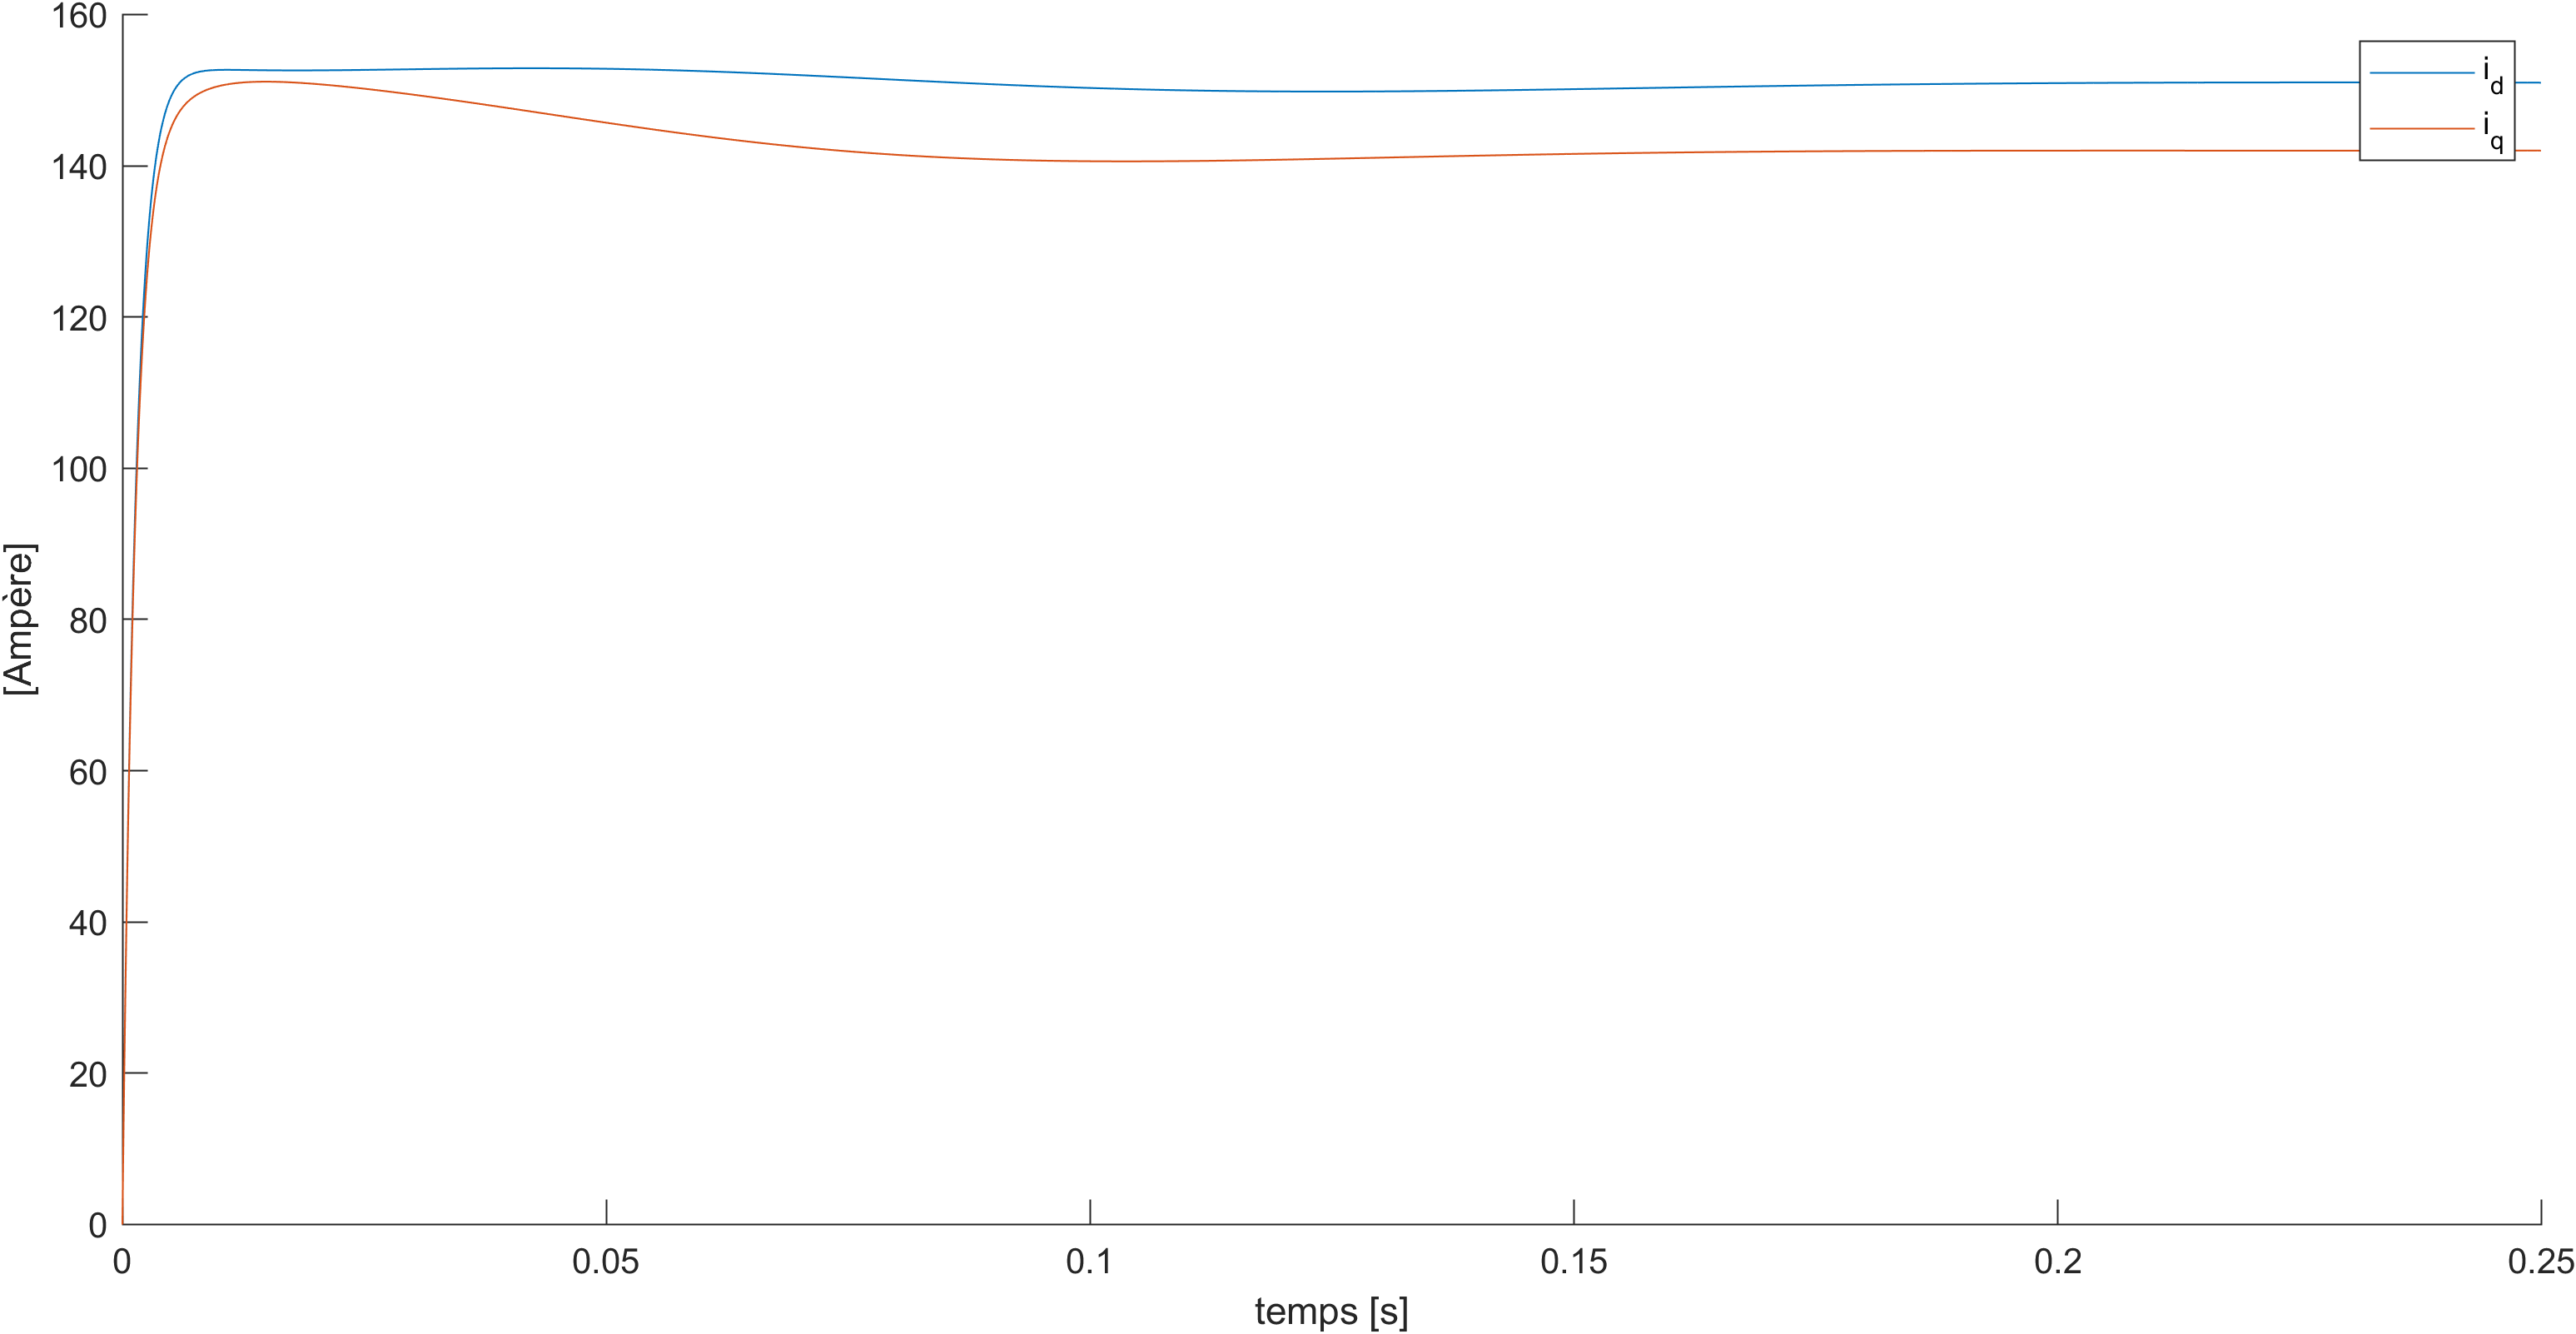
\includegraphics[width=0.8\textwidth]{simusMATLAB/MAS/is_dq.png} 
    \caption{Courants dans le repère dq du stator de la MAS au cous du temps.}
    \label{img-simuMatlab-is_dq}
\end{figure}


La comparaison entre les figures \ref{img-simuMatlab-is_dq} et \ref{img-simuMatlab-is_alphabeta} illustre efficacement la validité de la transformation de Park. Elle démontre visuellement comment les courants dans le repère dq sont affectés par la variation de fréquence \(\theta_s\), offrant une perspective claire sur la dynamique des courants sous cette transformation.


\begin{figure}[!h]
    \centering
    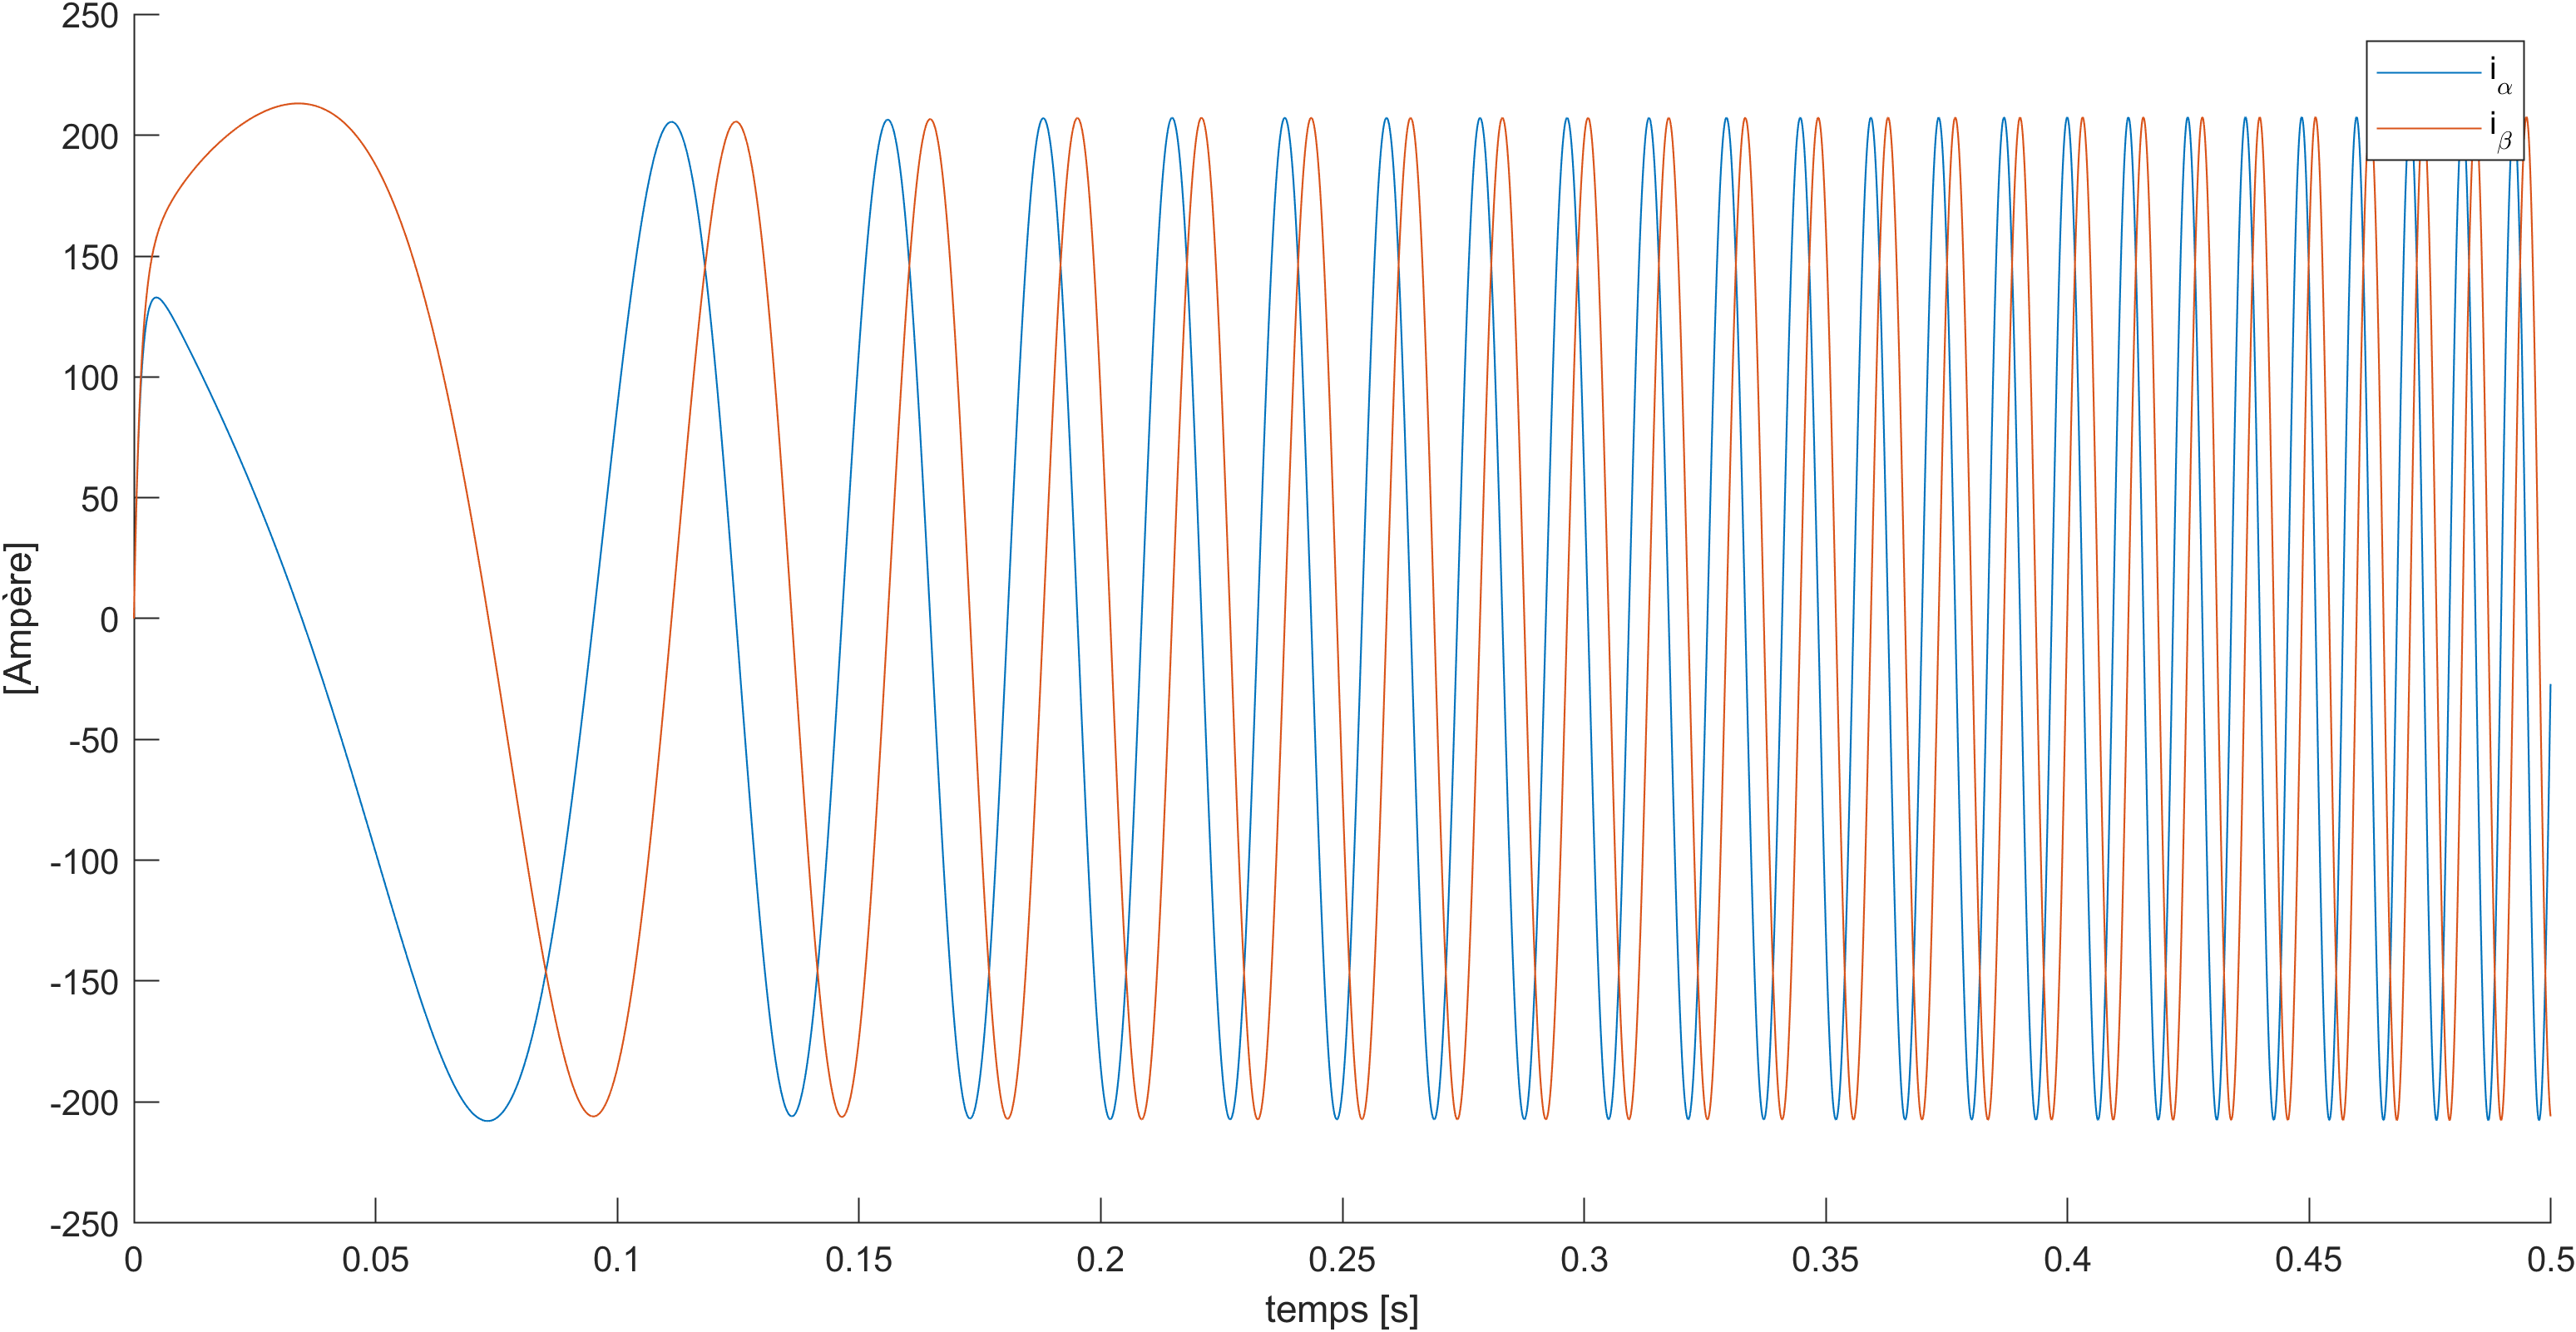
\includegraphics[width=0.8\textwidth]{simusMATLAB/MAS/is_alphabeta.png} 
    \caption{Courants dans le repère $\alpha\beta$ du stator de la machine au cous du temps.}
    \label{img-simuMatlab-is_alphabeta}
\end{figure}

L'analyse des données du stator de la machine asynchrone simulée révèle un comportement cohérent pour les tensions, similaire à celui observé pour les courants. La Figure \ref{img-simuMatlab-vs_abc} illustre les tensions triphasées, tandis que \ref{img-simuMatlab-Vs_dq} présente ces tensions dans le repère dq. La transformation de Park, appliquée en utilisant l'angle variable du stator, est validée par ces observations, comme le montre la Figure \ref{img-simuMatlab-Vs_alphabeta}, démontrant la conversion des tensions en suivant la fréquence de rotation \(\theta_s\).


\begin{figure}[!h]
    \centering
    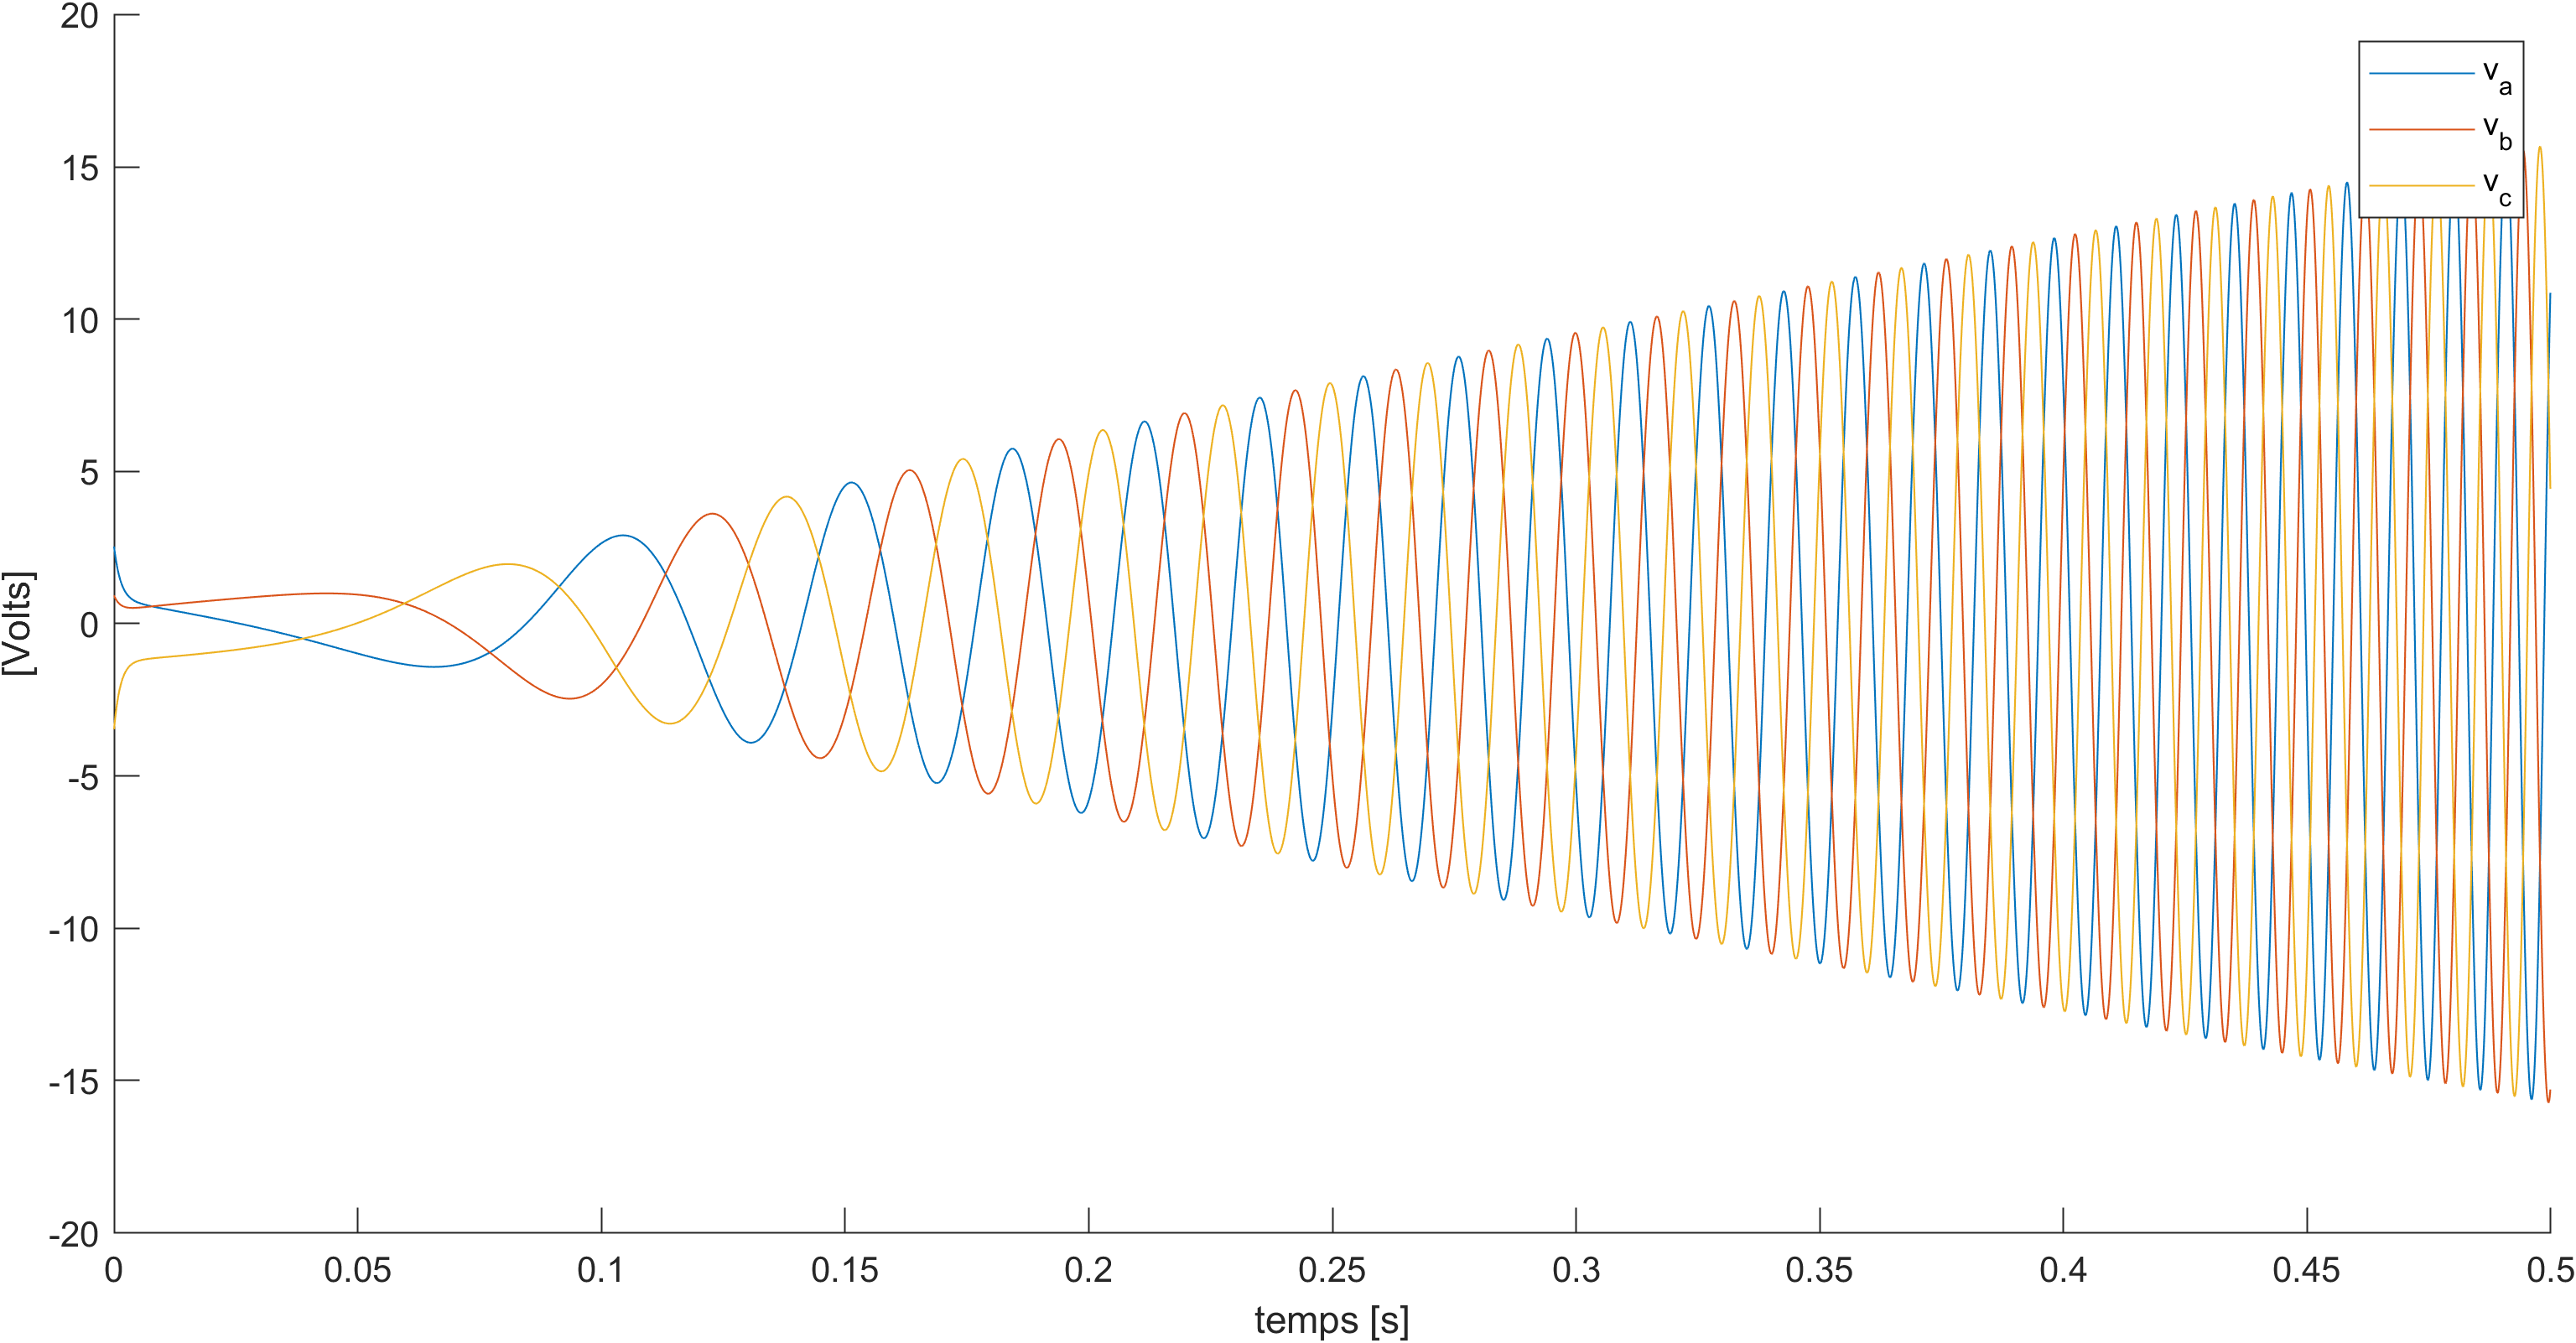
\includegraphics[width=0.8\textwidth]{simusMATLAB/MAS/vs_abc.png} 
    \caption{Tensions triphasées du stator de la MAS mesurées au cous du temps.}
    \label{img-simuMatlab-vs_abc}
\end{figure}

\begin{figure}[!h]
    \centering
    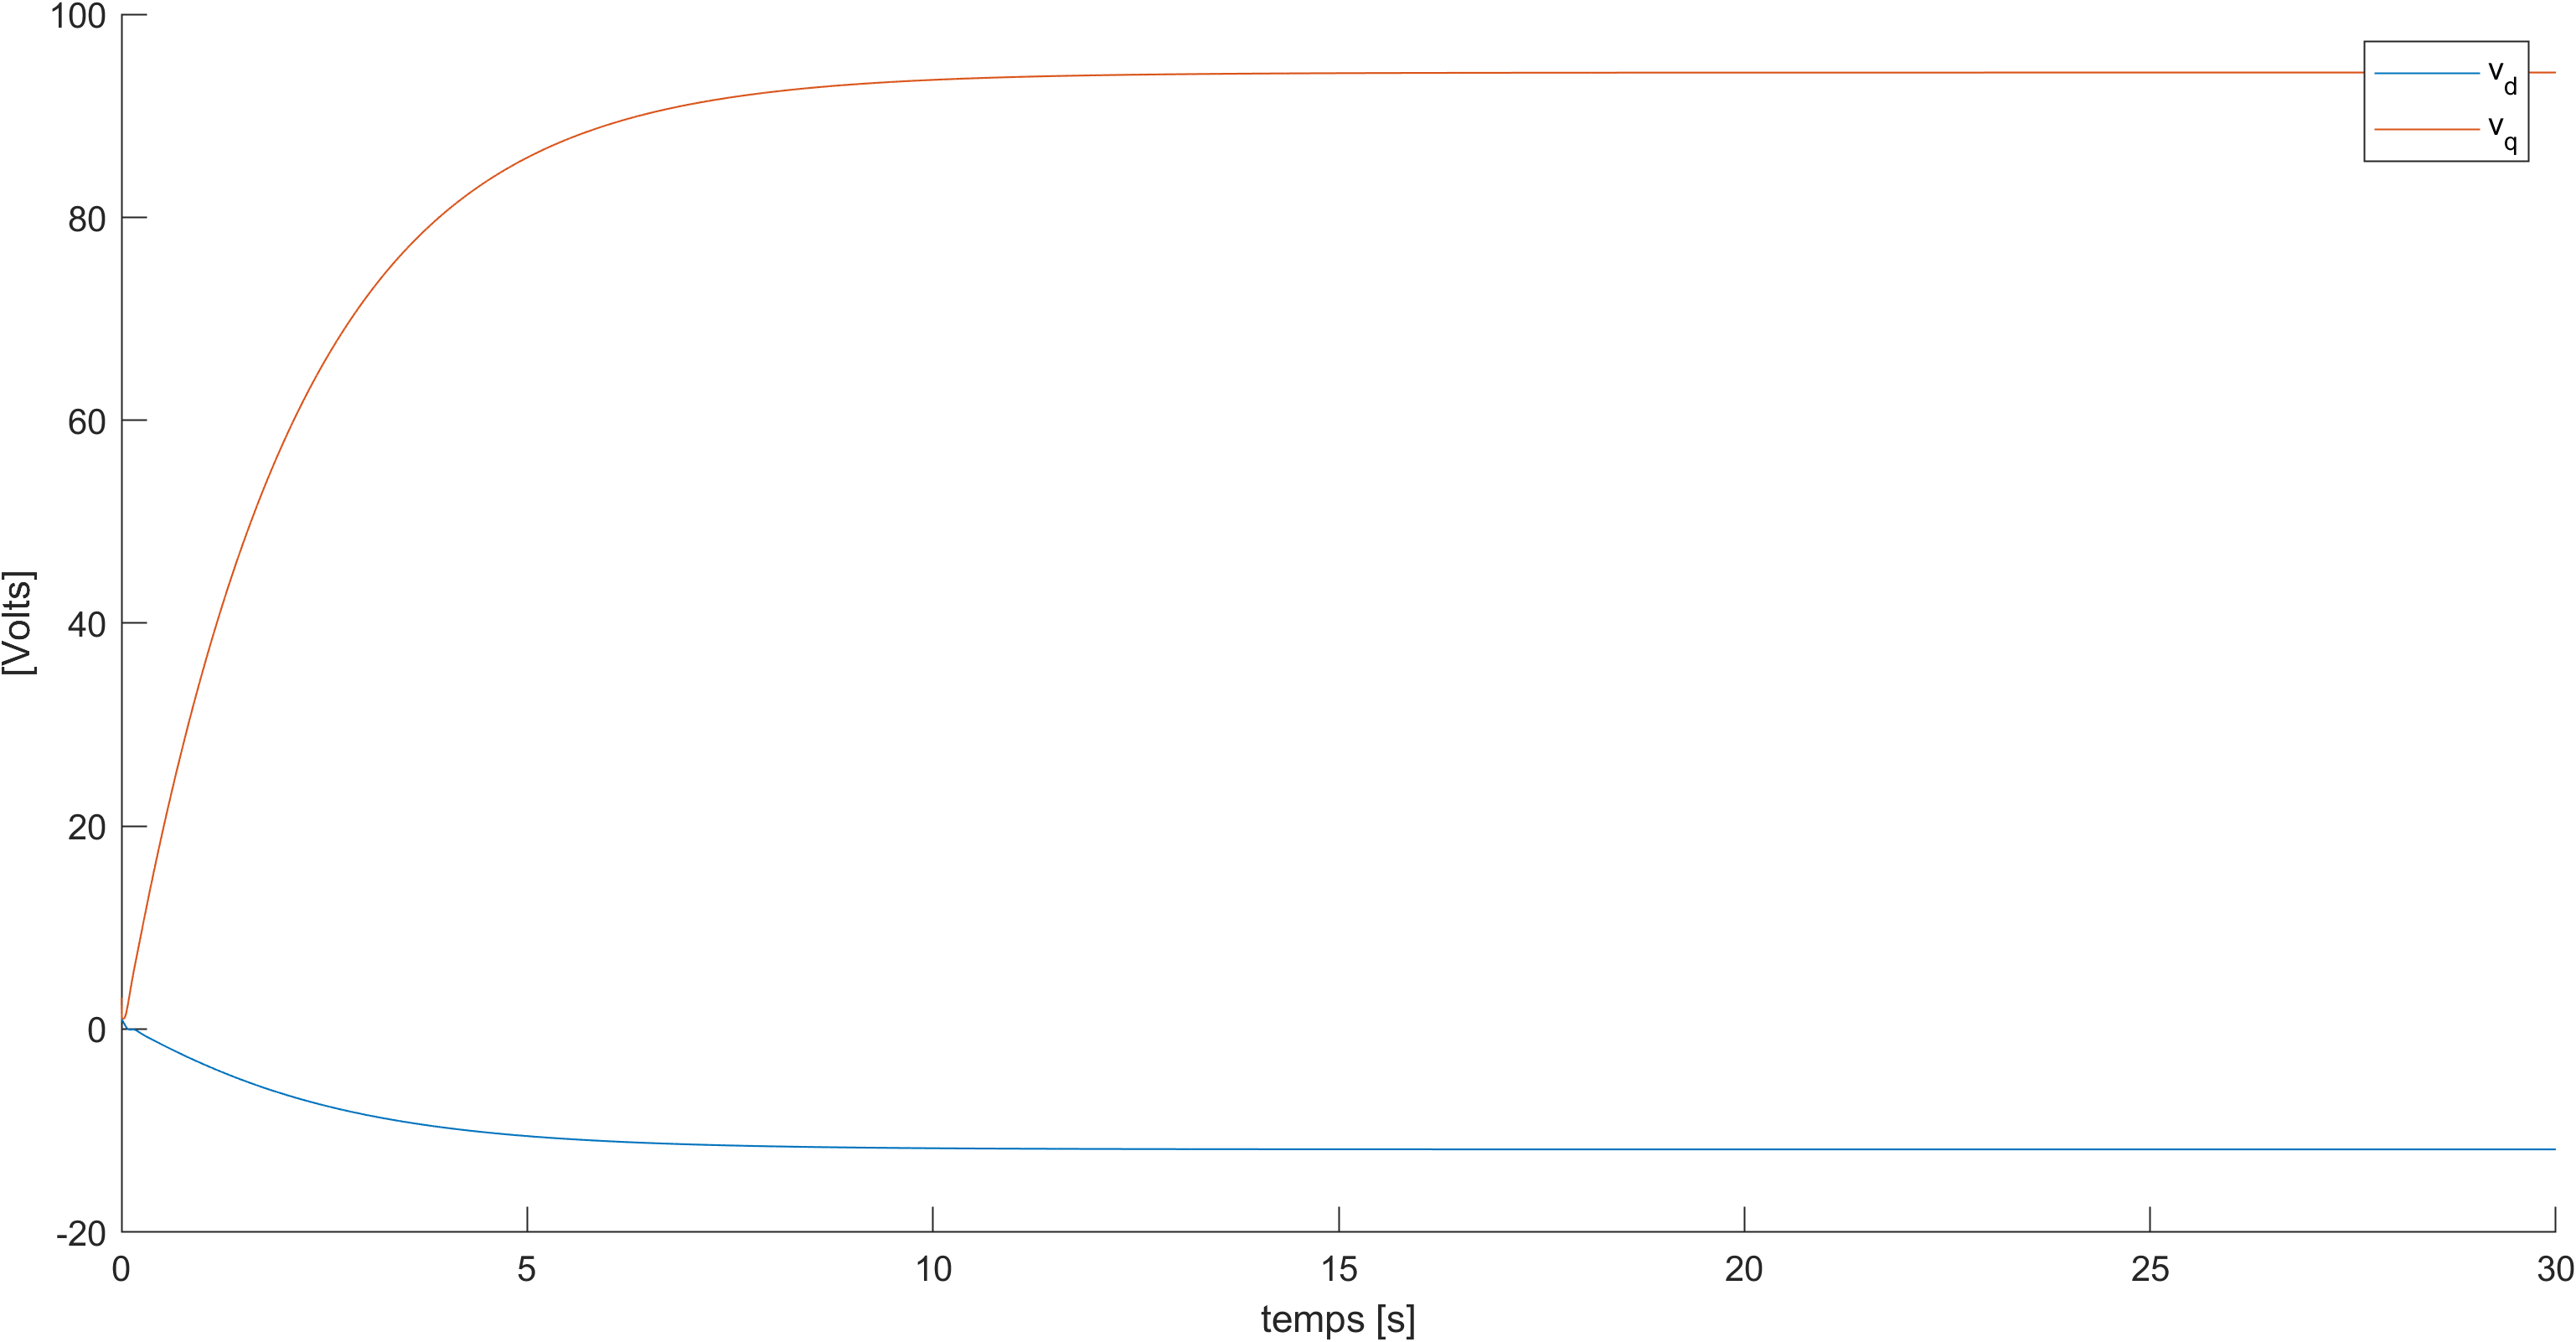
\includegraphics[width=0.8\textwidth]{simusMATLAB/MAS/Vs_dq.png} 
    \caption{Tensions dans le repère dq du stator de la MAS mesurées au cous du temps.}
    \label{img-simuMatlab-Vs_dq}
\end{figure}


\begin{figure}[!h]
    \centering
    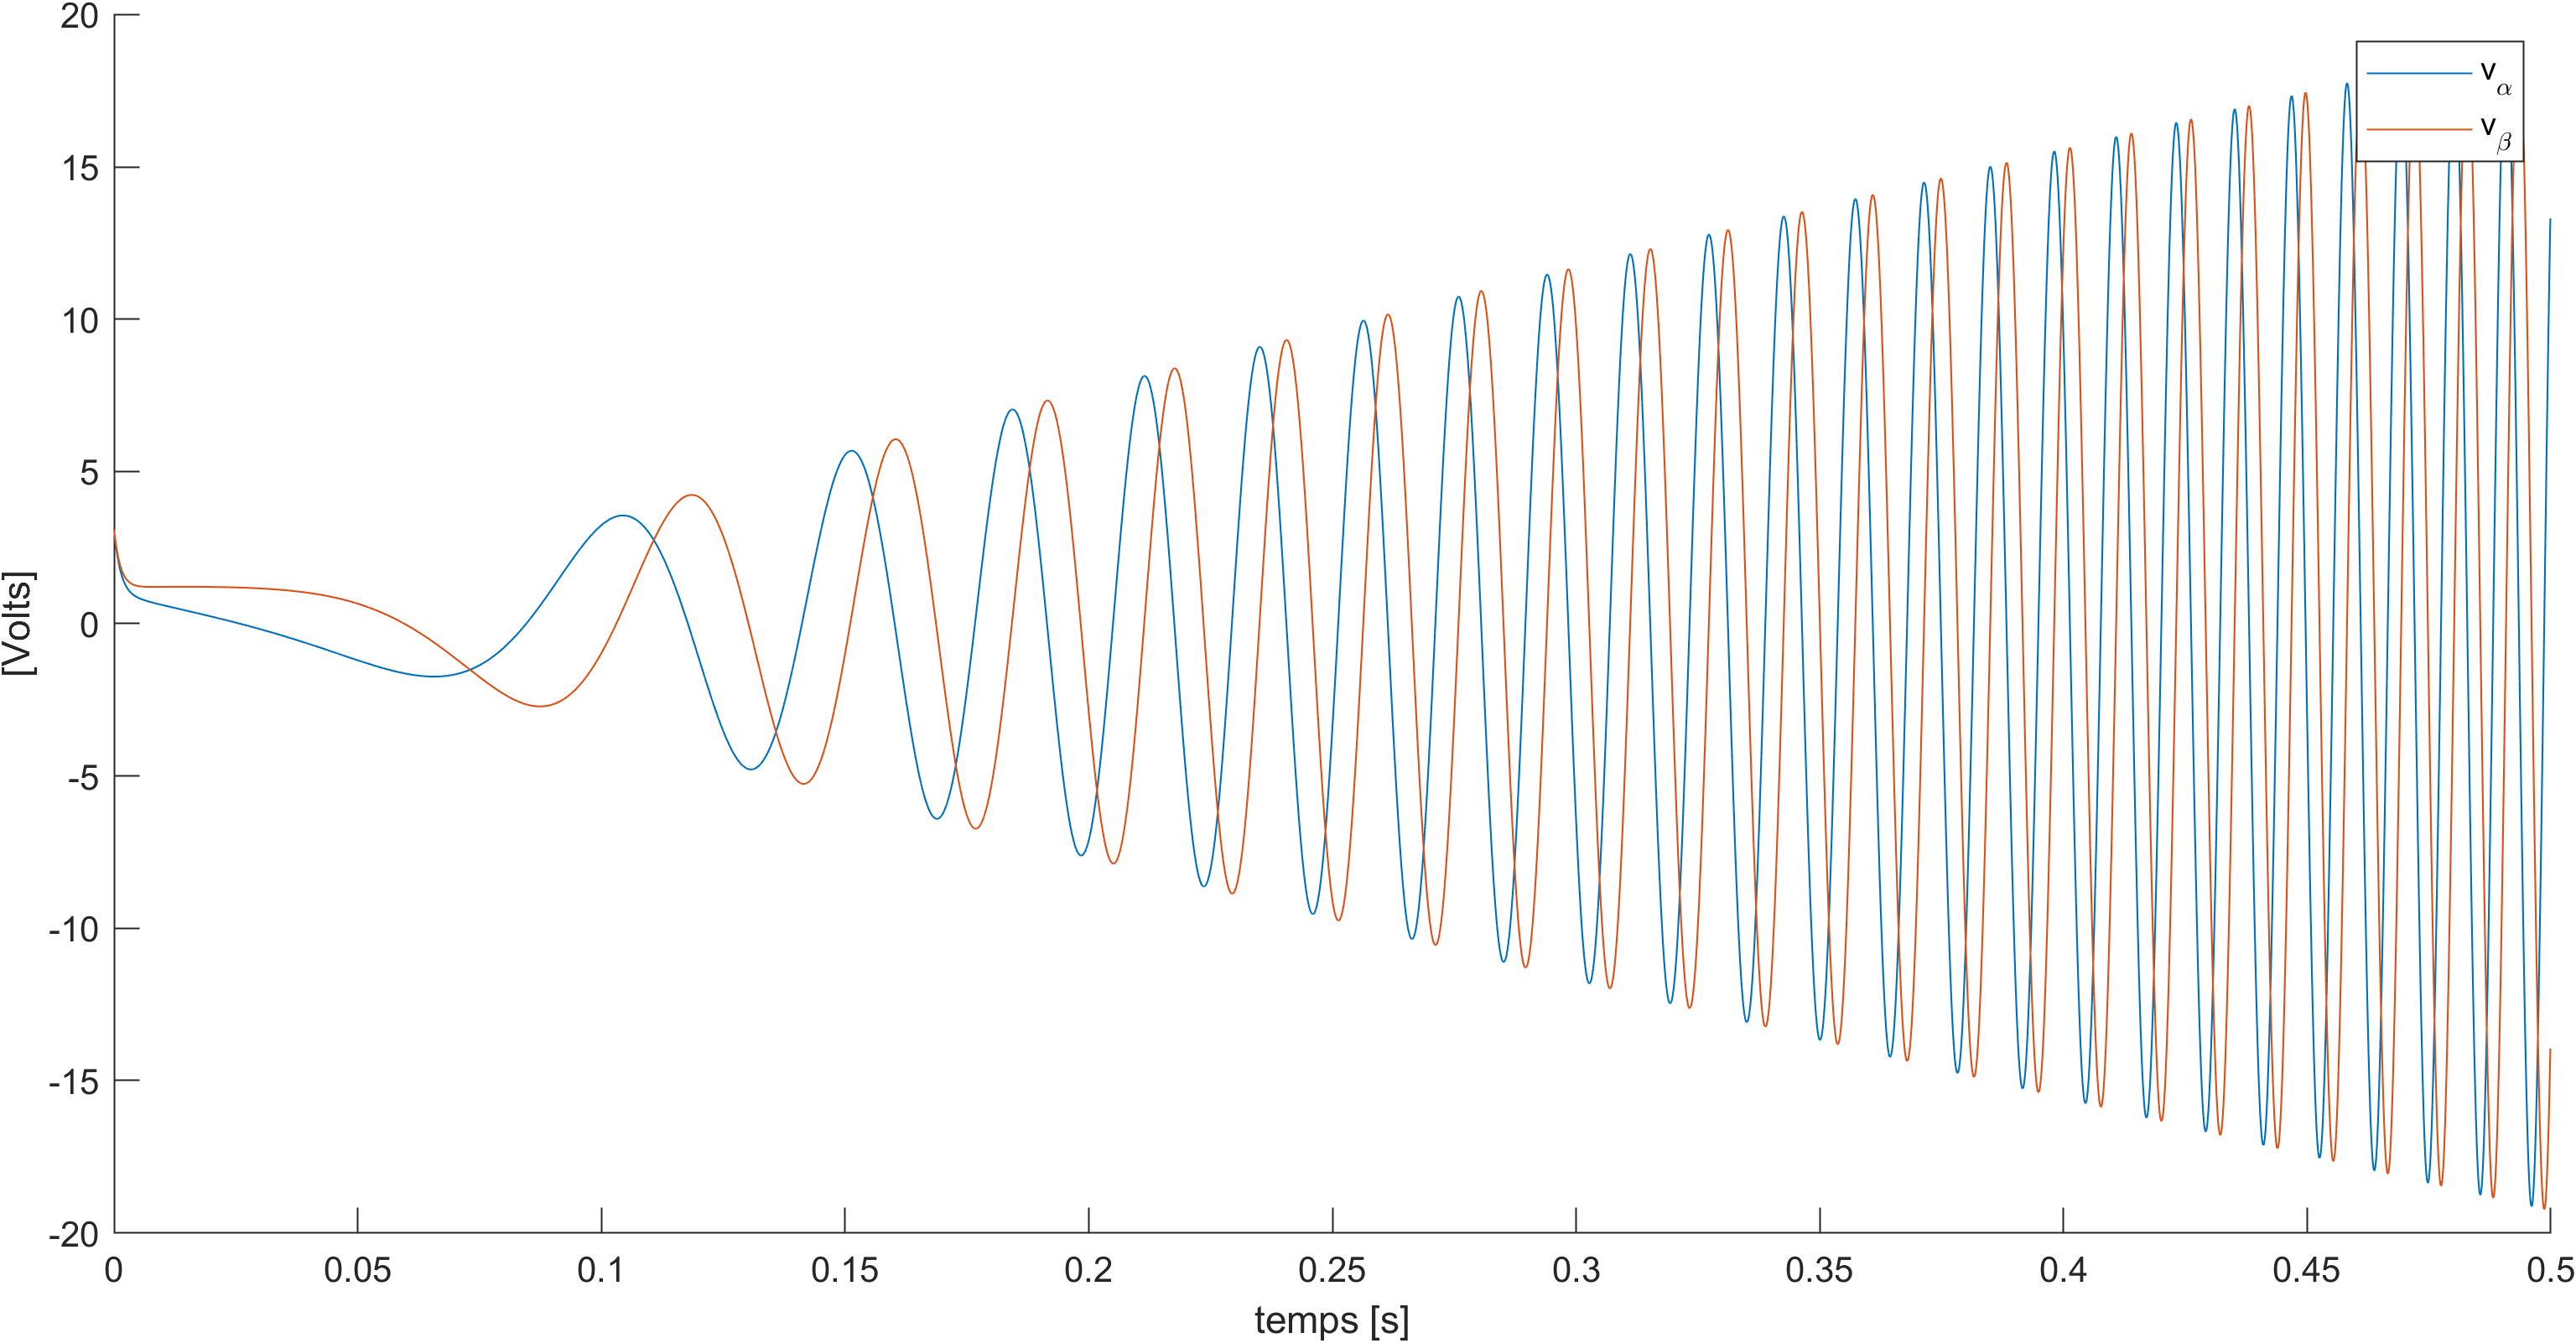
\includegraphics[width=0.8\textwidth]{simusMATLAB/MAS/Vs_alphabeta.png} 
    \caption{Tensions dans le repère $\alpha\beta$ du stator de la MAS mesurées au cous du temps.}
    \label{img-simuMatlab-Vs_alphabeta}
\end{figure}

Pour approfondir la compréhension de la variation angulaire au fil du temps, une analyse de \(\theta_s\) et \(\theta_r\) révèle une augmentation progressive de \(\theta_s\) alors que \(\theta_r\) reste inchangé, reflétant l'absence d'alimentation électrique au rotor. Cette dynamique est clairement exposée, soulignant l'effet de l'alimentation statorique sur la variation angulaire sur la Figure \ref{img-simuMatlab-thetas}.


\begin{figure}[!h]
    \centering
    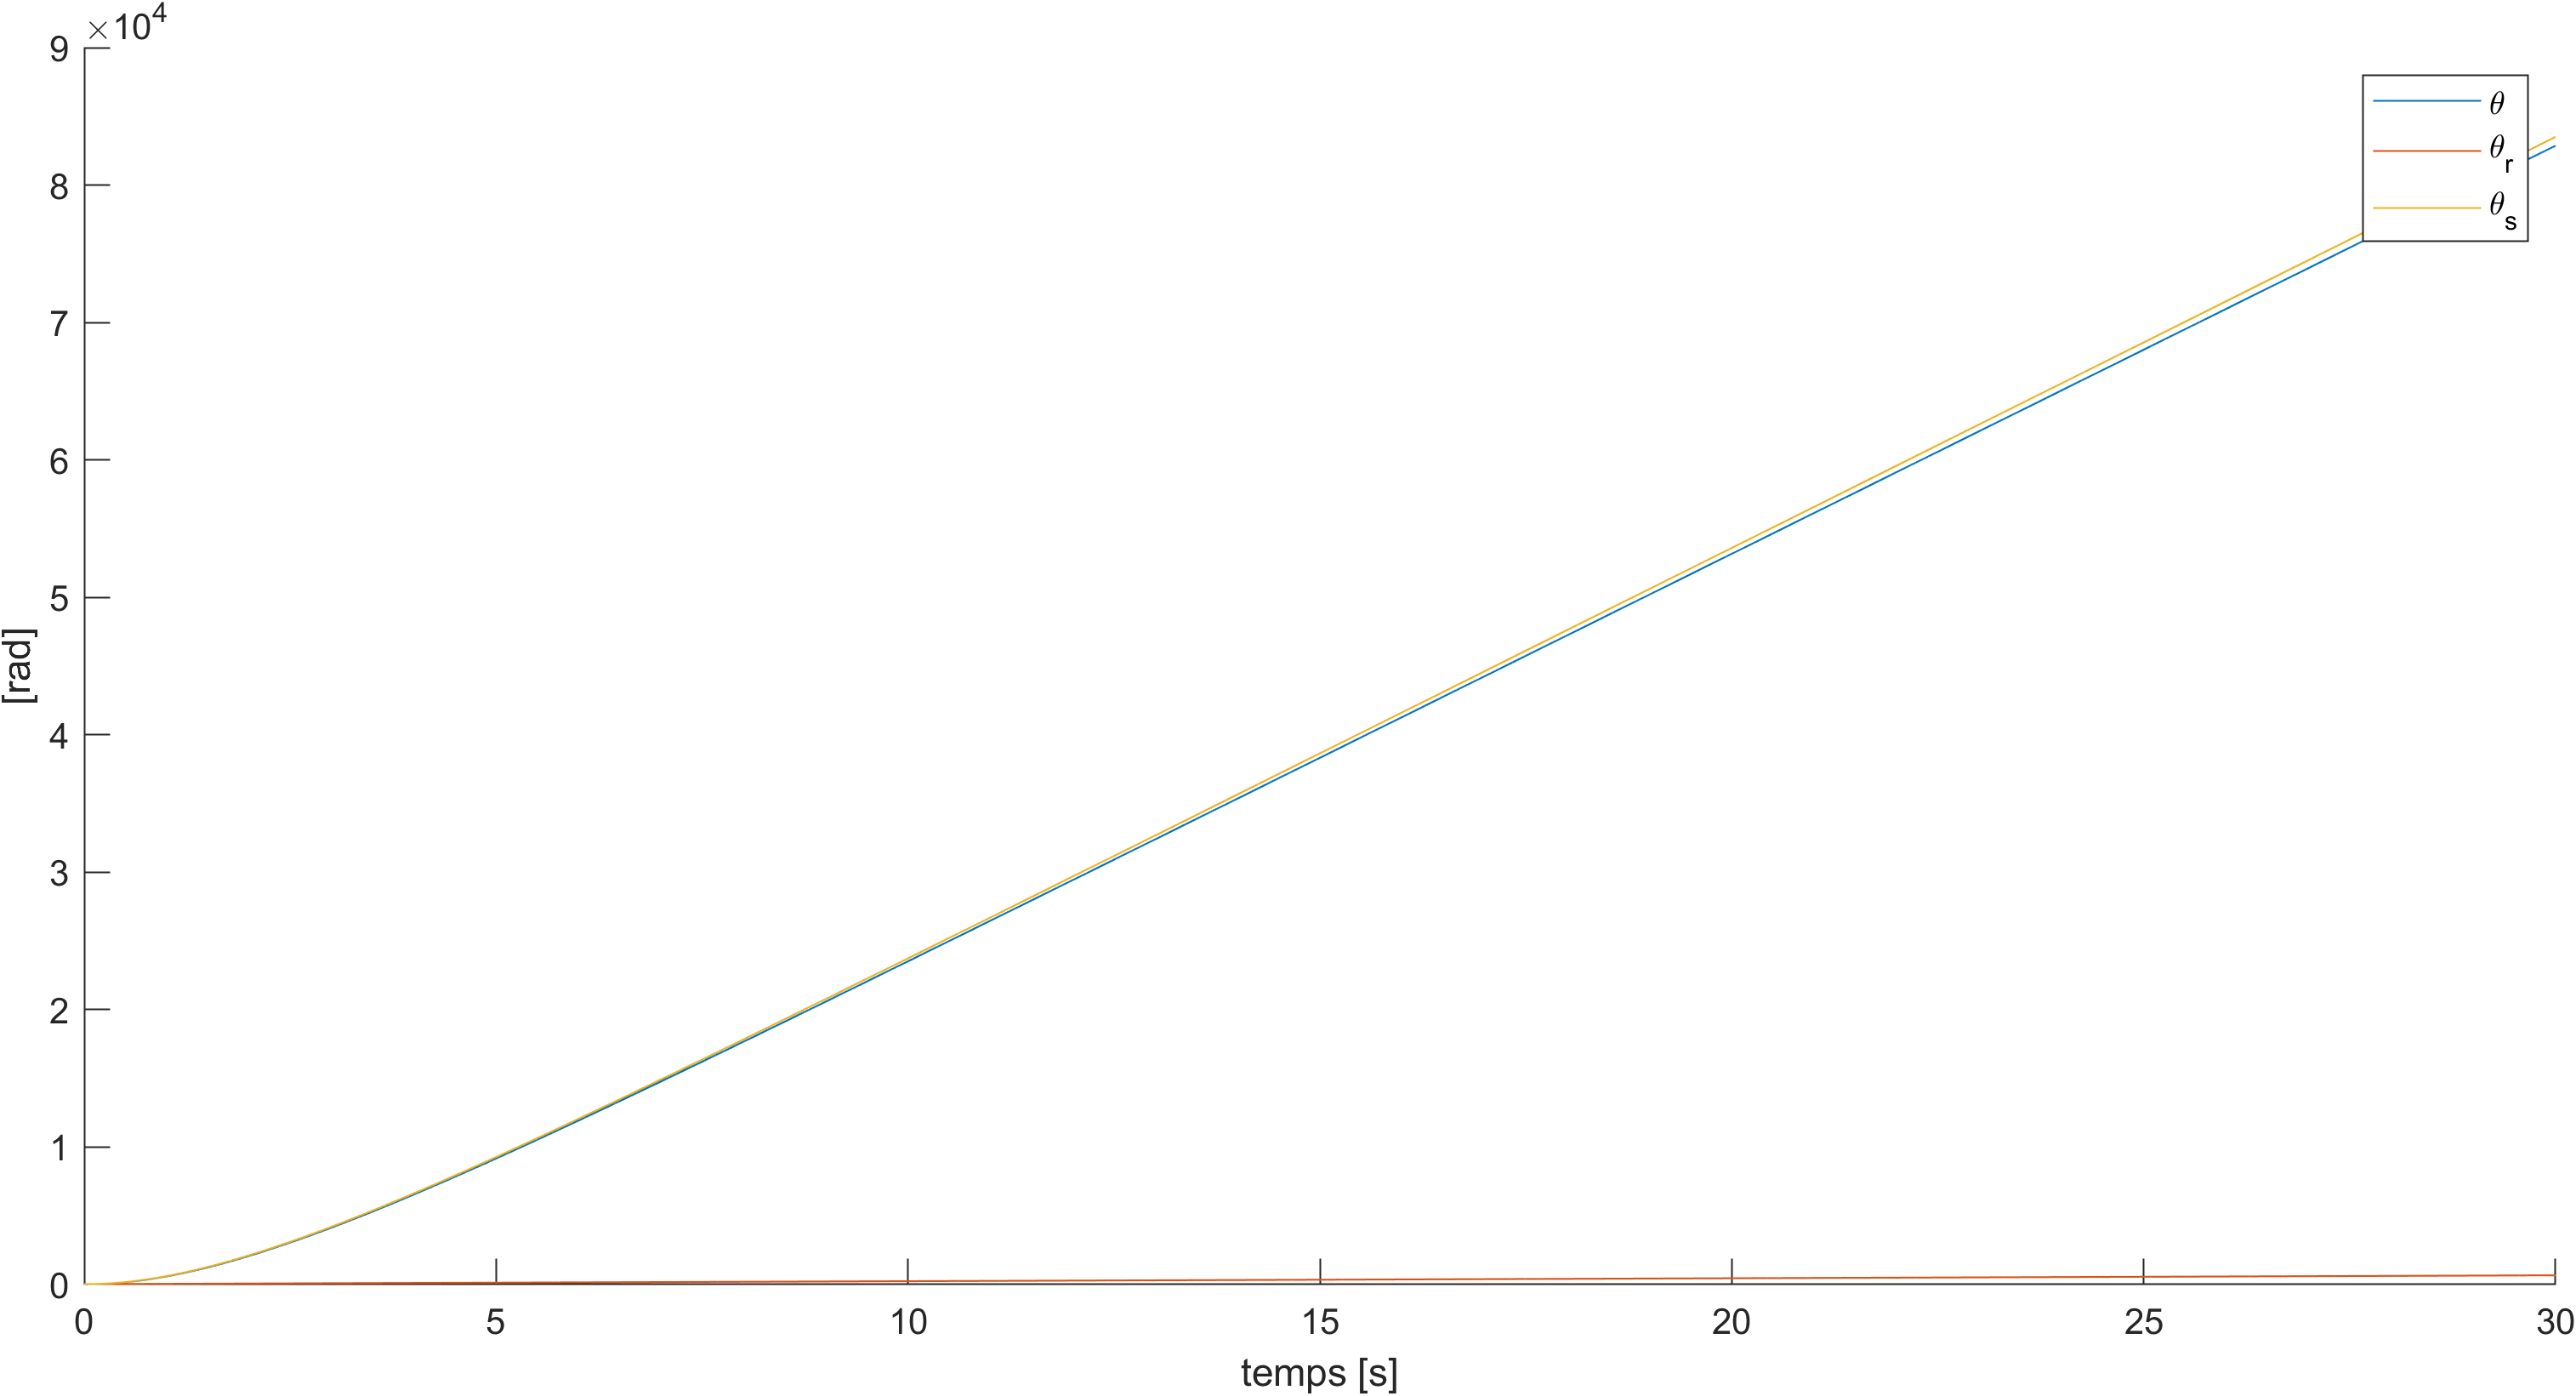
\includegraphics[width=0.8\textwidth]{simusMATLAB/MAS/thetas.png} 
    \caption{Angles de phase des grandeurs de la MAS mesurée au cous du temps.}
    \label{img-simuMatlab-thetas}
\end{figure}


L'angle \(\theta\), observé dans la Figure \ref{img-simuMatlab-thetas}, permet de visualiser le mouvement des grandeurs rotoriques dans le temps. En appliquant cet angle variable, c'est possible de suivre la rotation des composantes du rotor, illustrant ainsi leur évolution dynamique au fil du temps comme exposée dans les Figures \ref{img-simuMatlab-ir_abc} et \ref{img-simuMatlab-ir_dq}.


\begin{figure}[!h]
    \centering
    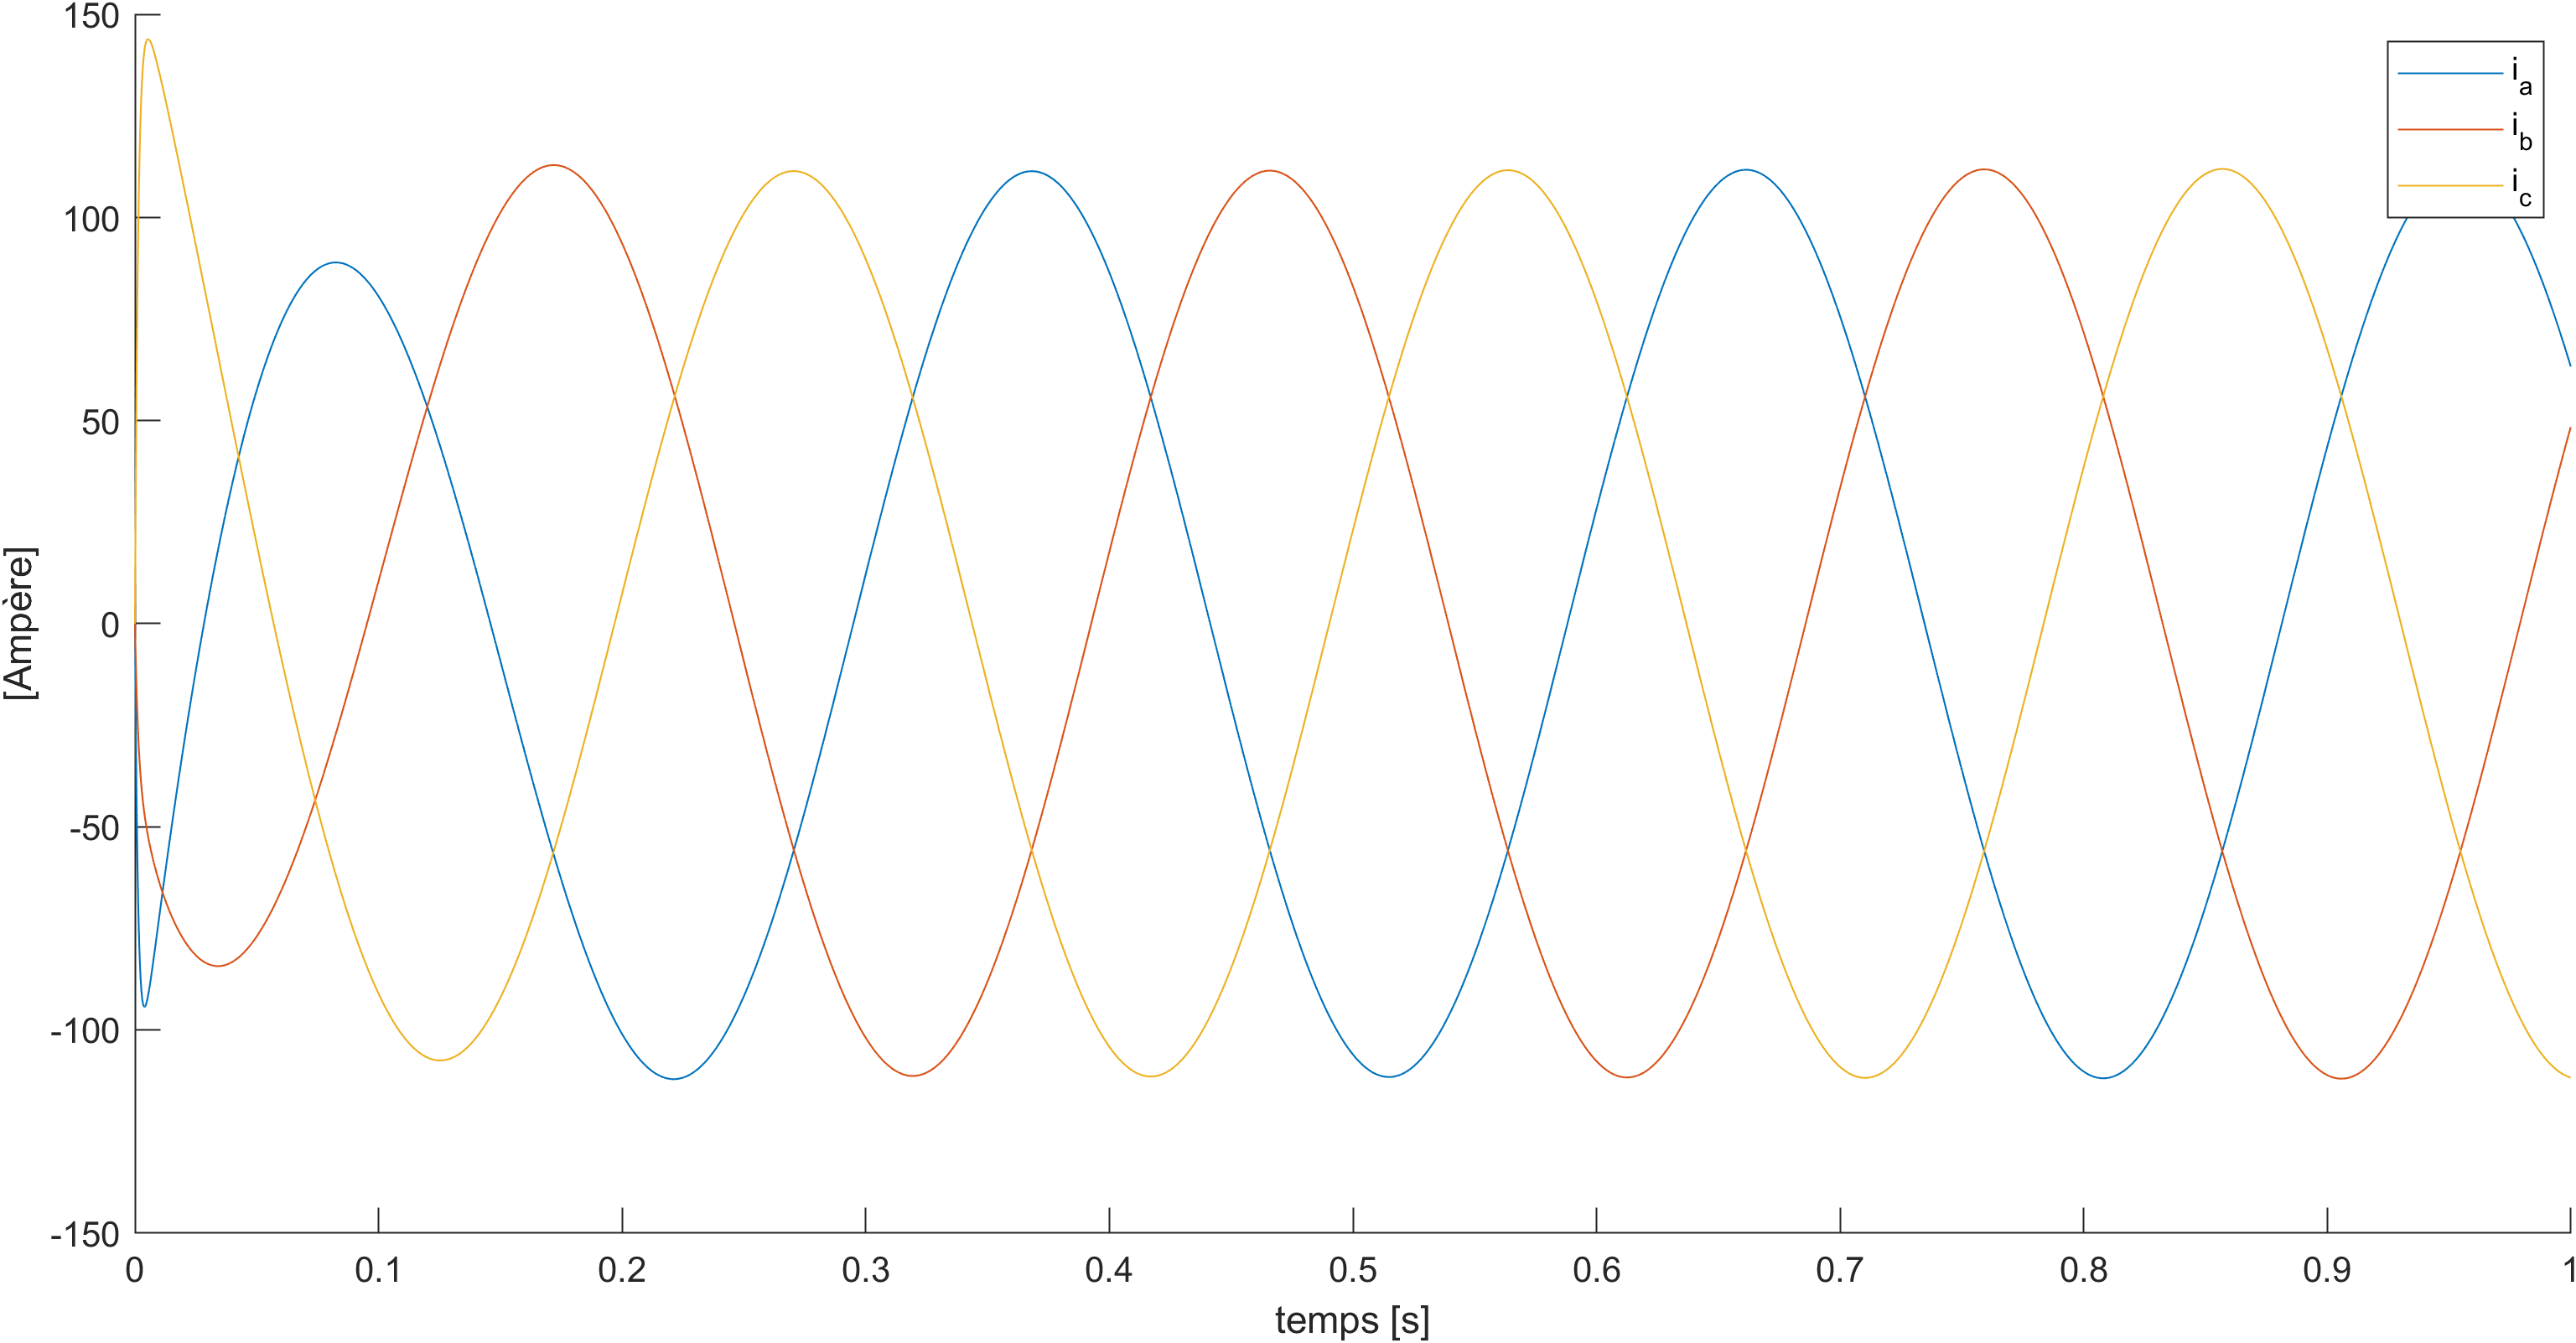
\includegraphics[width=0.8\textwidth]{simusMATLAB/MAS/ir_abc.png} 
    \caption{Courants triphasées du rotor de la MAS mesurées au cours du temps.}
    \label{img-simuMatlab-ir_abc}
\end{figure}

\begin{figure}[!h]
    \centering
    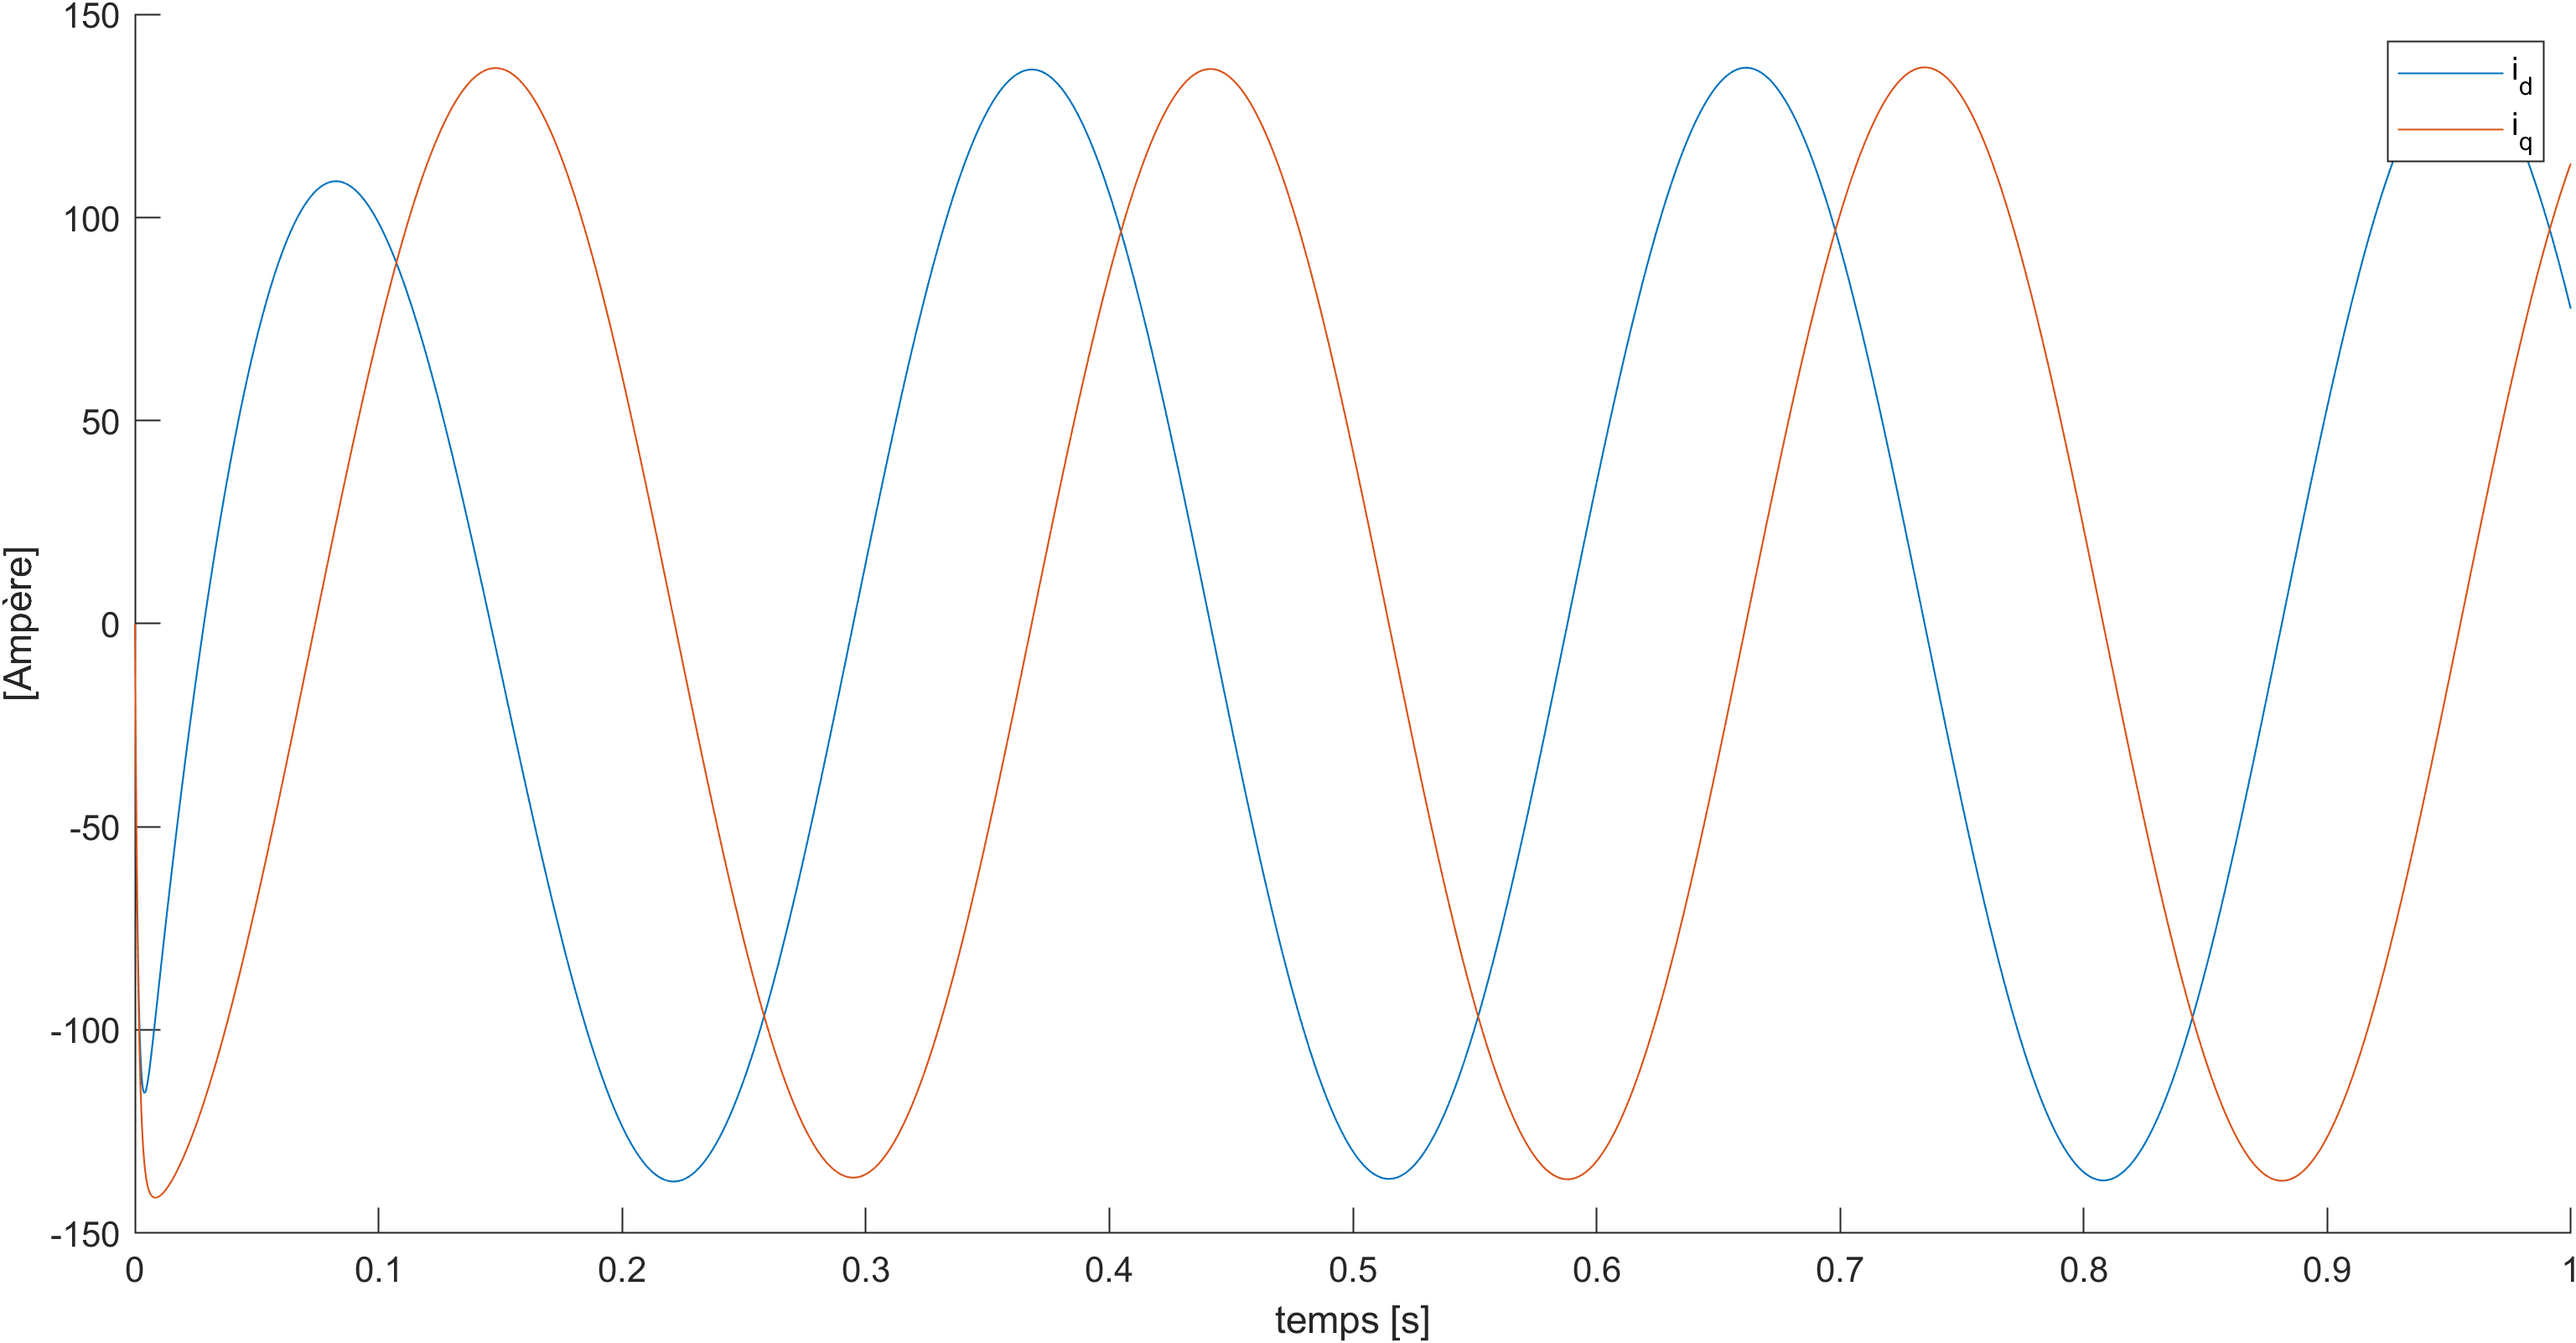
\includegraphics[width=0.8\textwidth]{simusMATLAB/MAS/ir_dq.png} 
    \caption{Courants dans le repère dq du rotor de la MAS au cous du temps.}
    \label{img-simuMatlab-ir_dq}
\end{figure}


Au-delà des mesures de tension et de courant, l'analyse de la courbe de couple de la machine (Figure \ref{img-simuMatlab-Ce}) offre un aperçu de la force de rotation disponible, depuis le démarrage jusqu'à la stabilisation de la vitesse. Cette courbe est indispensable pour évaluer la capacité de la machine à monter en vitesse rapidement et son comportement face aux démarrages fréquents, offrant ainsi une compréhension de ses performances et de sa réactivité.


\begin{figure}[!h]
    \centering
    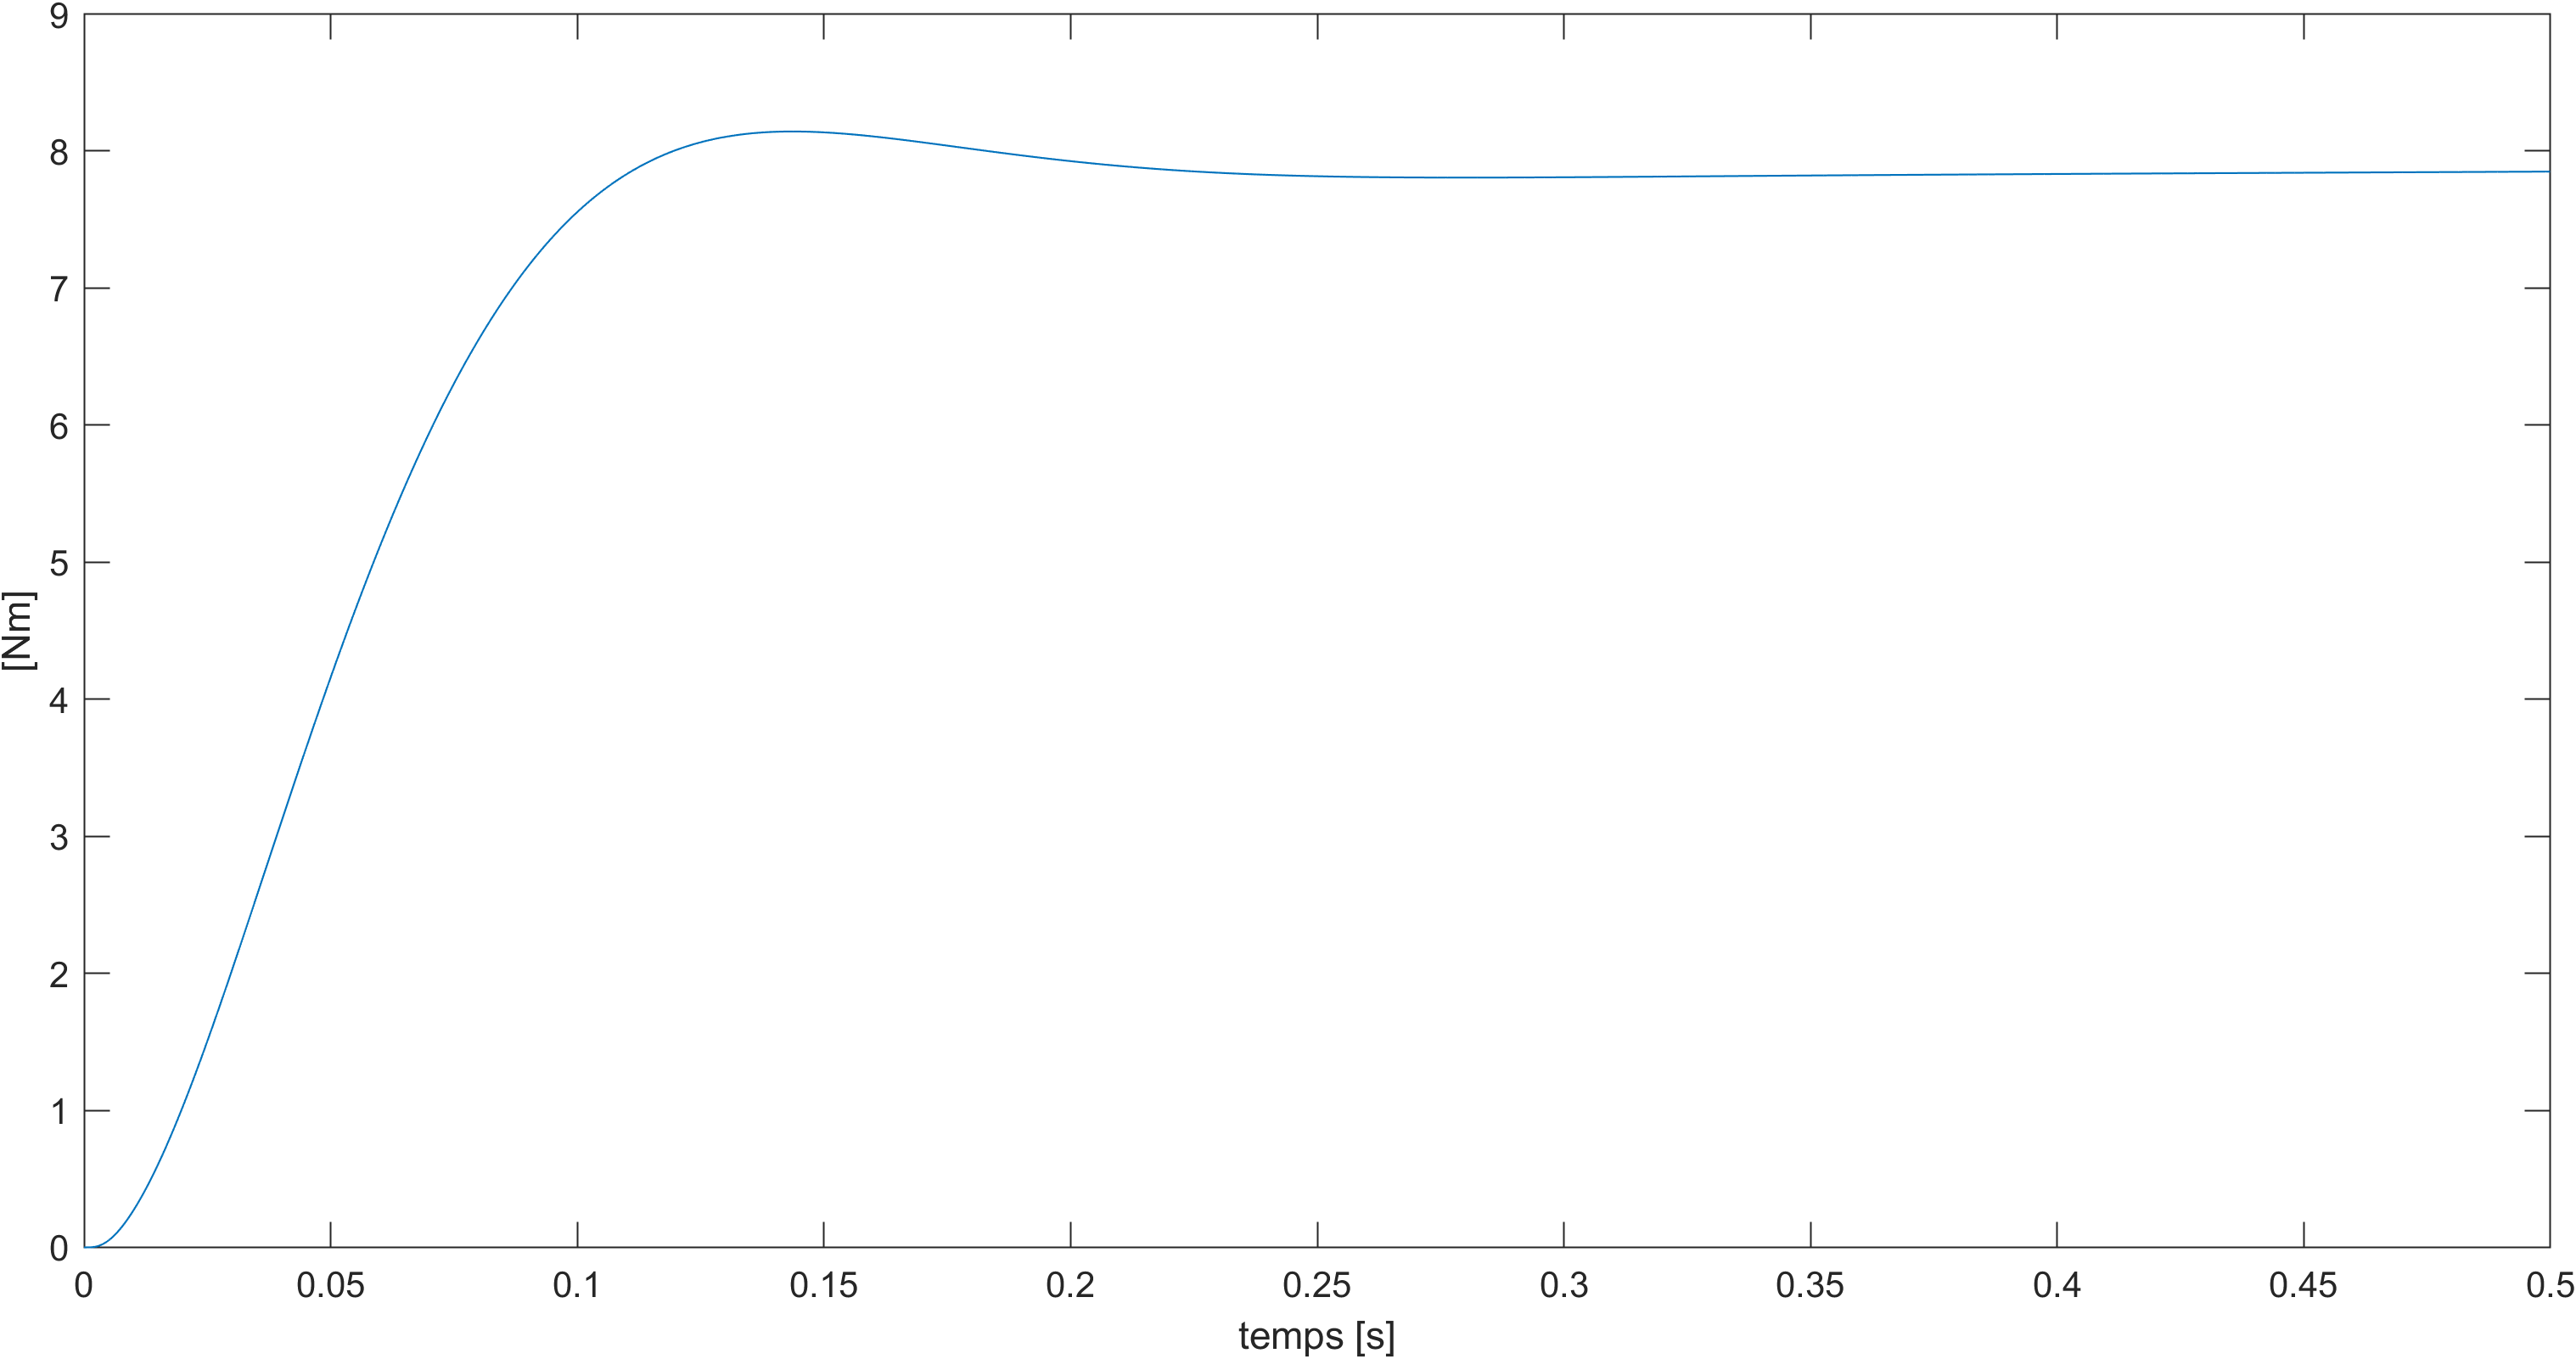
\includegraphics[width=0.8\textwidth]{simusMATLAB/MAS/Ce.png} 
    \caption{Couple de la MAS mesurée au cous du temps.}
    \label{img-simuMatlab-Ce}
\end{figure}

D'autres grandeurs qui ont été mesurées, sont la puissance, flux et torque de la machine, dans les Figures \ref{img-simuMatlab-P}, \ref{img-simuMatlab-phi_r} et \ref{img-simuMatlab-torque} respectivement. C'est possible de voir comme le flux induit dans le rotor de la machine augmente dans un intervalle très court de temps, dans la Figure \ref{img-simuMatlab-phi_r}.


\begin{figure}[!h]
    \centering
    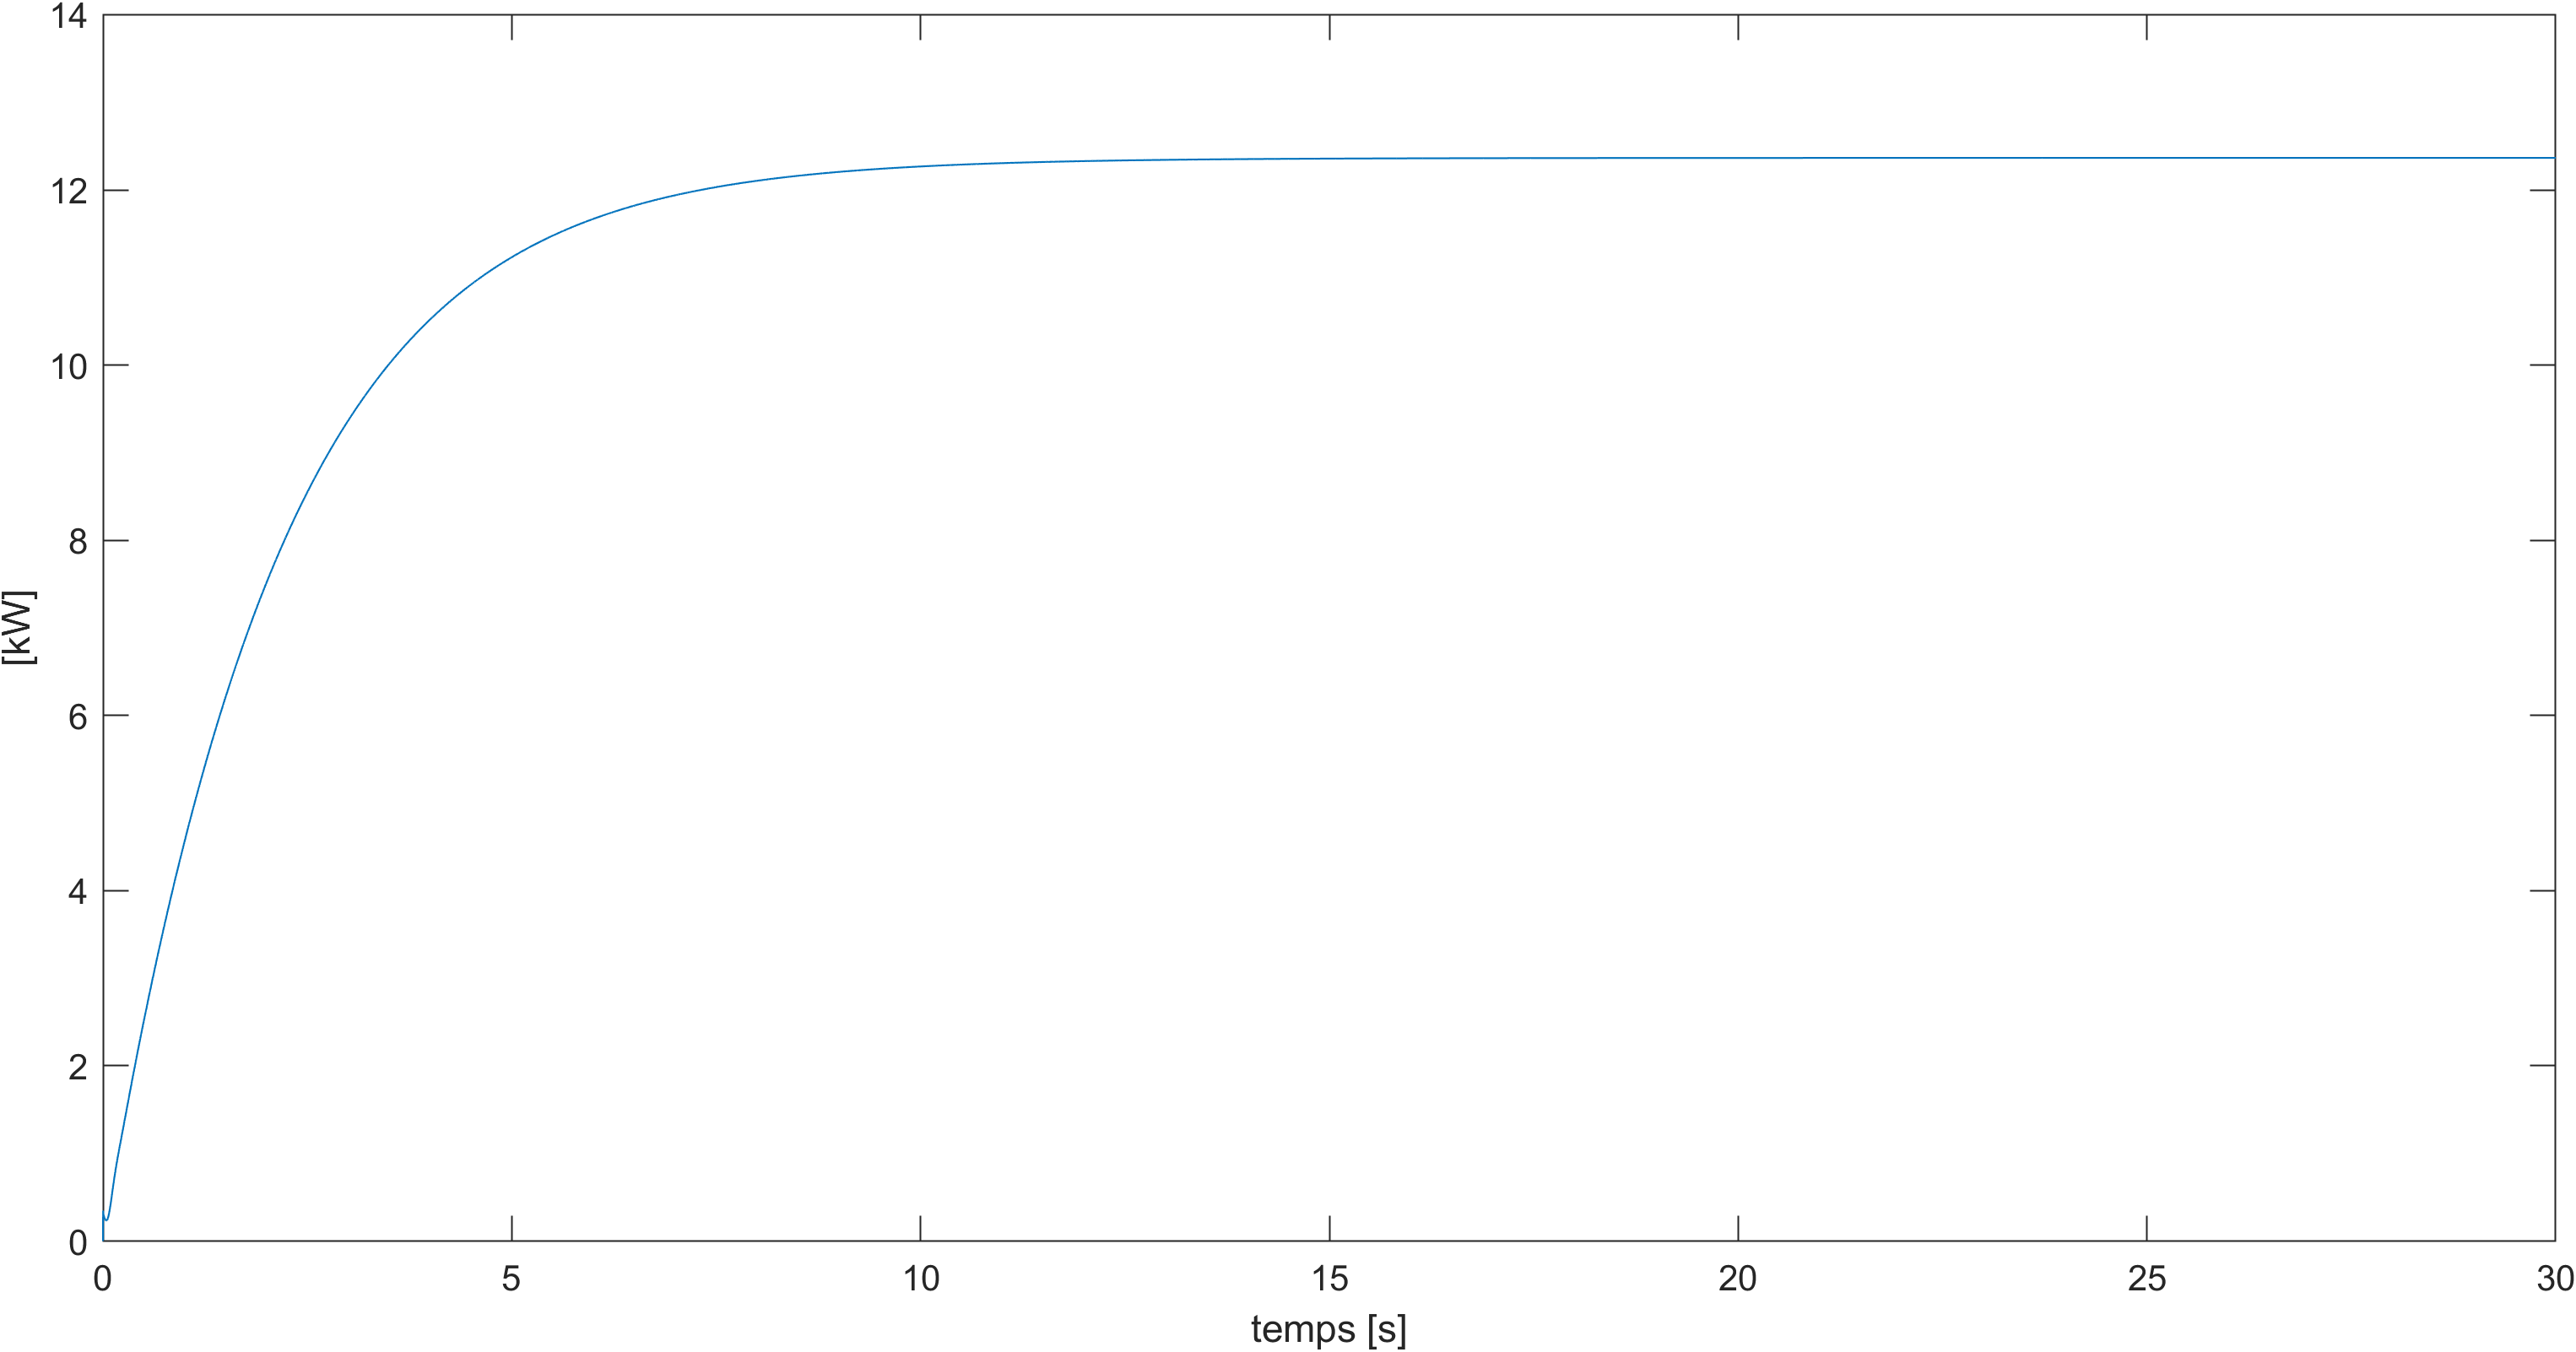
\includegraphics[width=0.8\textwidth]{simusMATLAB/MAS/P.png} 
    \caption{Puissance de la MAS mesurée au cous du temps.}
    \label{img-simuMatlab-P}
\end{figure}




\begin{figure}[!h]
    \centering
    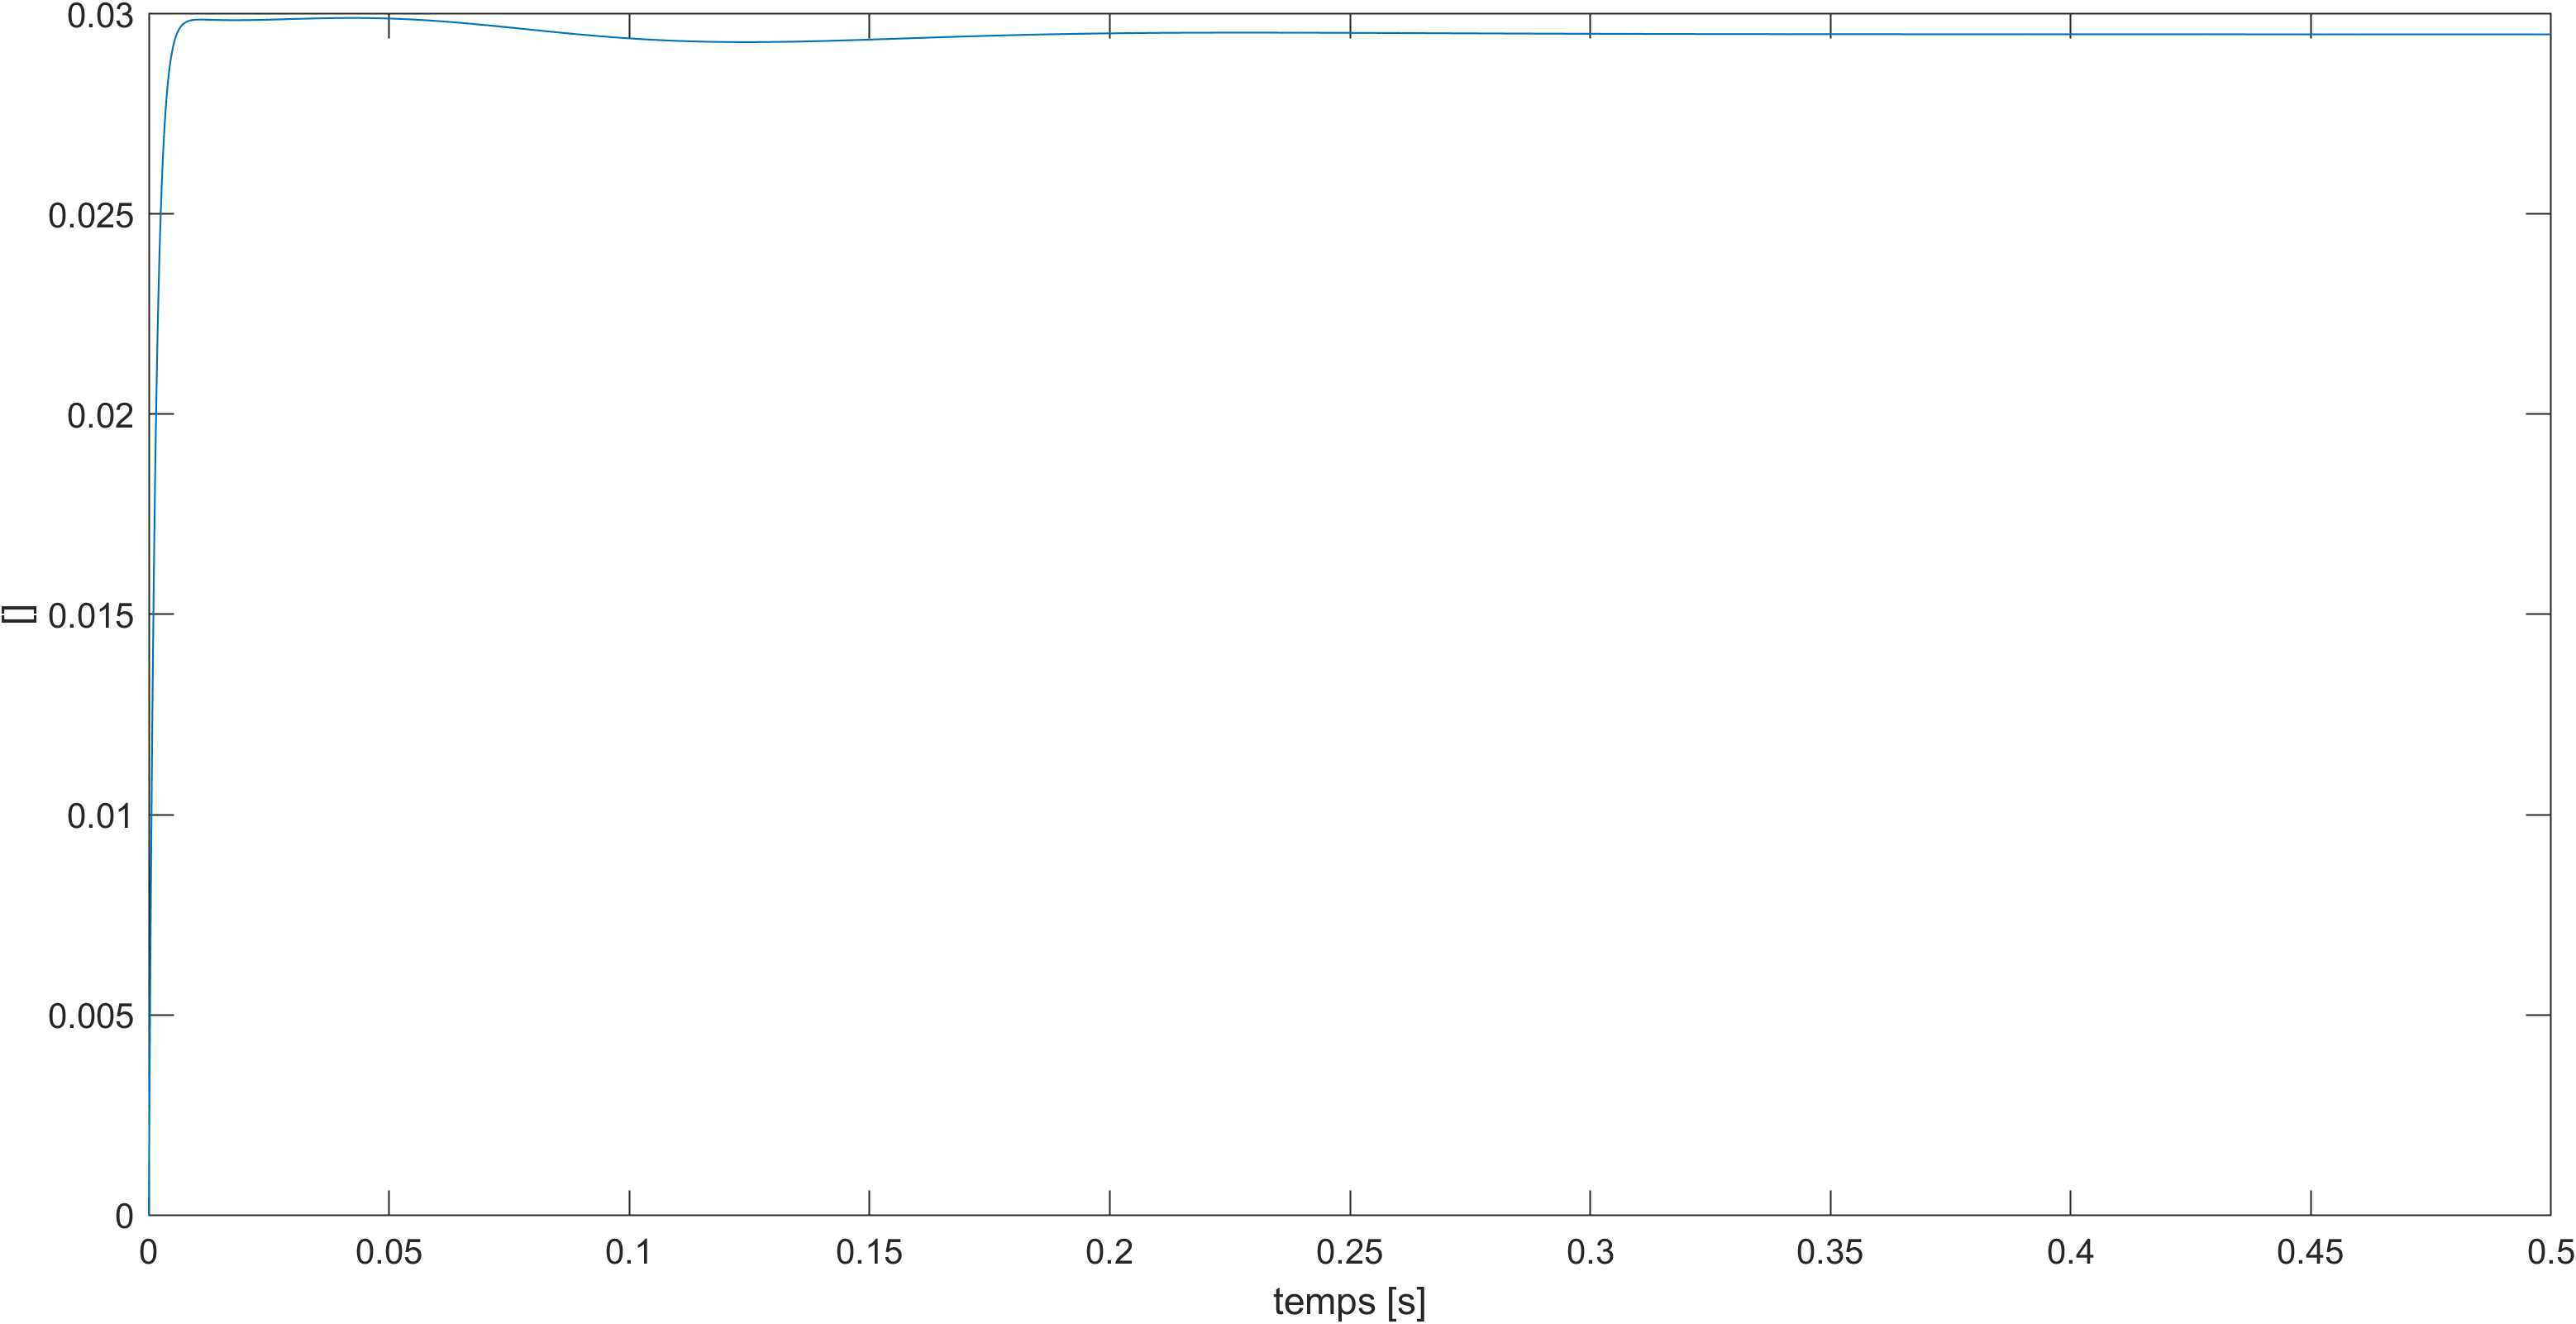
\includegraphics[width=0.8\textwidth]{simusMATLAB/MAS/phi_r.png} 
    \caption{Flux dans le rotor de la MAS mesurée au cous du temps.}
    \label{img-simuMatlab-phi_r}
\end{figure}



\begin{figure}[!h]
    \centering
    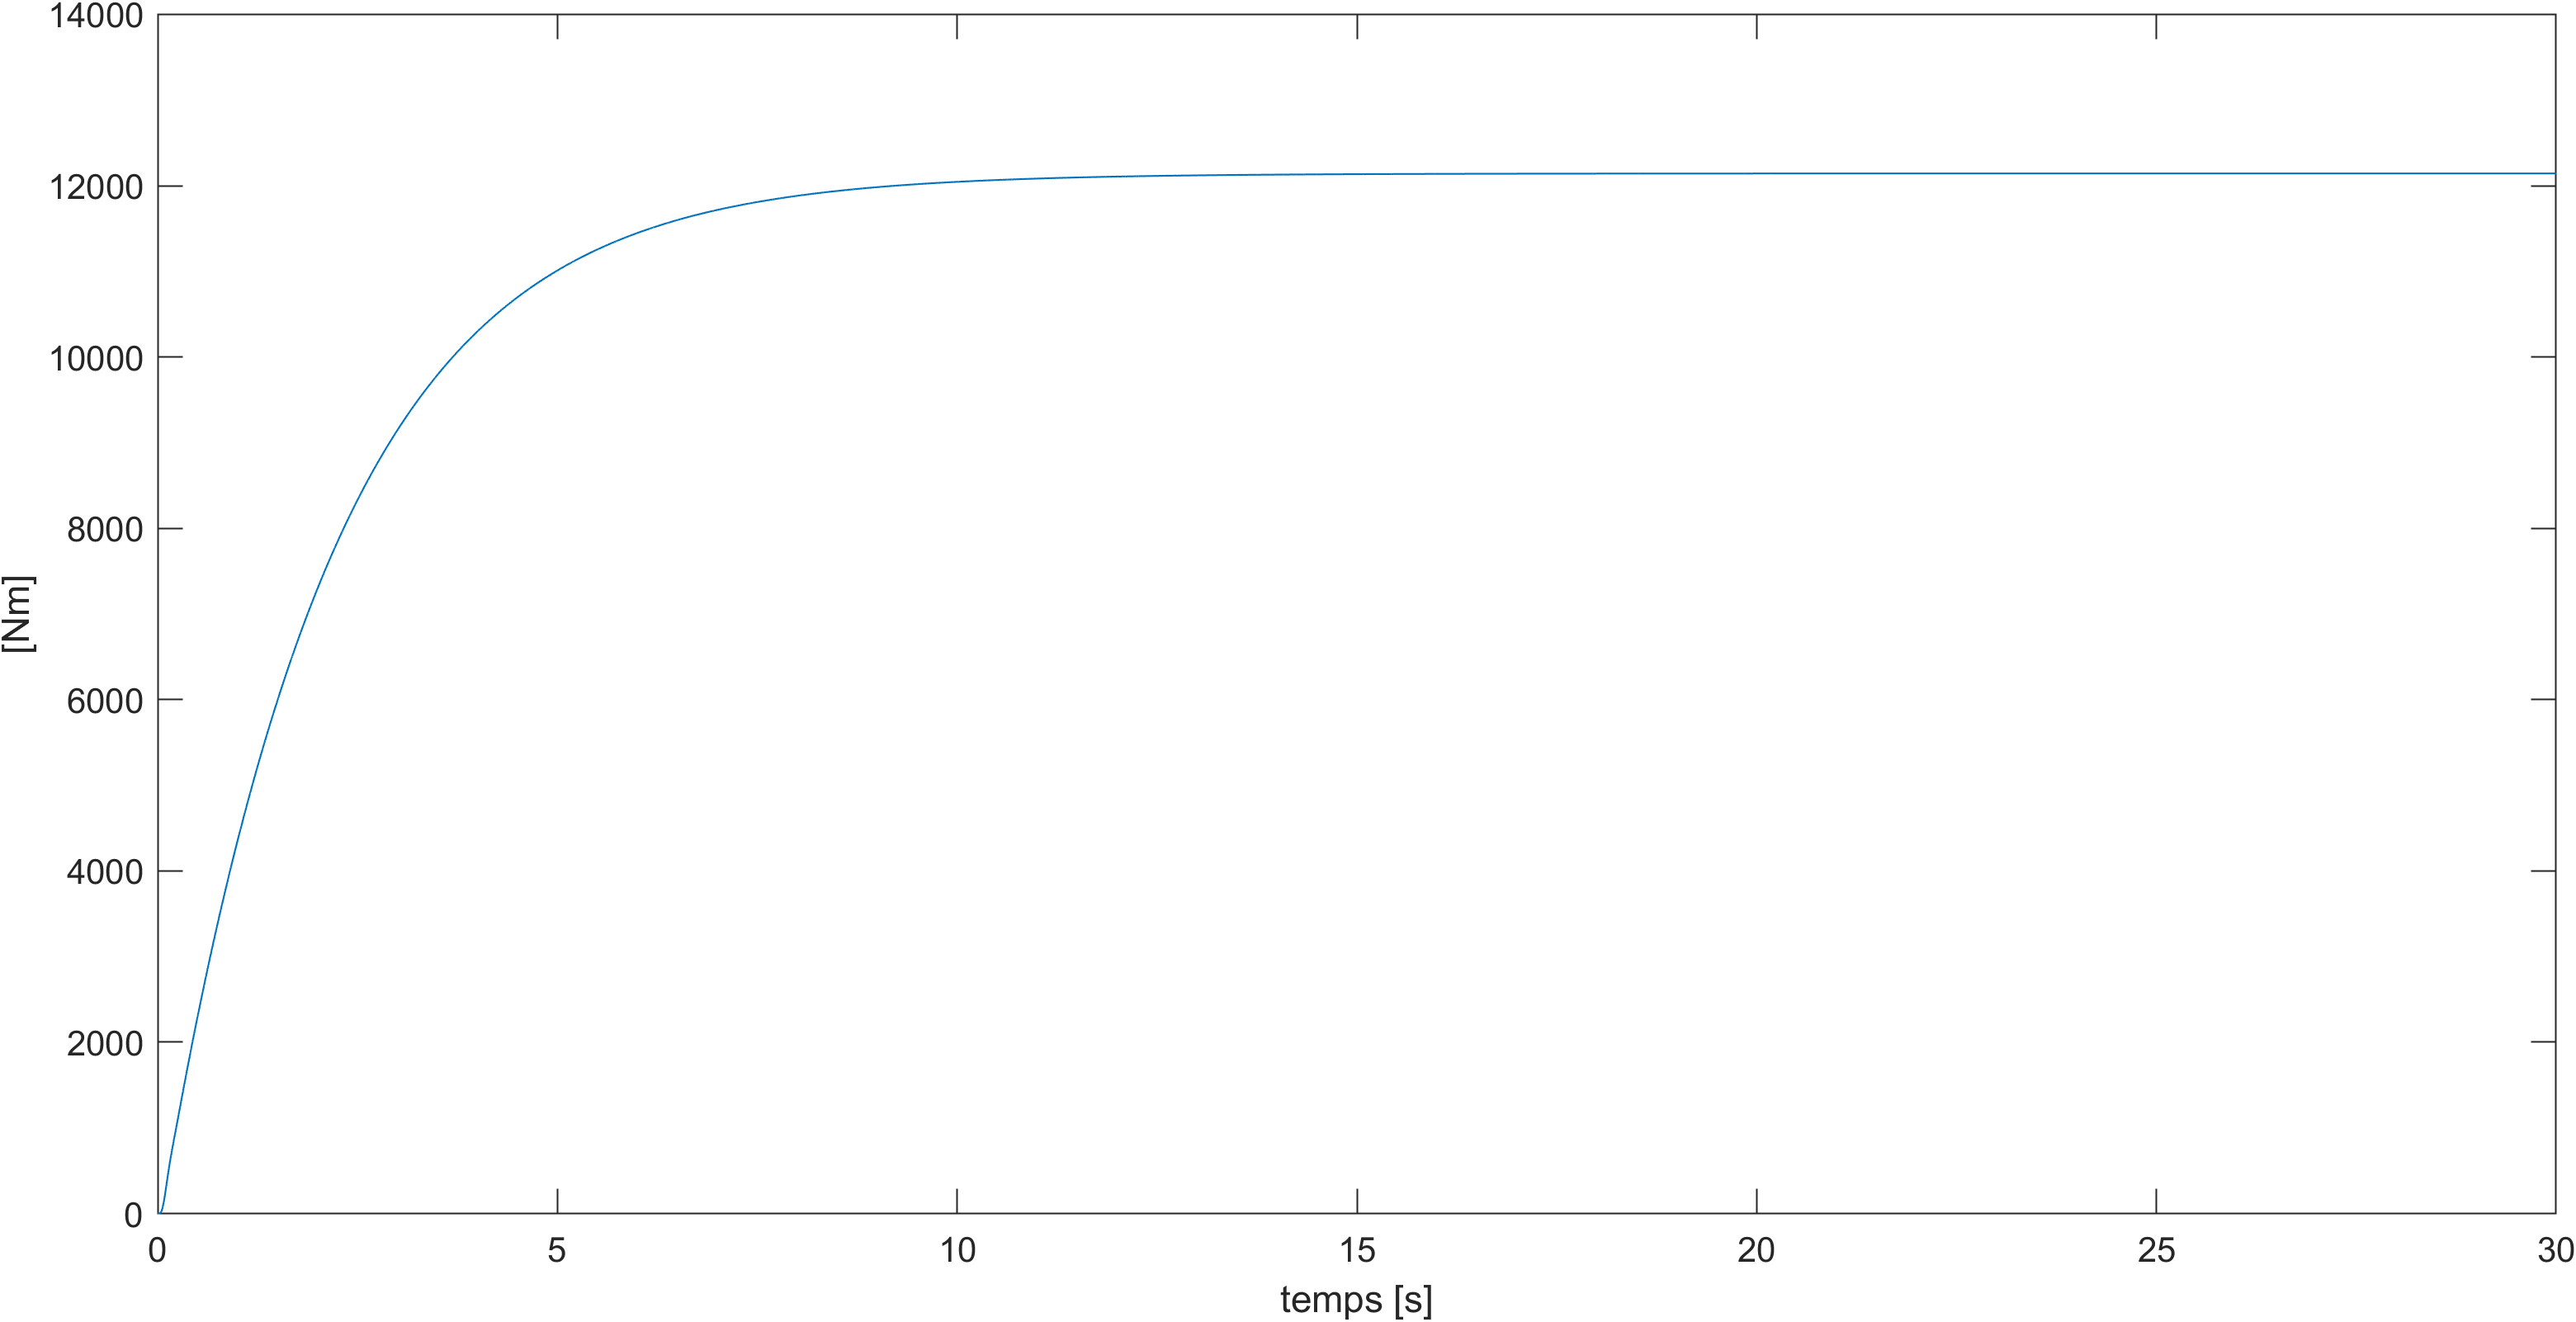
\includegraphics[width=0.8\textwidth]{simusMATLAB/MAS/torque.png} 
    \caption{Torque de la MAS mesurée au cours du temps.}
    \label{img-simuMatlab-torque}
\end{figure}

Afin de vérifier que le système est cohérent dans le régime permanent, deux autres relations du modèle ont été vérifiées, comme le montre le diagramme de la Figure \ref{img-CI_verifier_relations}. Les figures \ref{img-simuMatlab-comparation_wm} et \ref{img-simuMatlab-relation} montrent que le système converge dans le régime permanent. 

\begin{figure}[!h]
    \centering
    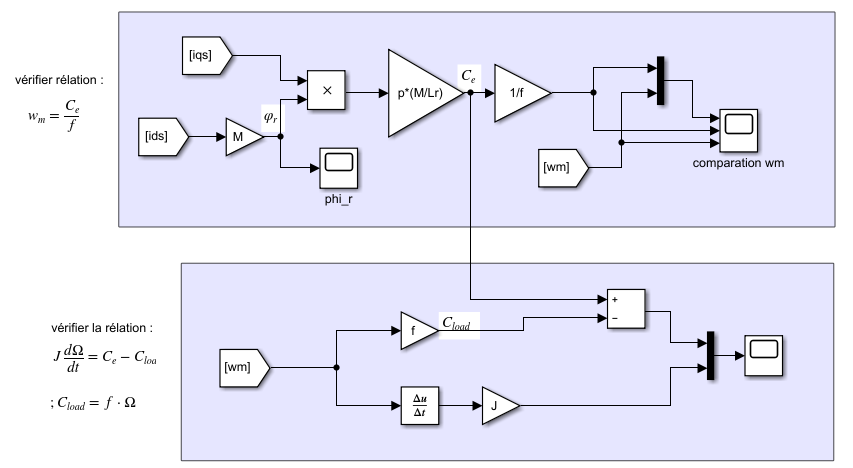
\includegraphics[width=0.9\textwidth]{imgsMATLAB/MAS/CI/CI_verifier_relations.png} 
    \caption{Schémas de validation du modèle de la MAS.}
    \label{img-CI_verifier_relations}
\end{figure}



\begin{figure}[!h]
    \centering
    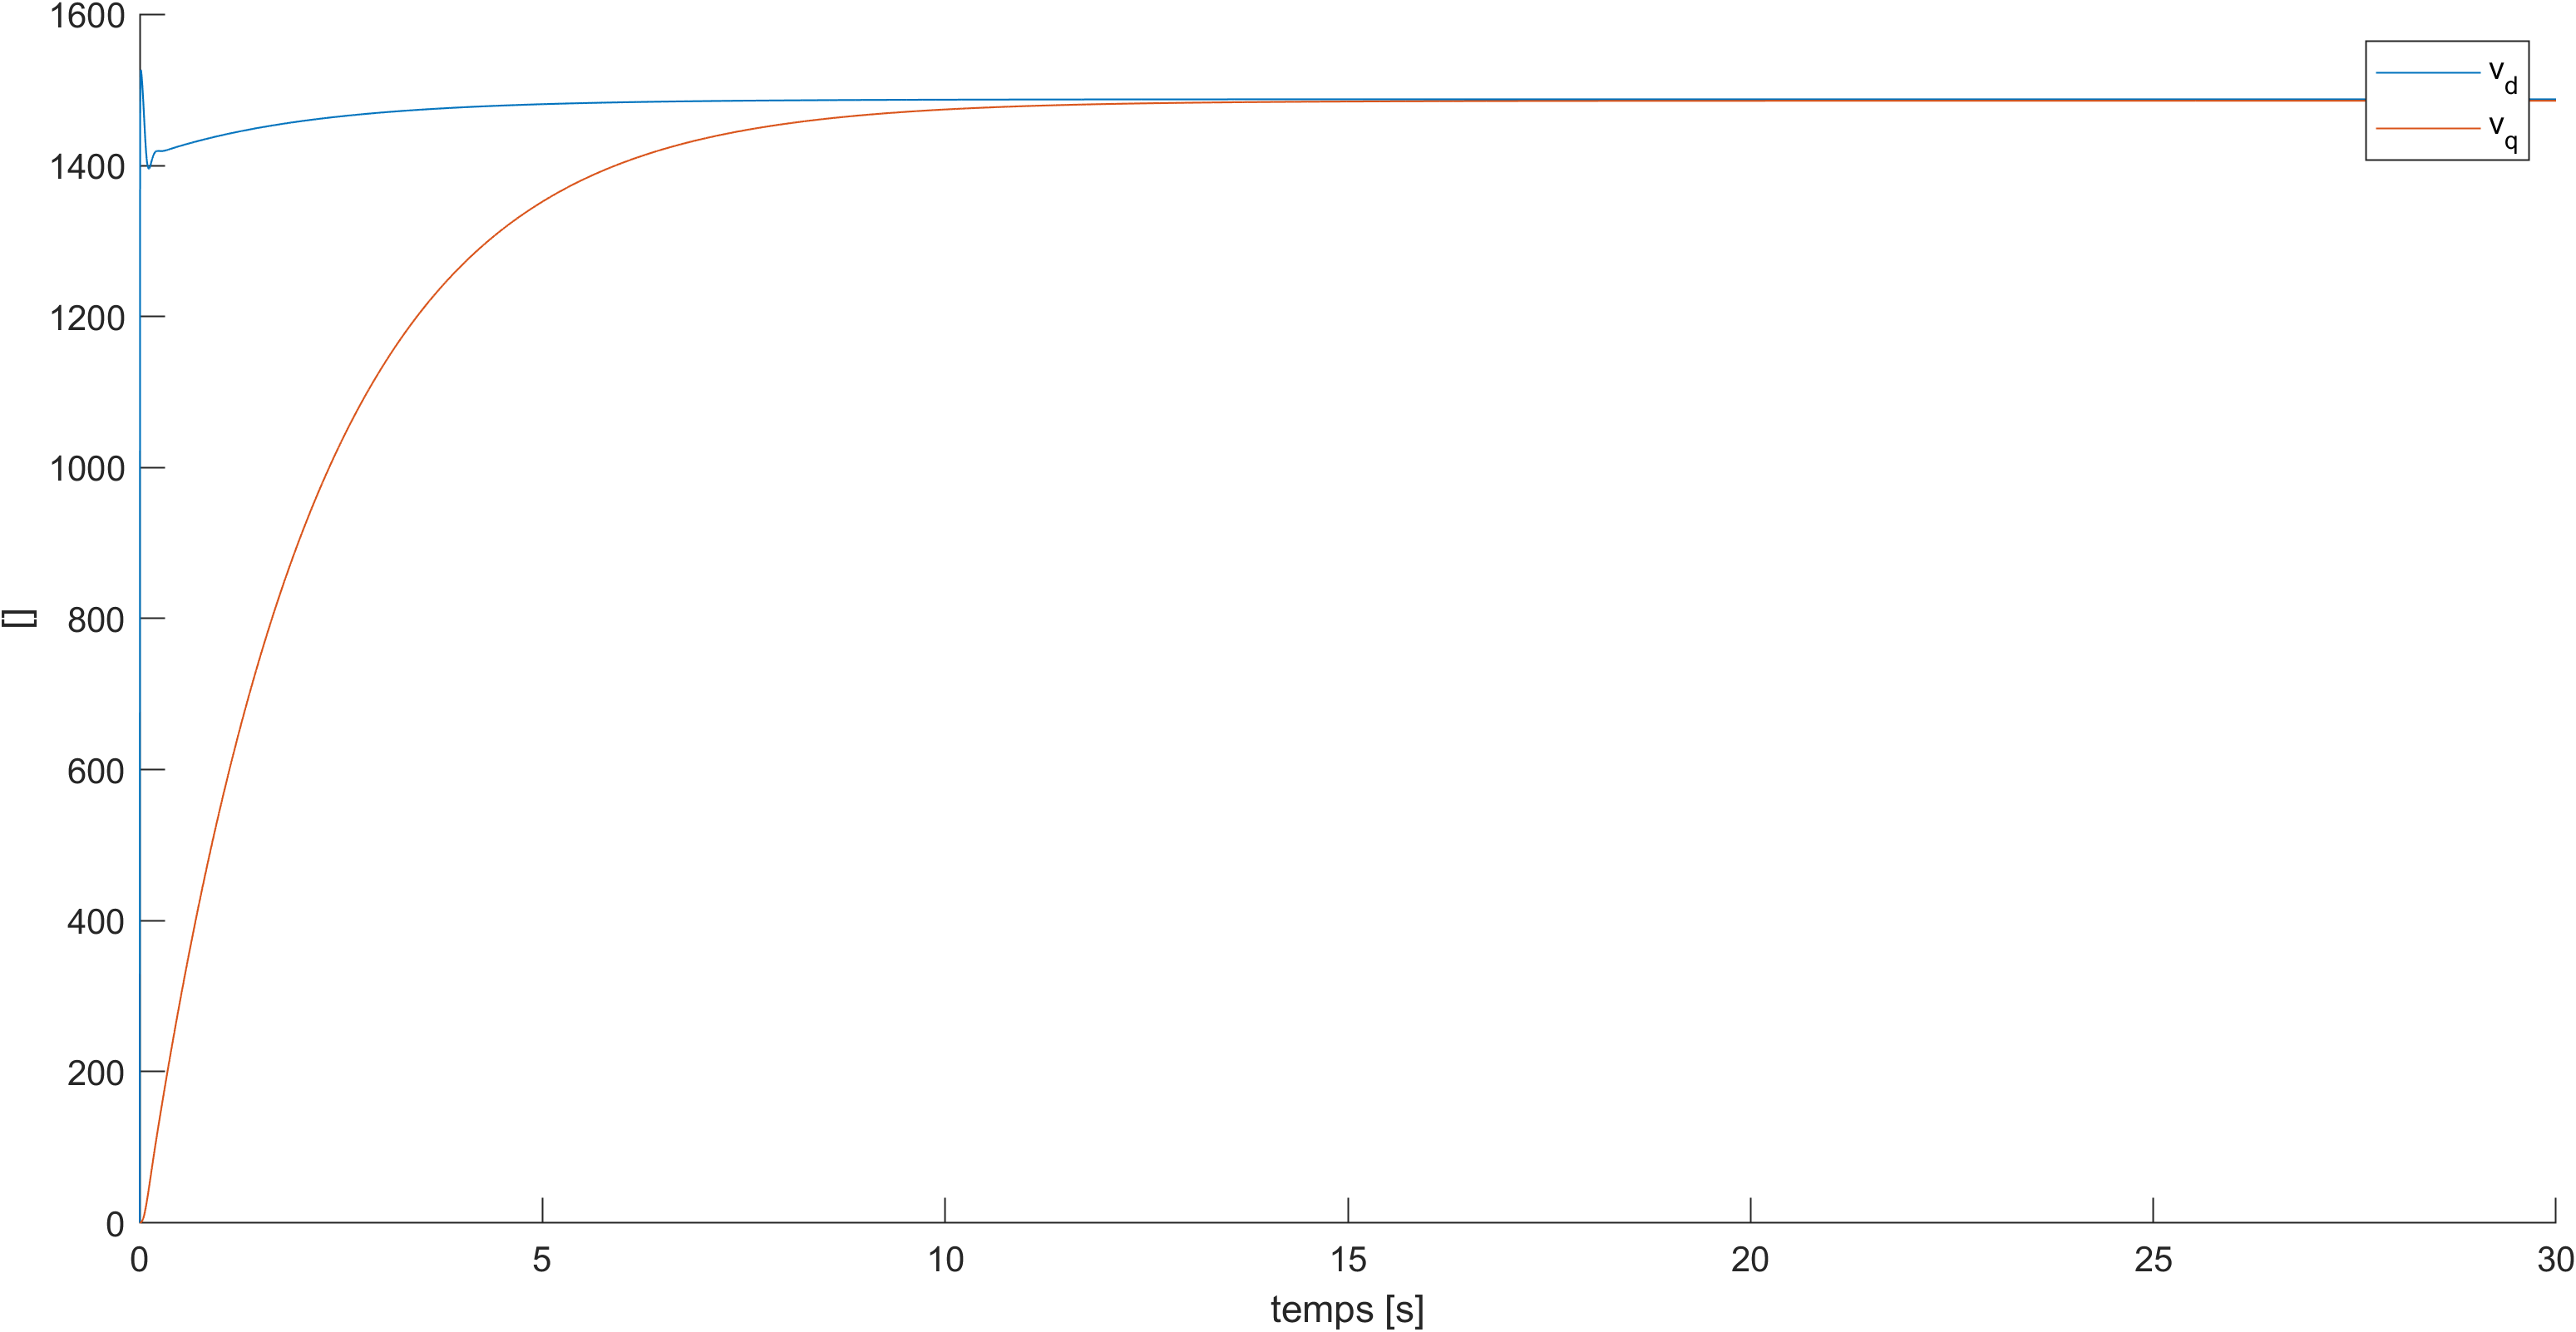
\includegraphics[width=0.8\textwidth]{simusMATLAB/MAS/comparation_wm.png} 
    \caption{Vérification de la évolution de la relation $\omega_m = \frac{C_e}{f}$ de la MAS.}
    \label{img-simuMatlab-comparation_wm}
\end{figure}


\begin{figure}[!h]
    \centering
    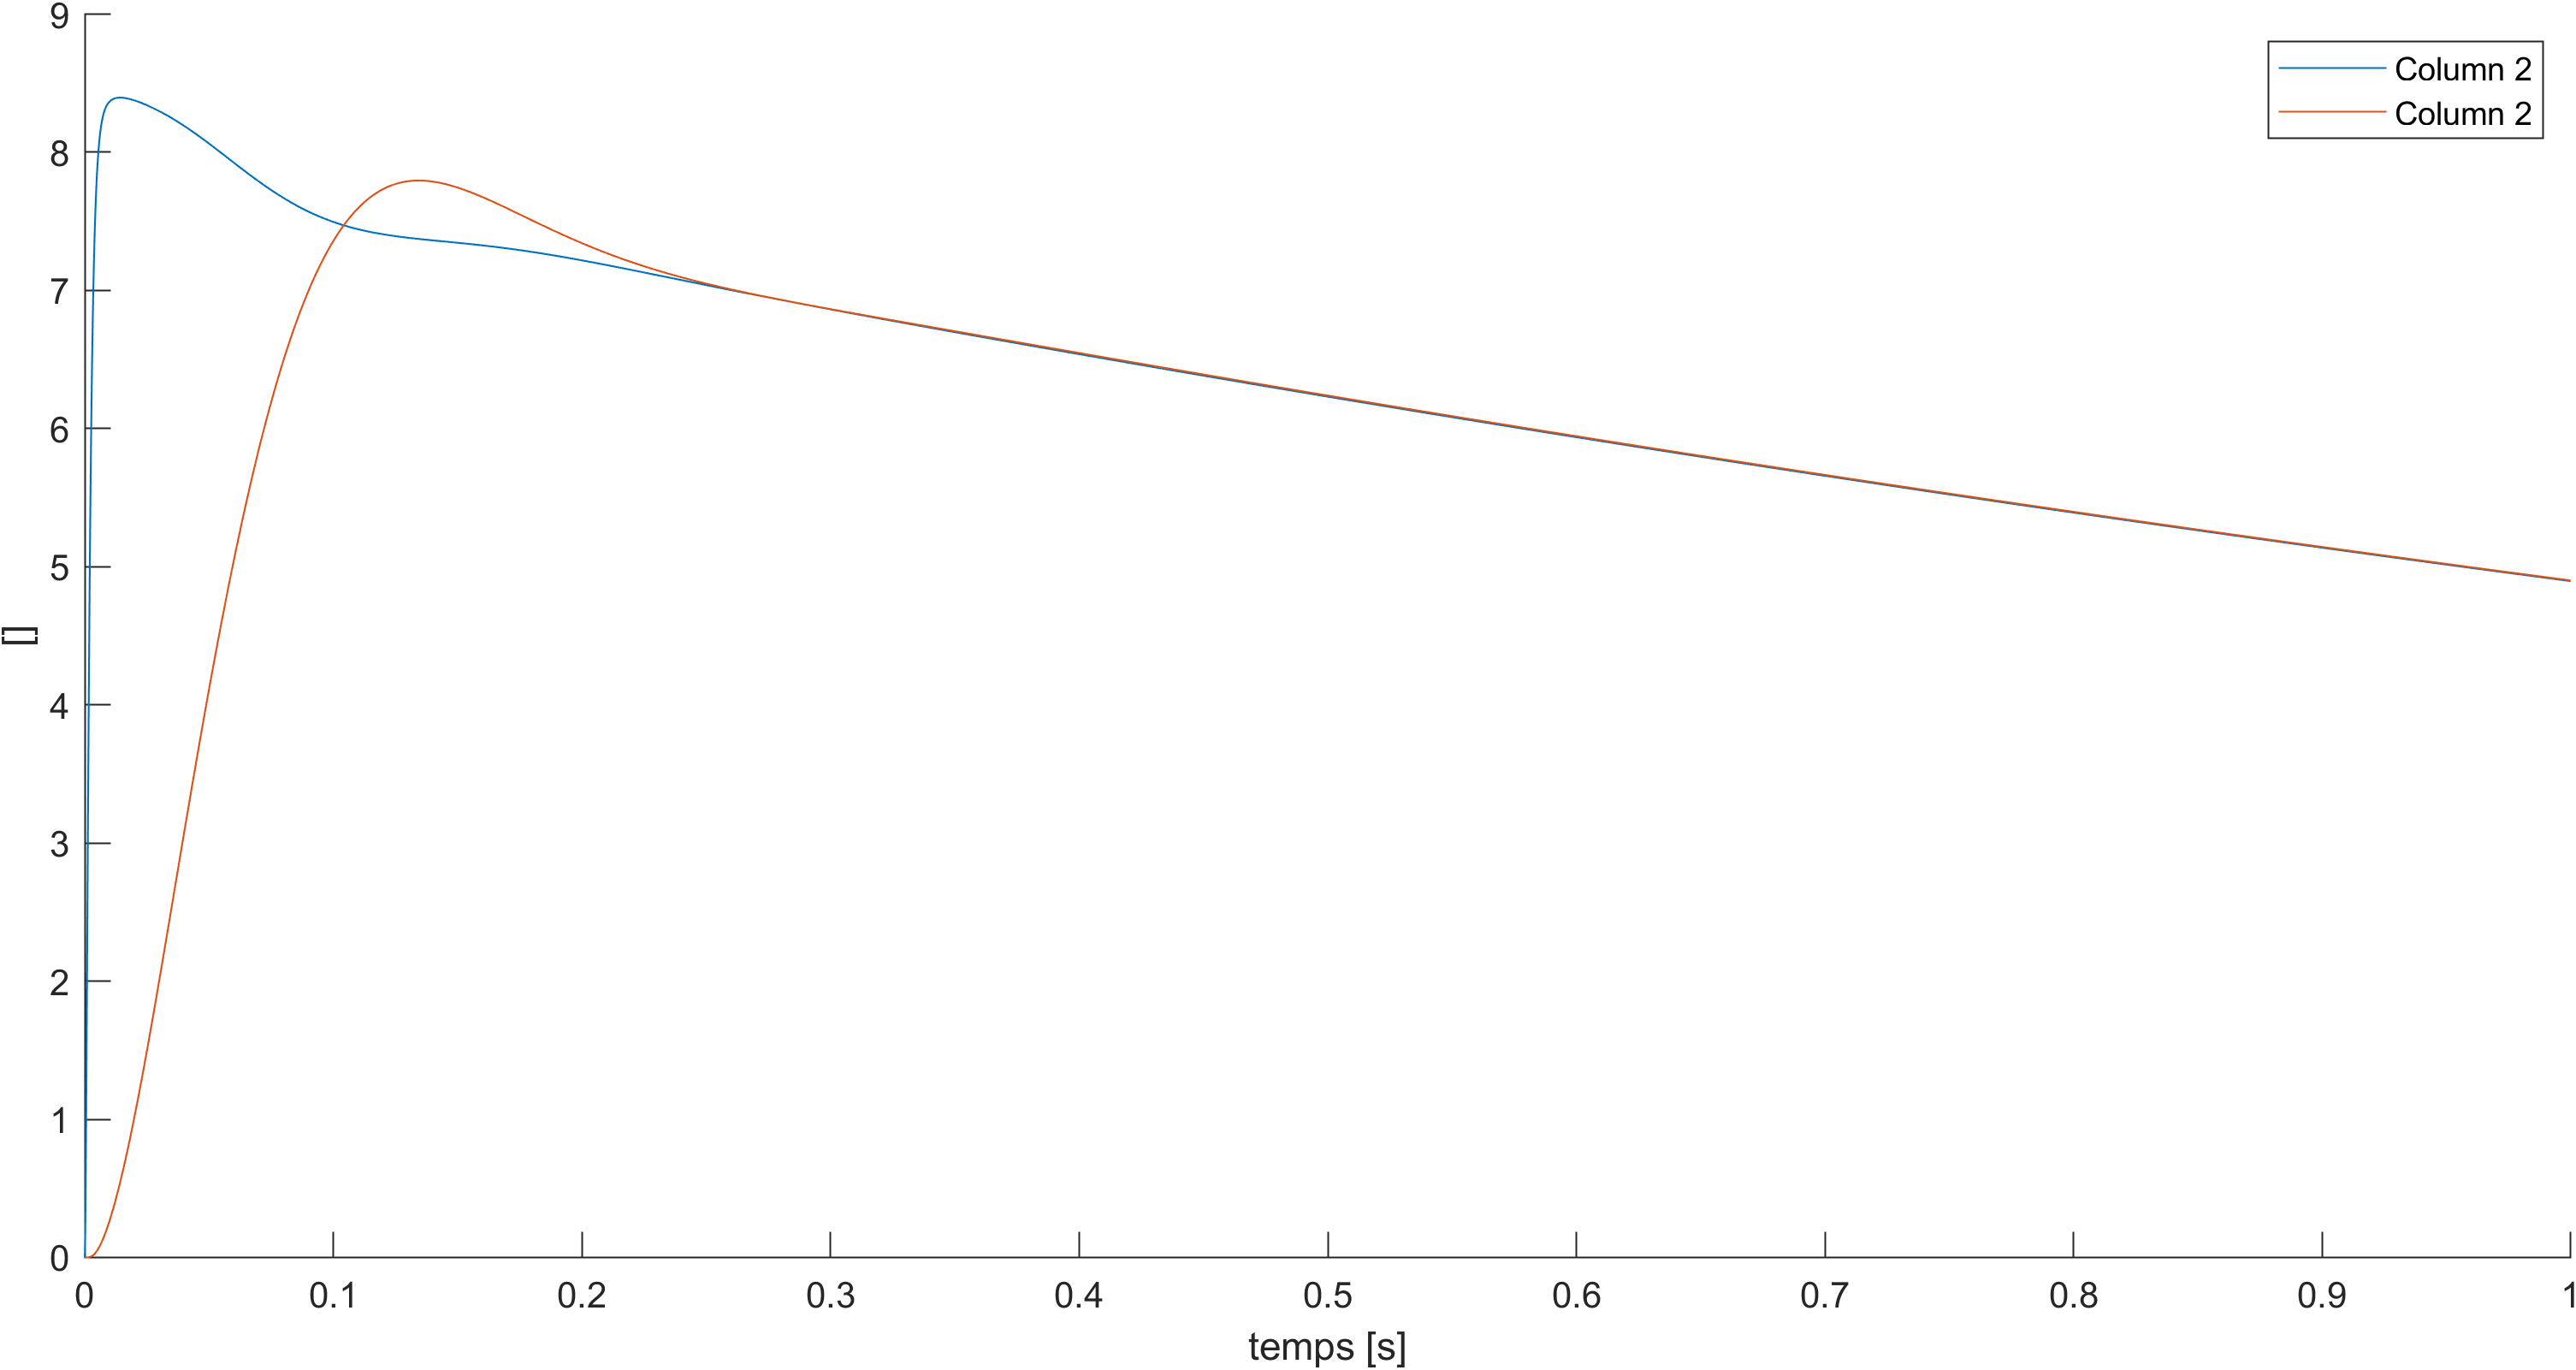
\includegraphics[width=0.8\textwidth]{simusMATLAB/MAS/relation.png} 
    \caption{Vérification de la évolution de la relation \ref{eq:dWm} de la MAS.}
    \label{img-simuMatlab-relation}
\end{figure}


%---------------------------------------
\FloatBarrier
\subsection{Simulation MADA}
%---------------------------------------

Afin de valider le modèle de la machine asynchrone de double alimentation les paramètres suivantes ont étés adoptés : $p = 2; R_s = 60 \cdot m\Omega; R_r = 38 m\Omega; L_s = L_{fs} + L_m, L_r = L_{fr} + L_m, \text{avec} L_m=12mH, L_{fr} = 180uH, \text{et} L_{fs}= 360uH; M_{sr} = L_m; f = -22 kg \cdot m^2 \cdot s^-1; J = 0.4 kg \cdot m^2$. Ces paramètres utilisées cherchent simuler une MADA qui opère comme génératrice éolienne. Dans cette machine simulée, au contraire de la MAS simulée précédemment, une charge de $5 \cdot 10^3 N\cdot m$ a été connecté, en plus du phénomène de frottement. 

En simulant d'abord la MADA agissant comme une machine asynchrone à induction, avec l'alimentation du rotor nulle, il est possible de vérifier son fonctionnement en observant la courbe de vitesse angulaire du rotor, qui présente un forte comportement oscillatoire dans sa démarrage mais que converge au valeur de $150 rad/s$ (Figure \ref{img-simuMADA-wm}). Pour ce première moment, fonctionnant comme moteur, la valeur de f a été changé à $0.1 kg \cdot m^2$. 


\begin{figure}[!h]
    \centering
    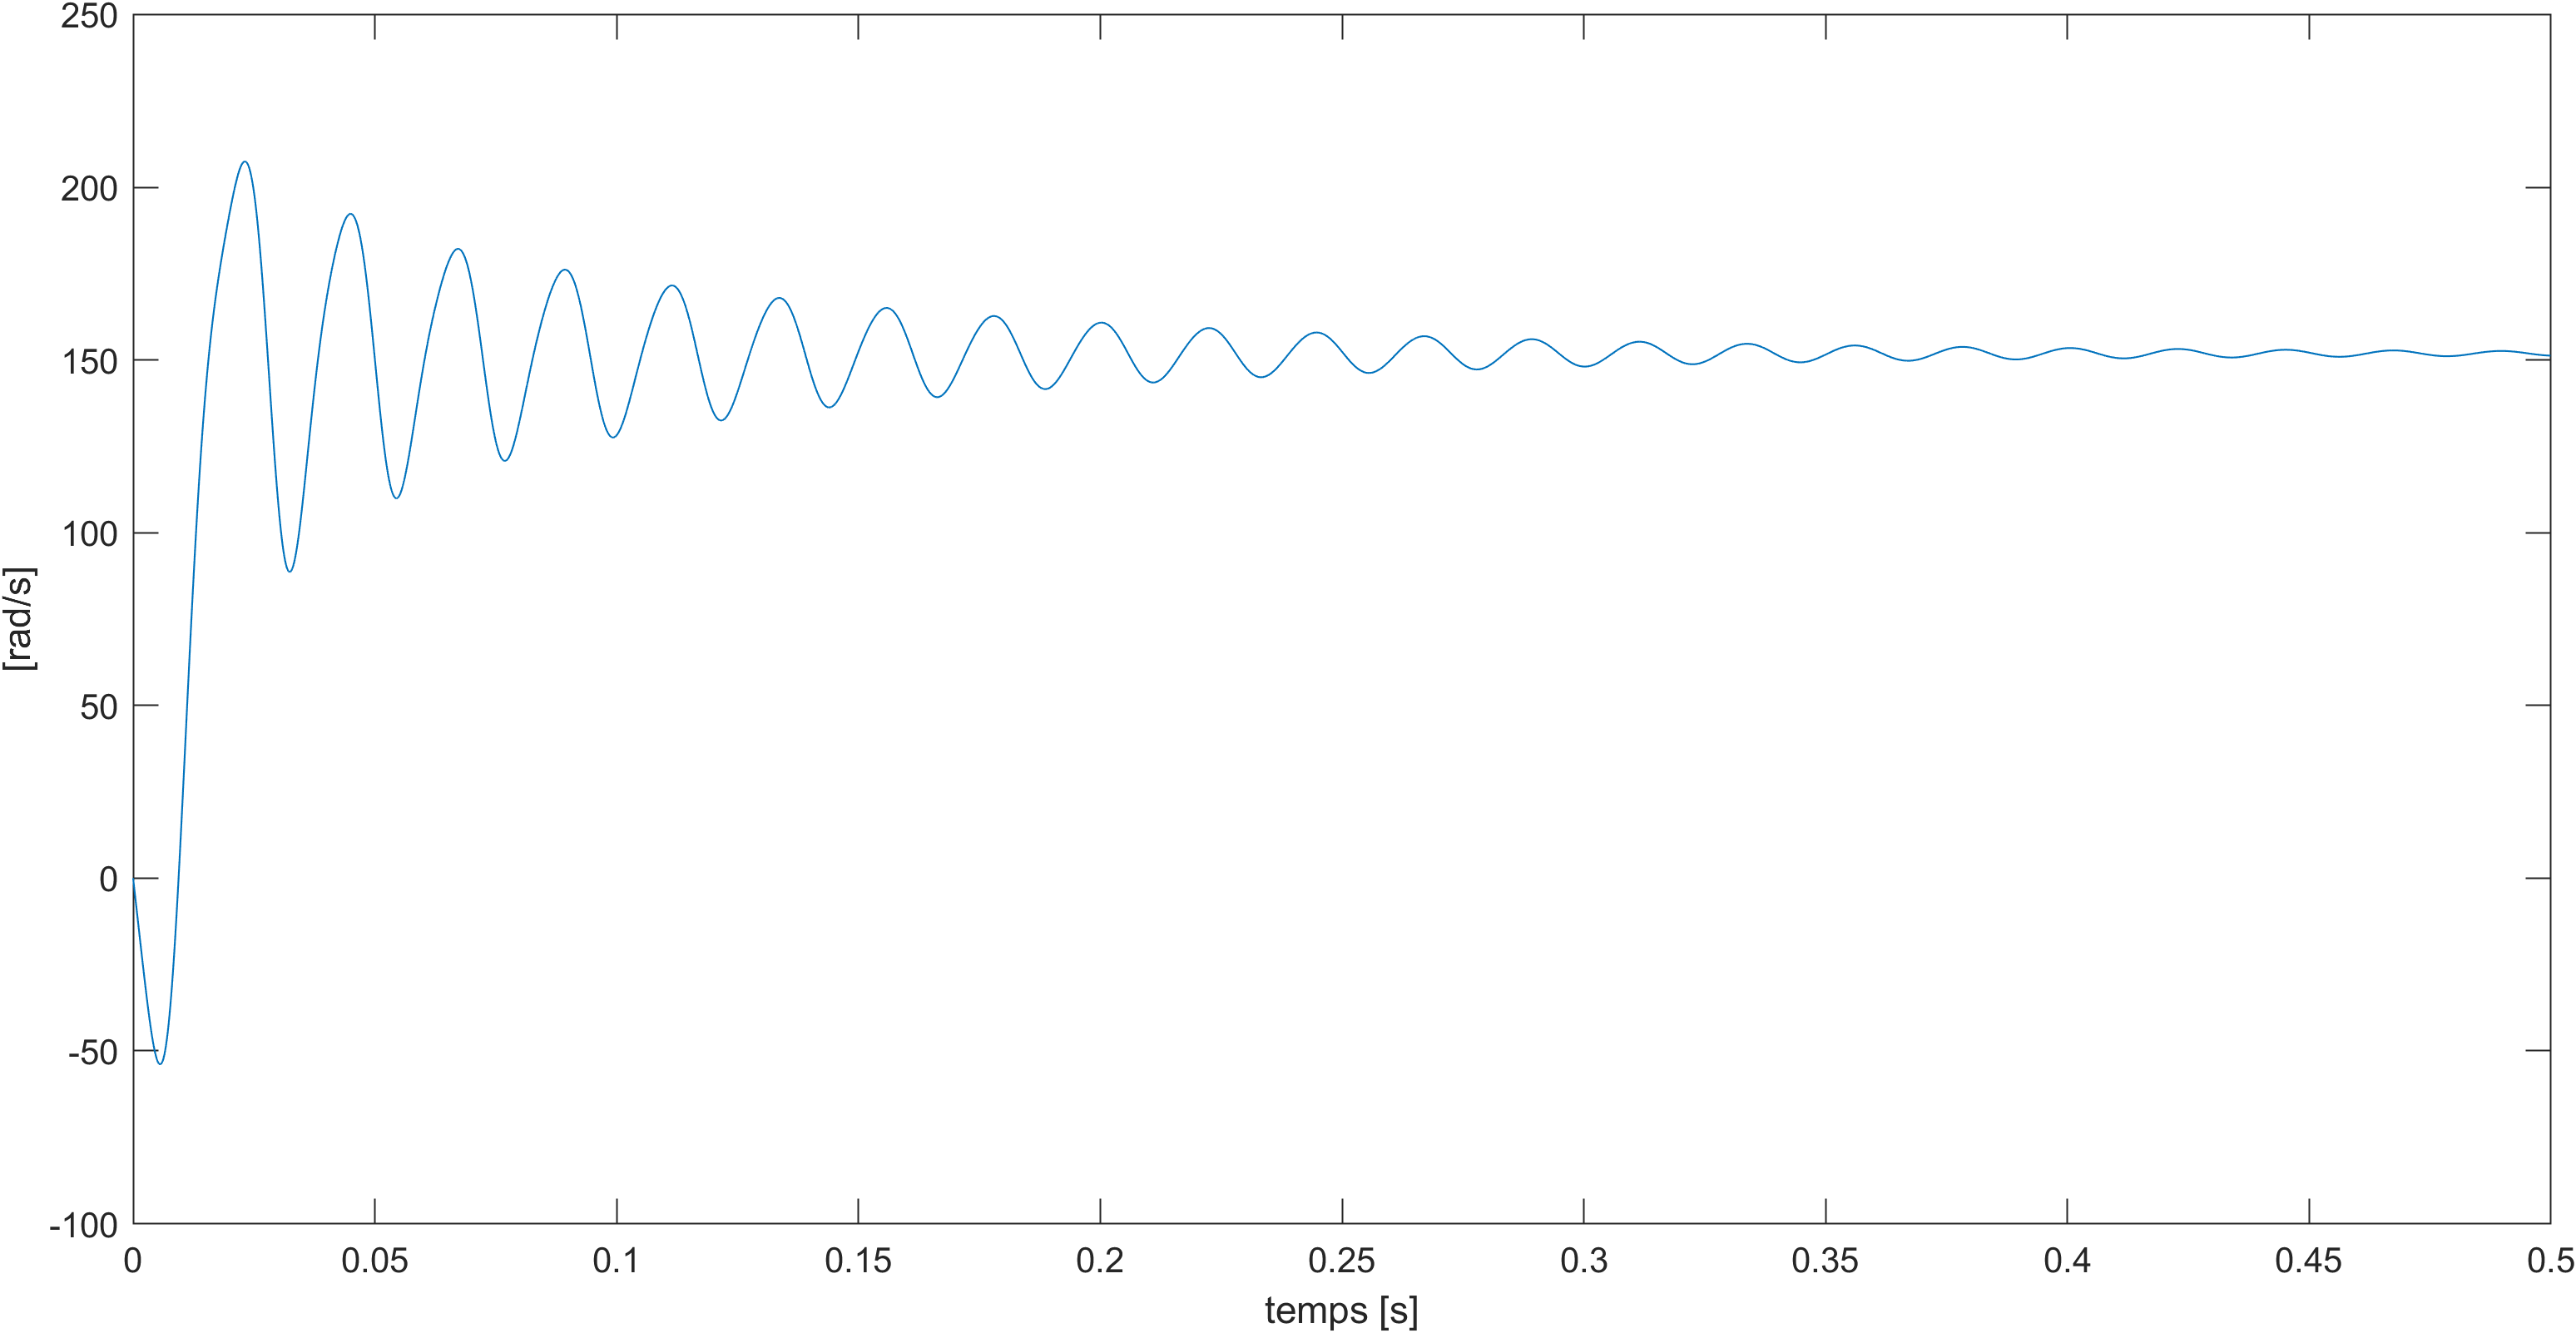
\includegraphics[width=0.8\textwidth]{simusMATLAB/MADA/wm.png} 
    \caption{Vitesse angulaire du rotor de la MADA mesurée au cous du temps.}
    \label{img-simuMADA-wm}
\end{figure}

Il est également possible de vérifier les valeurs de courant et de tension de la machine en cours de fonctionnement. La Figure \ref{img-simuMADA-ir_abc} montre le transitoire des courants triphasés dans le rotor de la machine, puis leur stabilisation en régime permanent. Il en va de même pour les figures \ref{img-simuMADA-ir_alphabeta} et \ref{img-simuMADA-is_abc}, où \ref{img-simuMADA-is_abc} met en évidence les courants triphasés transitoires dans le stator de la machine. 


\begin{figure}[!h]
    \centering
    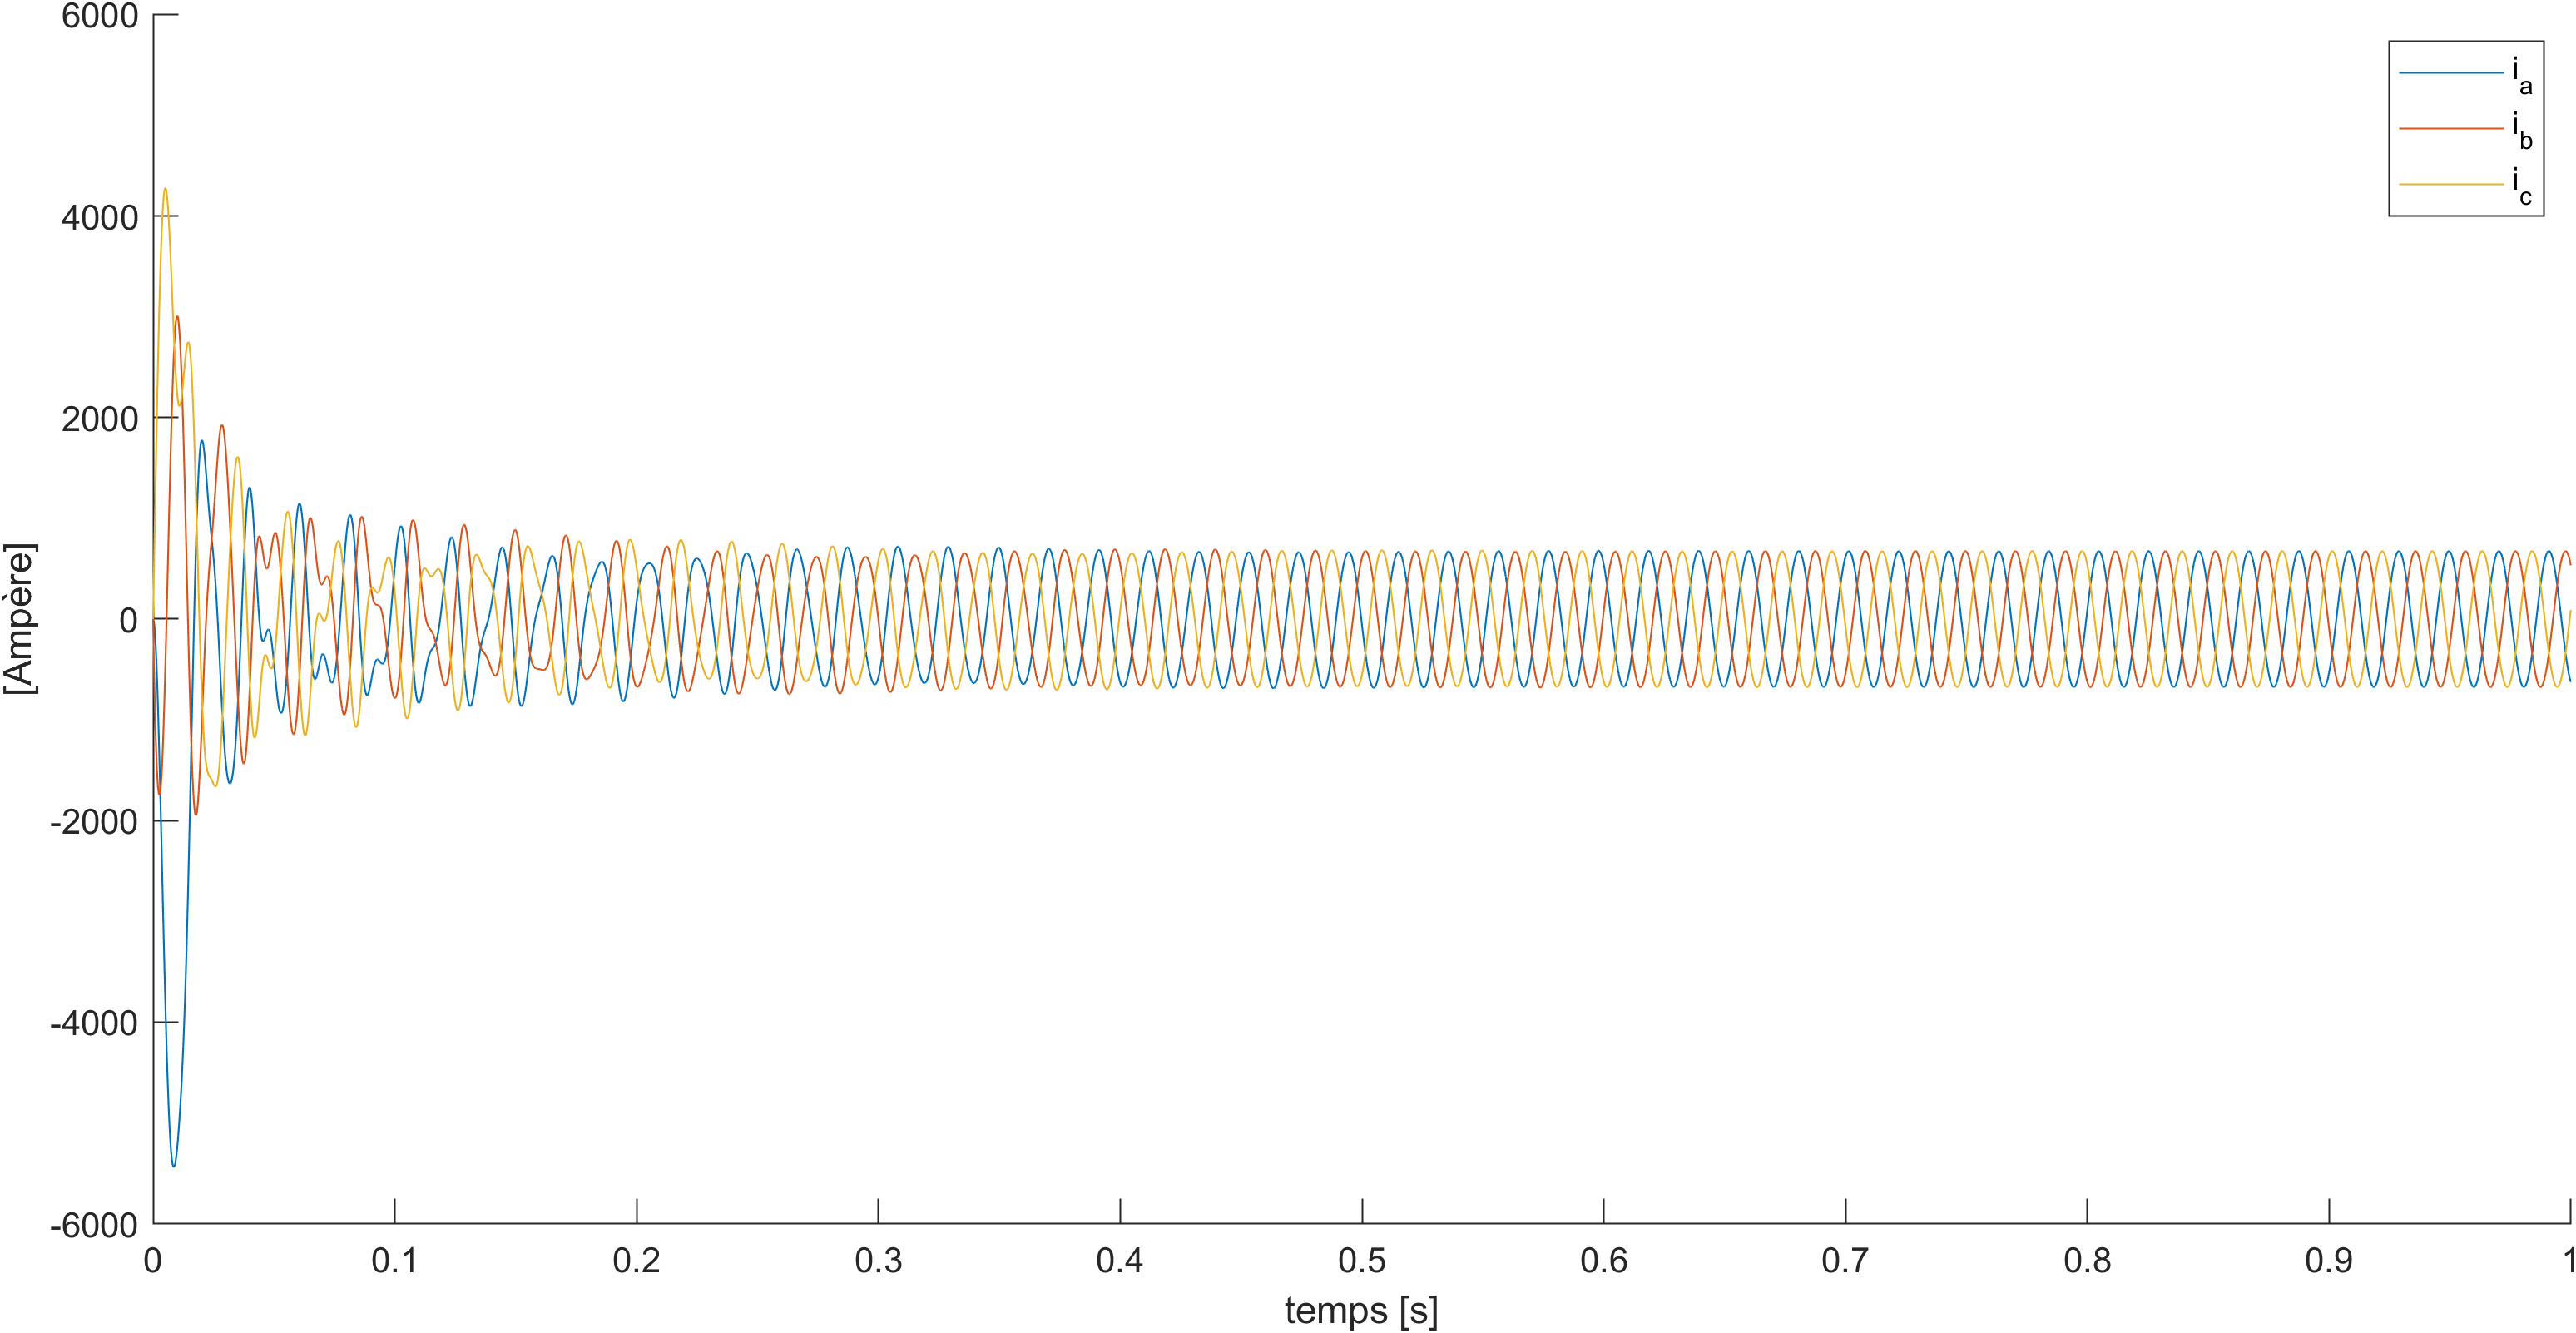
\includegraphics[width=0.8\textwidth]{simusMATLAB/MADA/ir_abc.png} 
    \caption{Courants rotoriques triphasées de la MADA mesurées au cous du temps.}
    \label{img-simuMADA-ir_abc}
\end{figure}


\begin{figure}[!h]
    \centering
    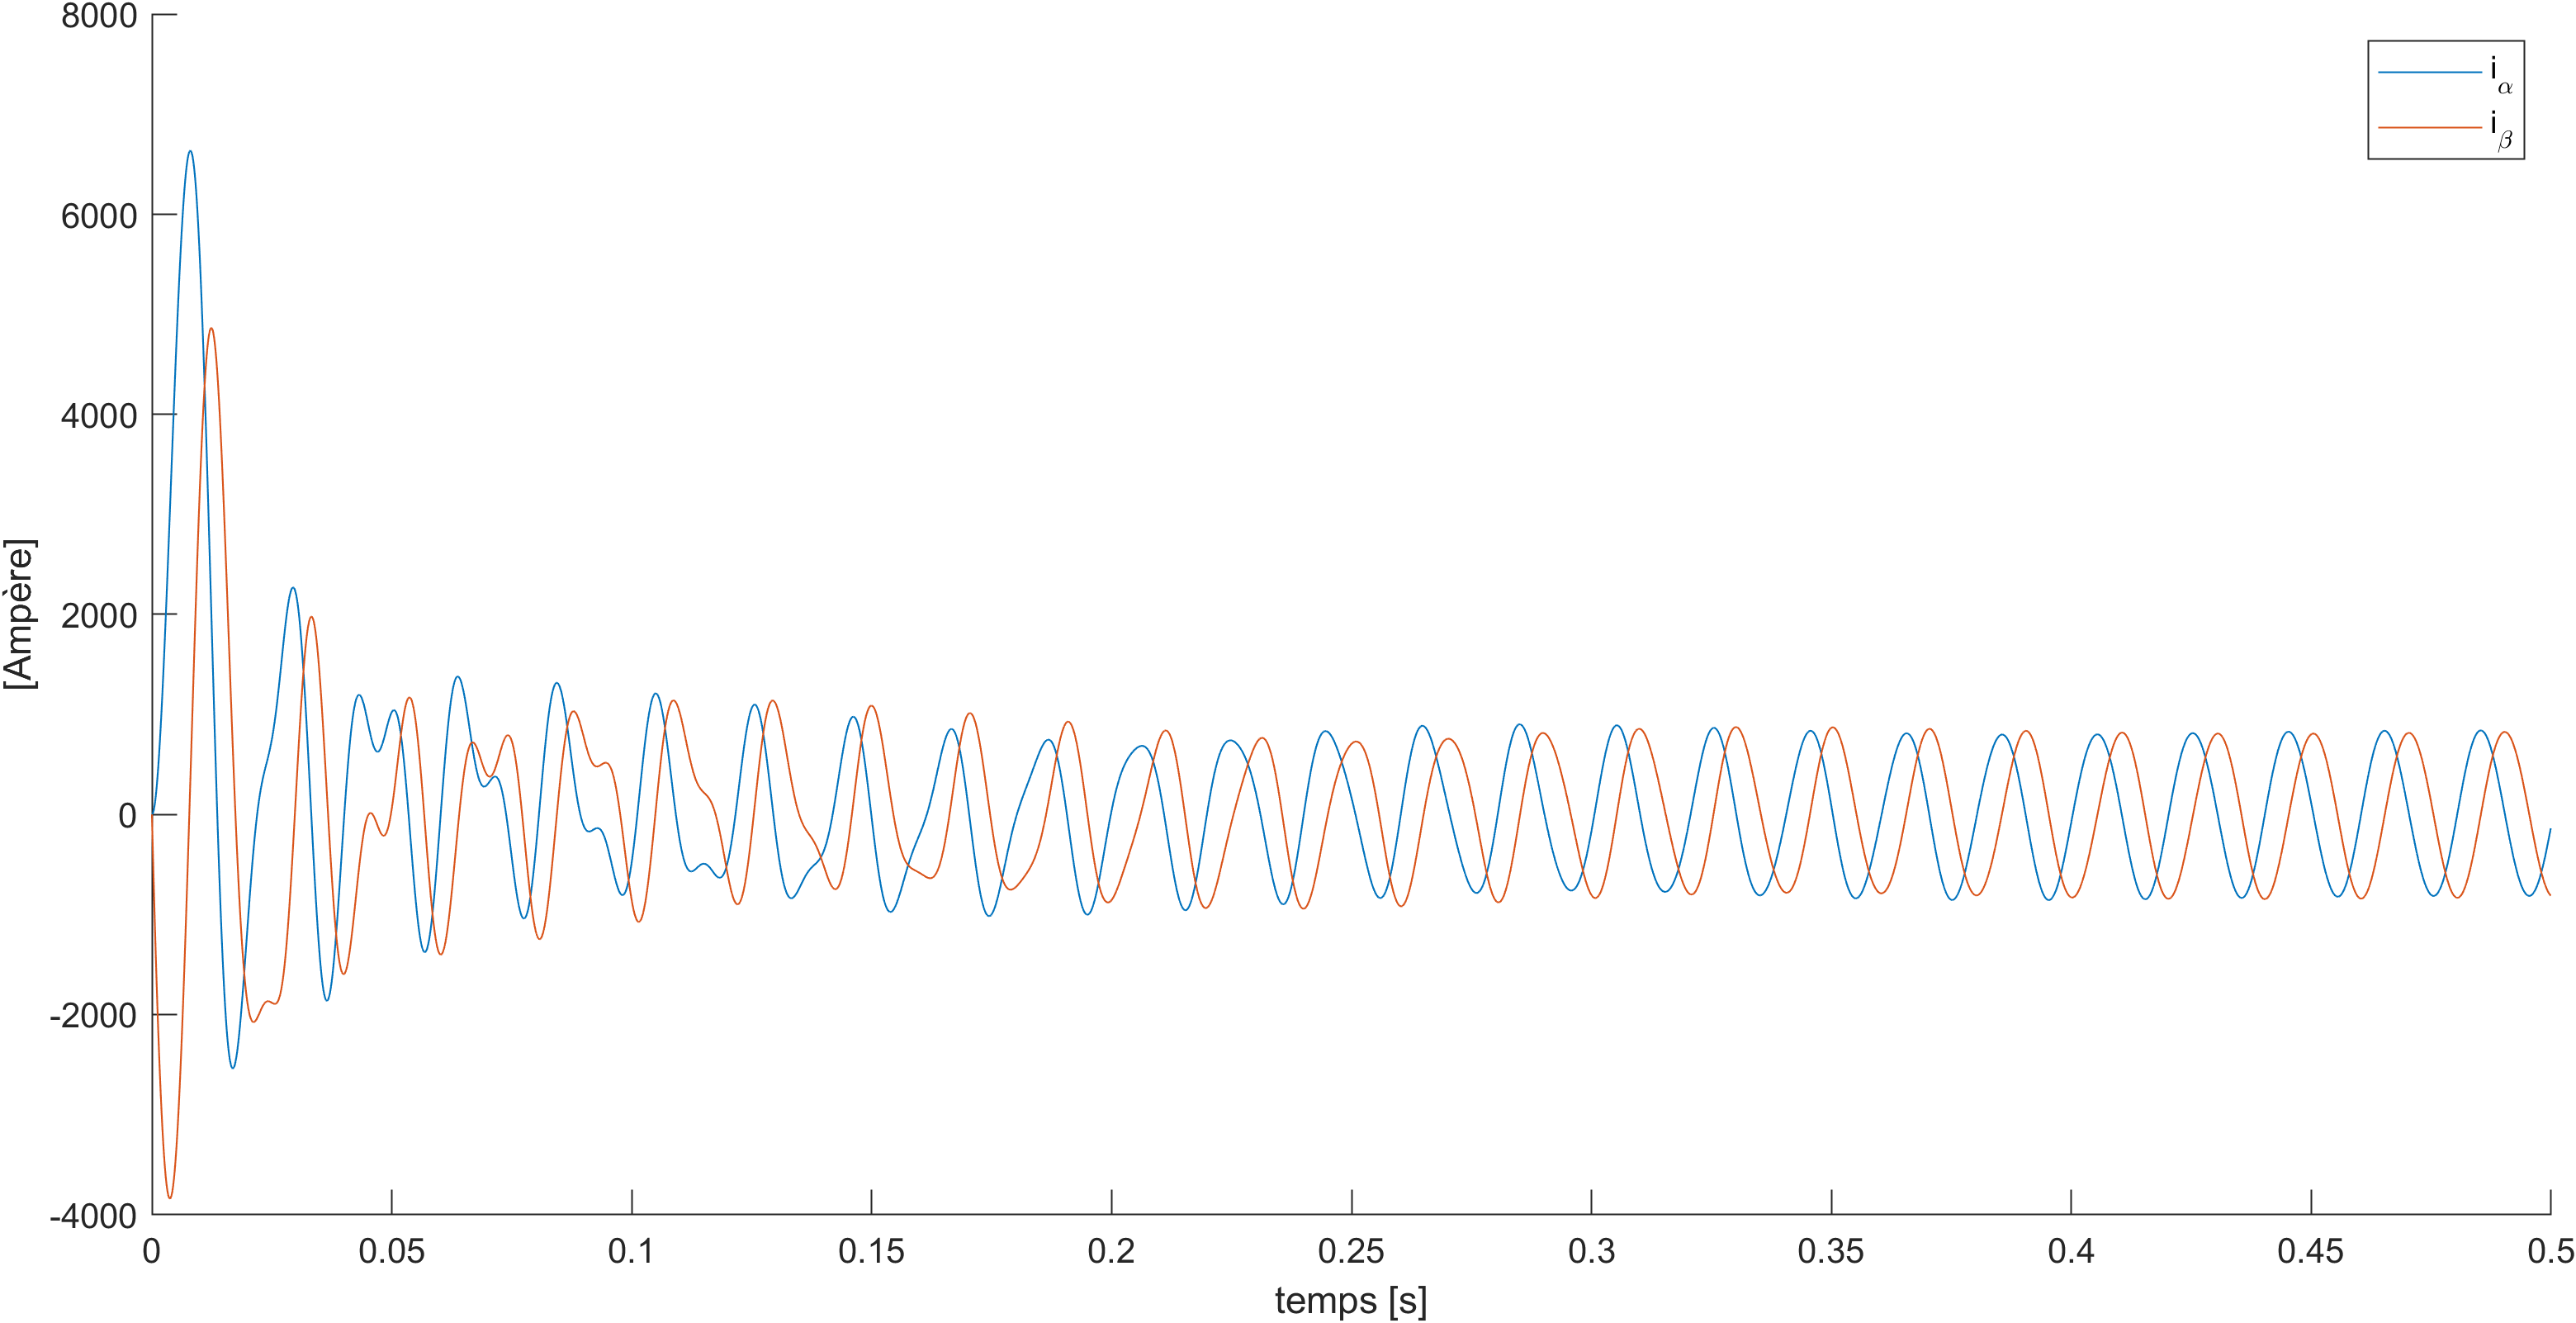
\includegraphics[width=0.8\textwidth]{simusMATLAB/MADA/ir_alphabeta.png} 
    \caption{Courants mesurées dans le repère $\alpha\beta$ de la MADA au long du temps.}
    \label{img-simuMADA-ir_alphabeta}
\end{figure}


\begin{figure}[!h]
    \centering
    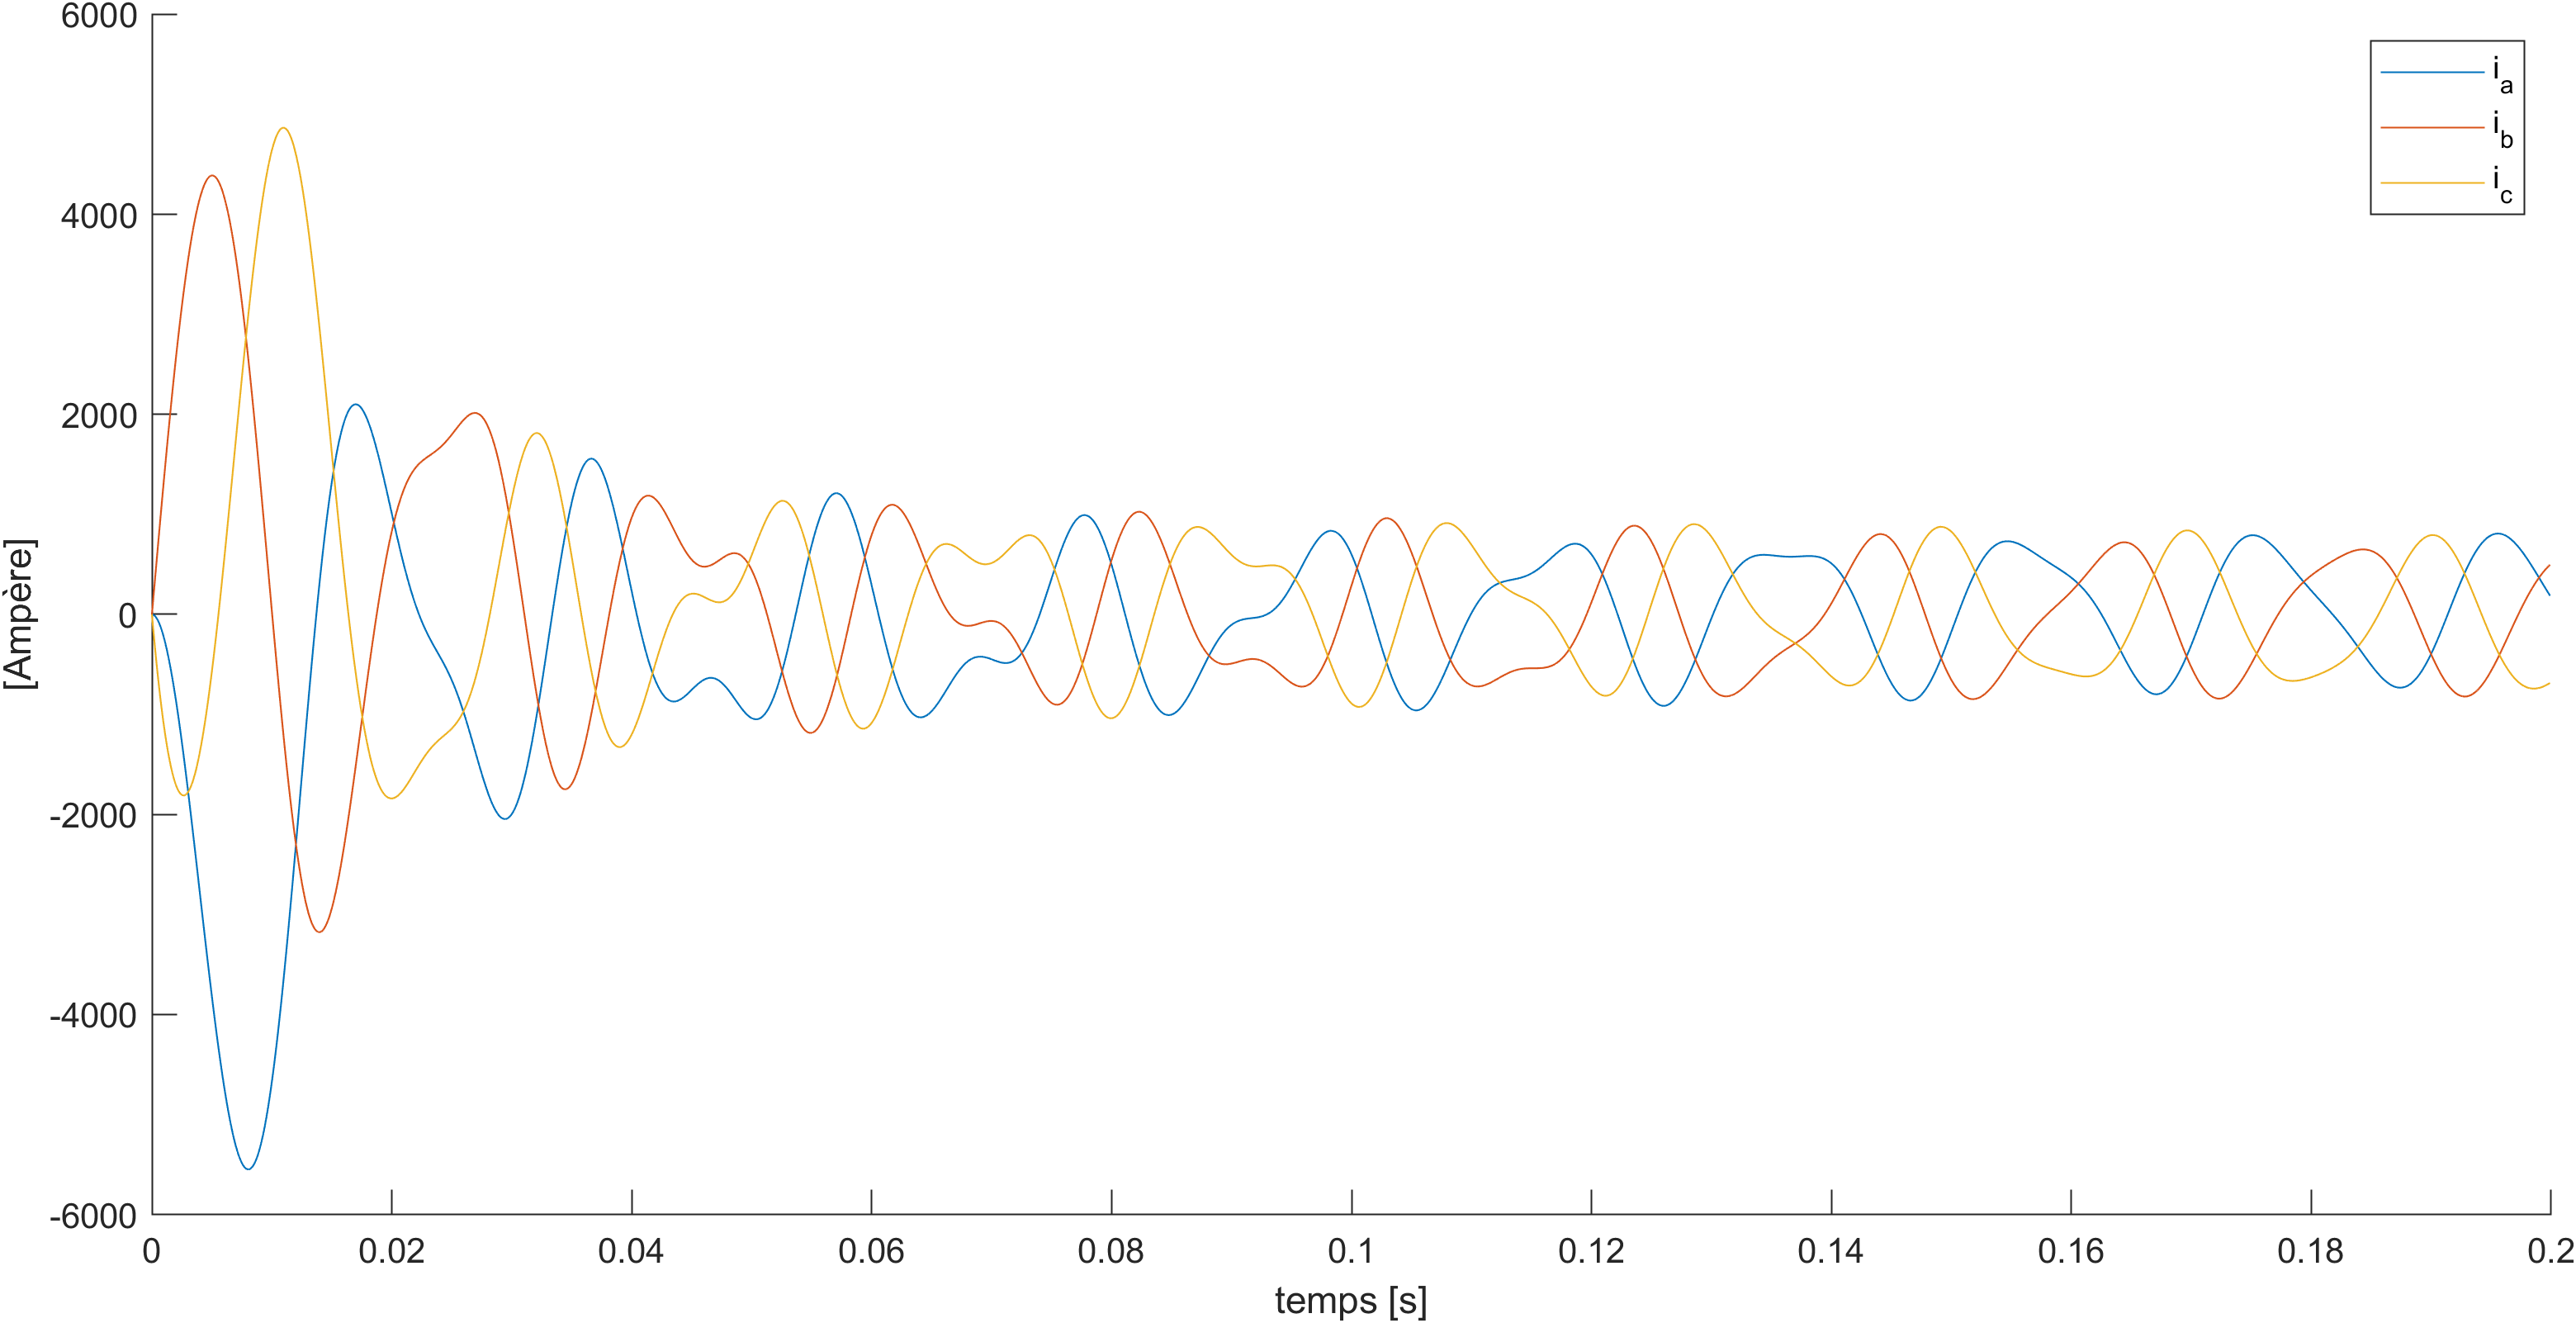
\includegraphics[width=0.8\textwidth]{simusMATLAB/MADA/is_abc.png} 
    \caption{Courants statoriques triphasées de la MADA mesurées au cous du temps.}
    \label{img-simuMADA-is_abc}
\end{figure}

En ce qui concerne les tensions mesurées pendant la simulation, les figures \ref{img-simuMADA-vs_abc} et \ref{img-simuMADA-vs_dq} montrent un comportement similaire aux simulations précédentes réalisées avec MAS, ce qui démontre l'efficacité des transformations de Park et de Concordia appliquées. La période transitoire et la stabilisation des flux à l'intérieur de la machine sont également visibles sur la Figure \ref{img-simuMADA-fluxes}.


\begin{figure}[!h]
    \centering
    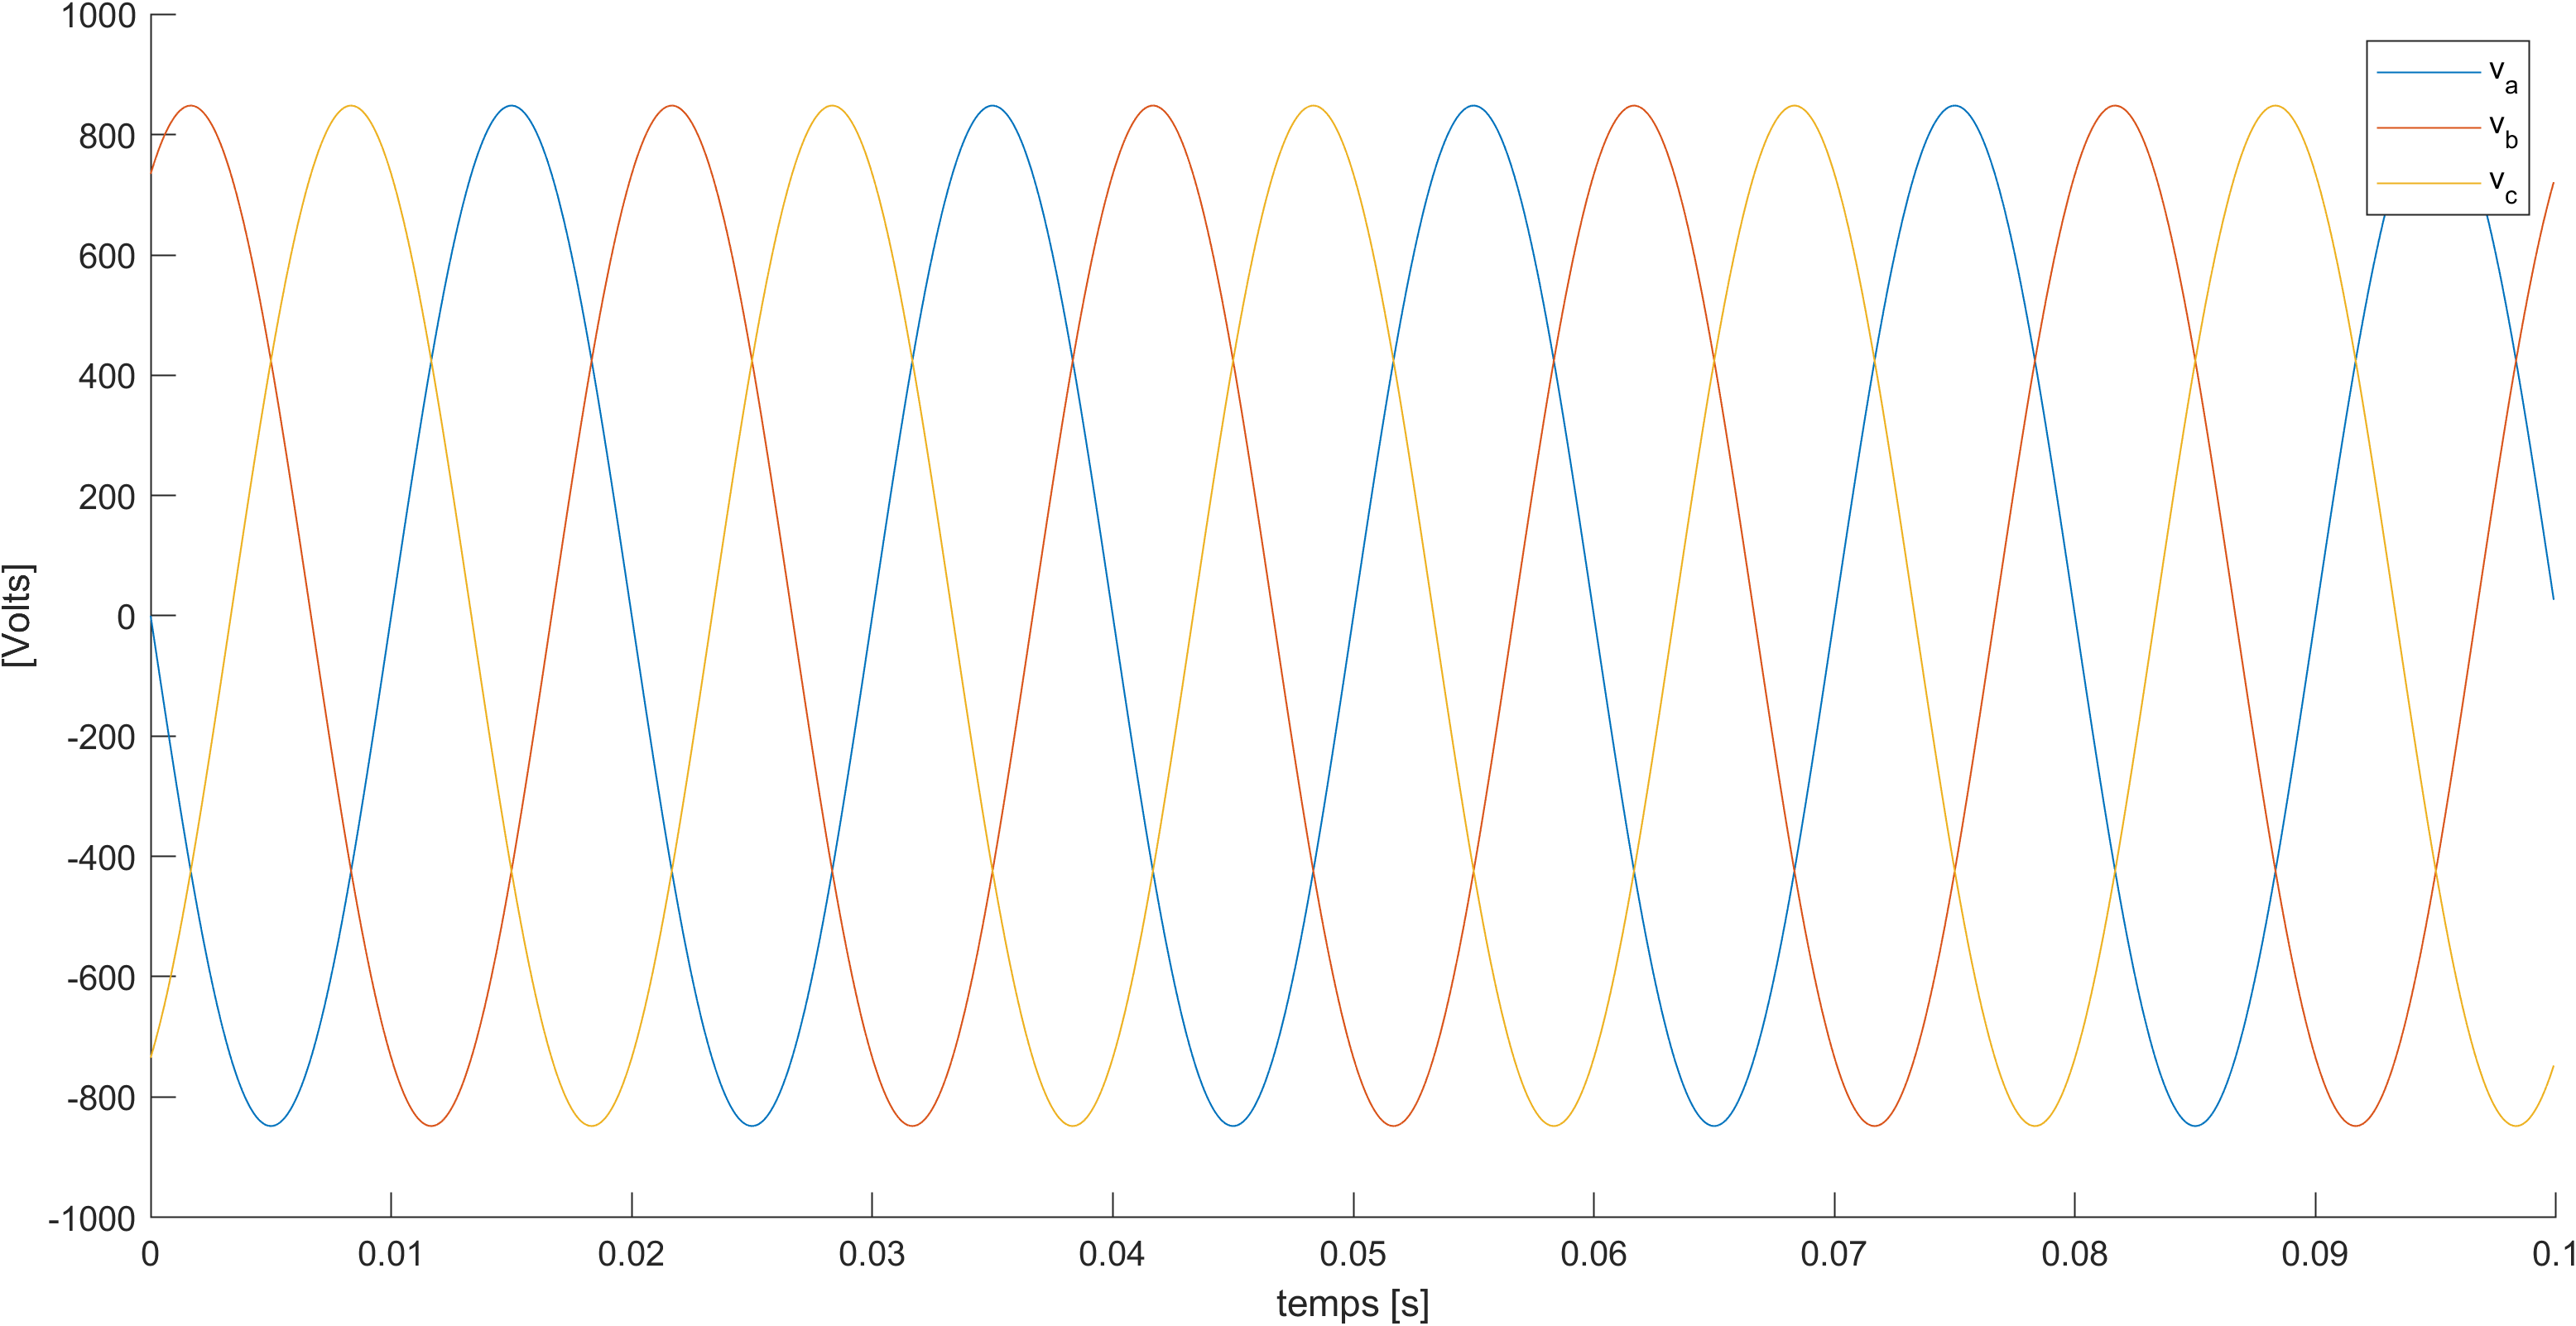
\includegraphics[width=0.8\textwidth]{simusMATLAB/MADA/vs_abc.png} 
    \caption{Tensions statoriques triphasées de la MADA mesurées au cours du temps.}
    \label{img-simuMADA-vs_abc}
\end{figure}


\begin{figure}[!h]
    \centering
    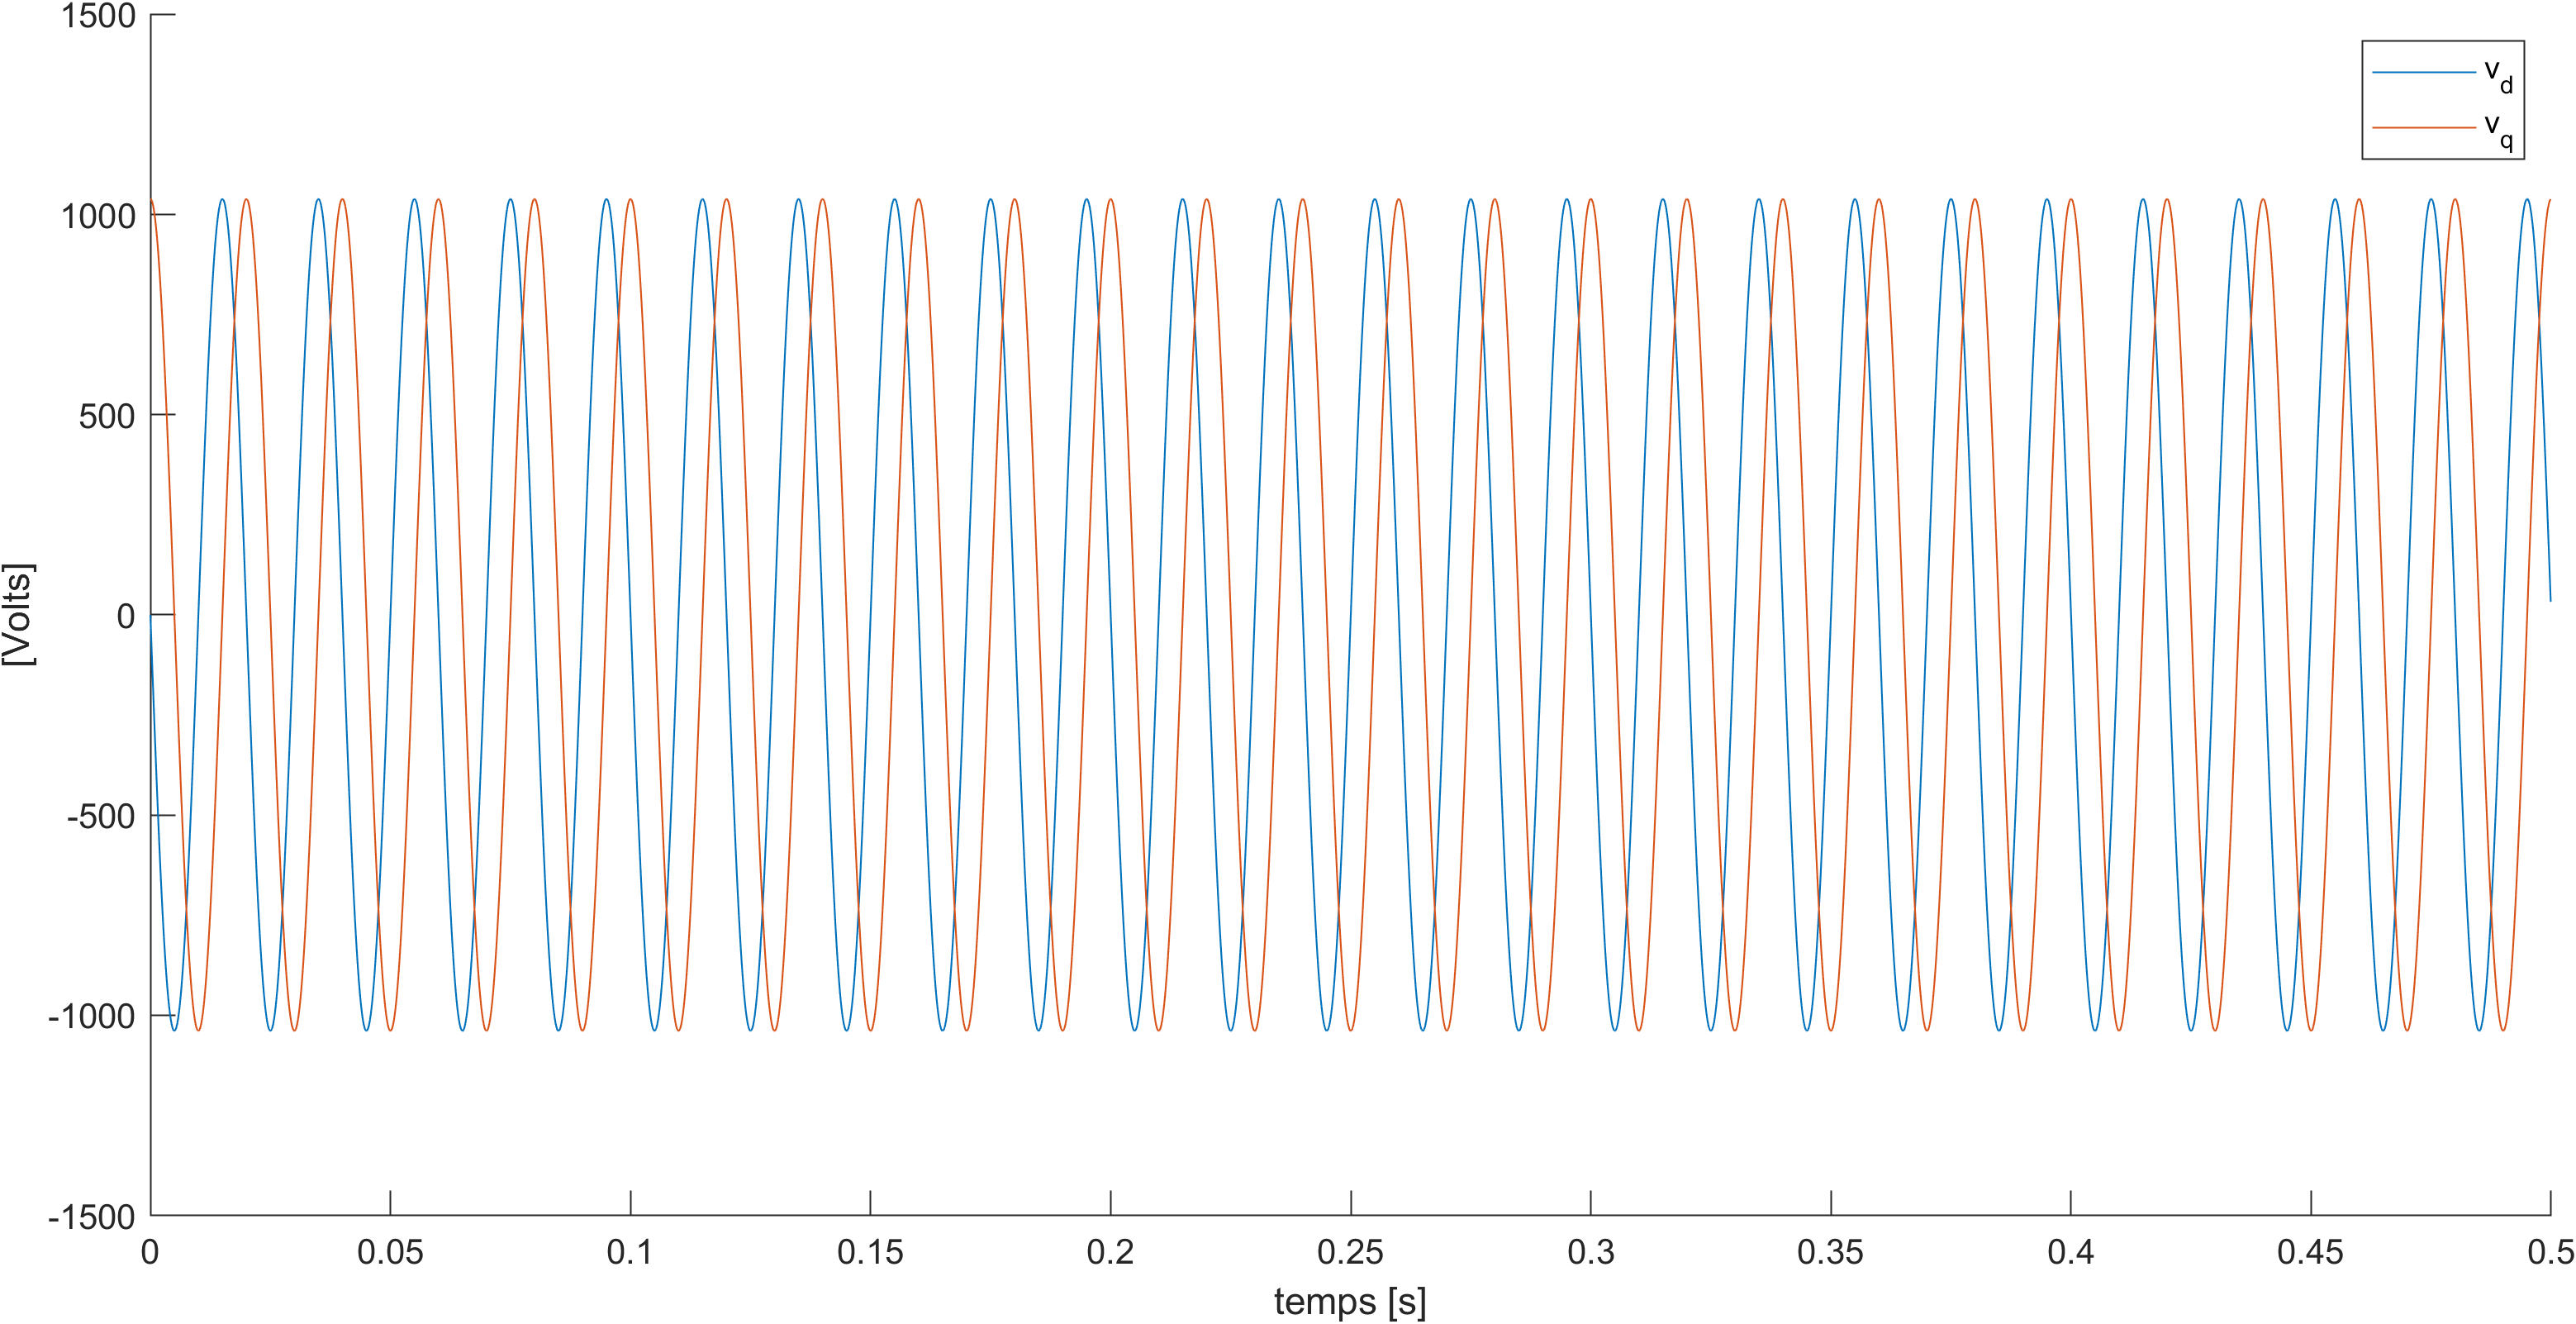
\includegraphics[width=0.8\textwidth]{simusMATLAB/MADA/vs_dq.png} 
    \caption{Tensions statoriques dq de la MADA mesurées au cours du temps.}
    \label{img-simuMADA-vs_dq}
\end{figure}


\begin{figure}[!h]
    \centering
    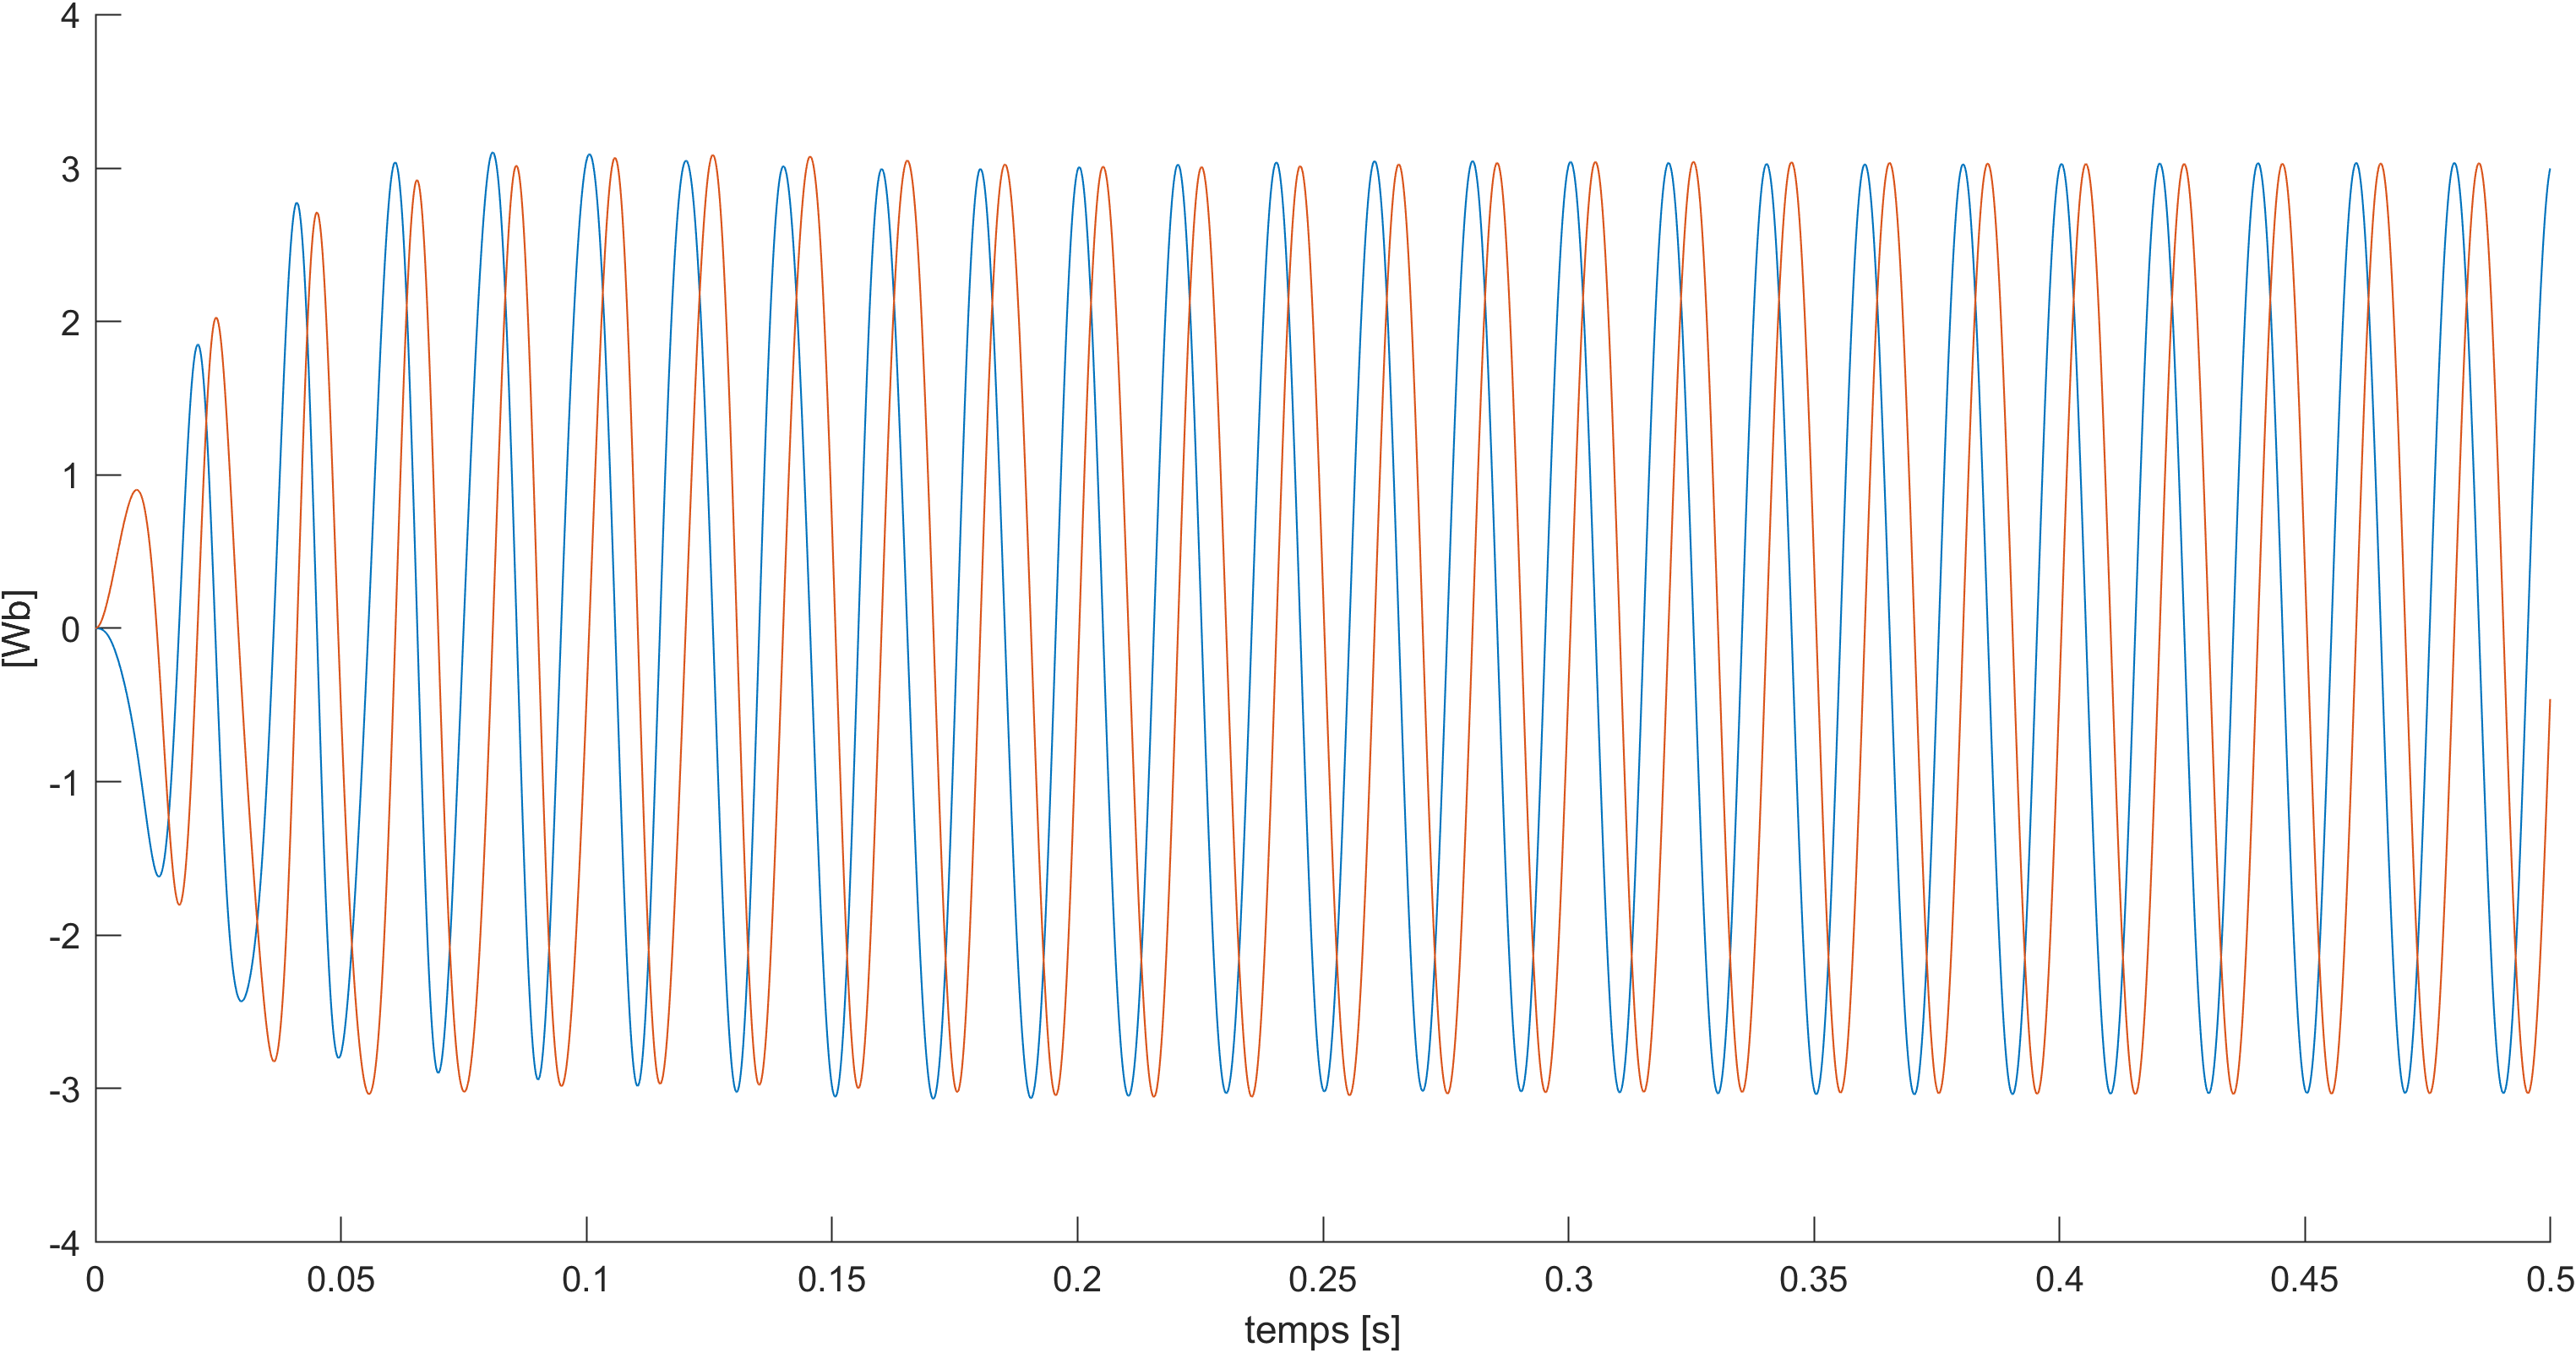
\includegraphics[width=0.8\textwidth]{simusMATLAB/MADA/fluxes.png} 
    \caption{Fluxes dq de la MADA mesurées au cours du temps.}
    \label{img-simuMADA-fluxes}
\end{figure}


En ce qui concerne le couple de la machine, sa puissance et couple, d'après les figures \ref{img-simuMADA-Ce}, \ref{img-simuMADA-P} et \ref{img-simuMADA-torque} respectivement, de fortes oscillations ont été constatées dans son régime transitoire jusqu'à ce qu'il se stabilise aux valeurs respectives de plateau.


\begin{figure}[!h]
    \centering
    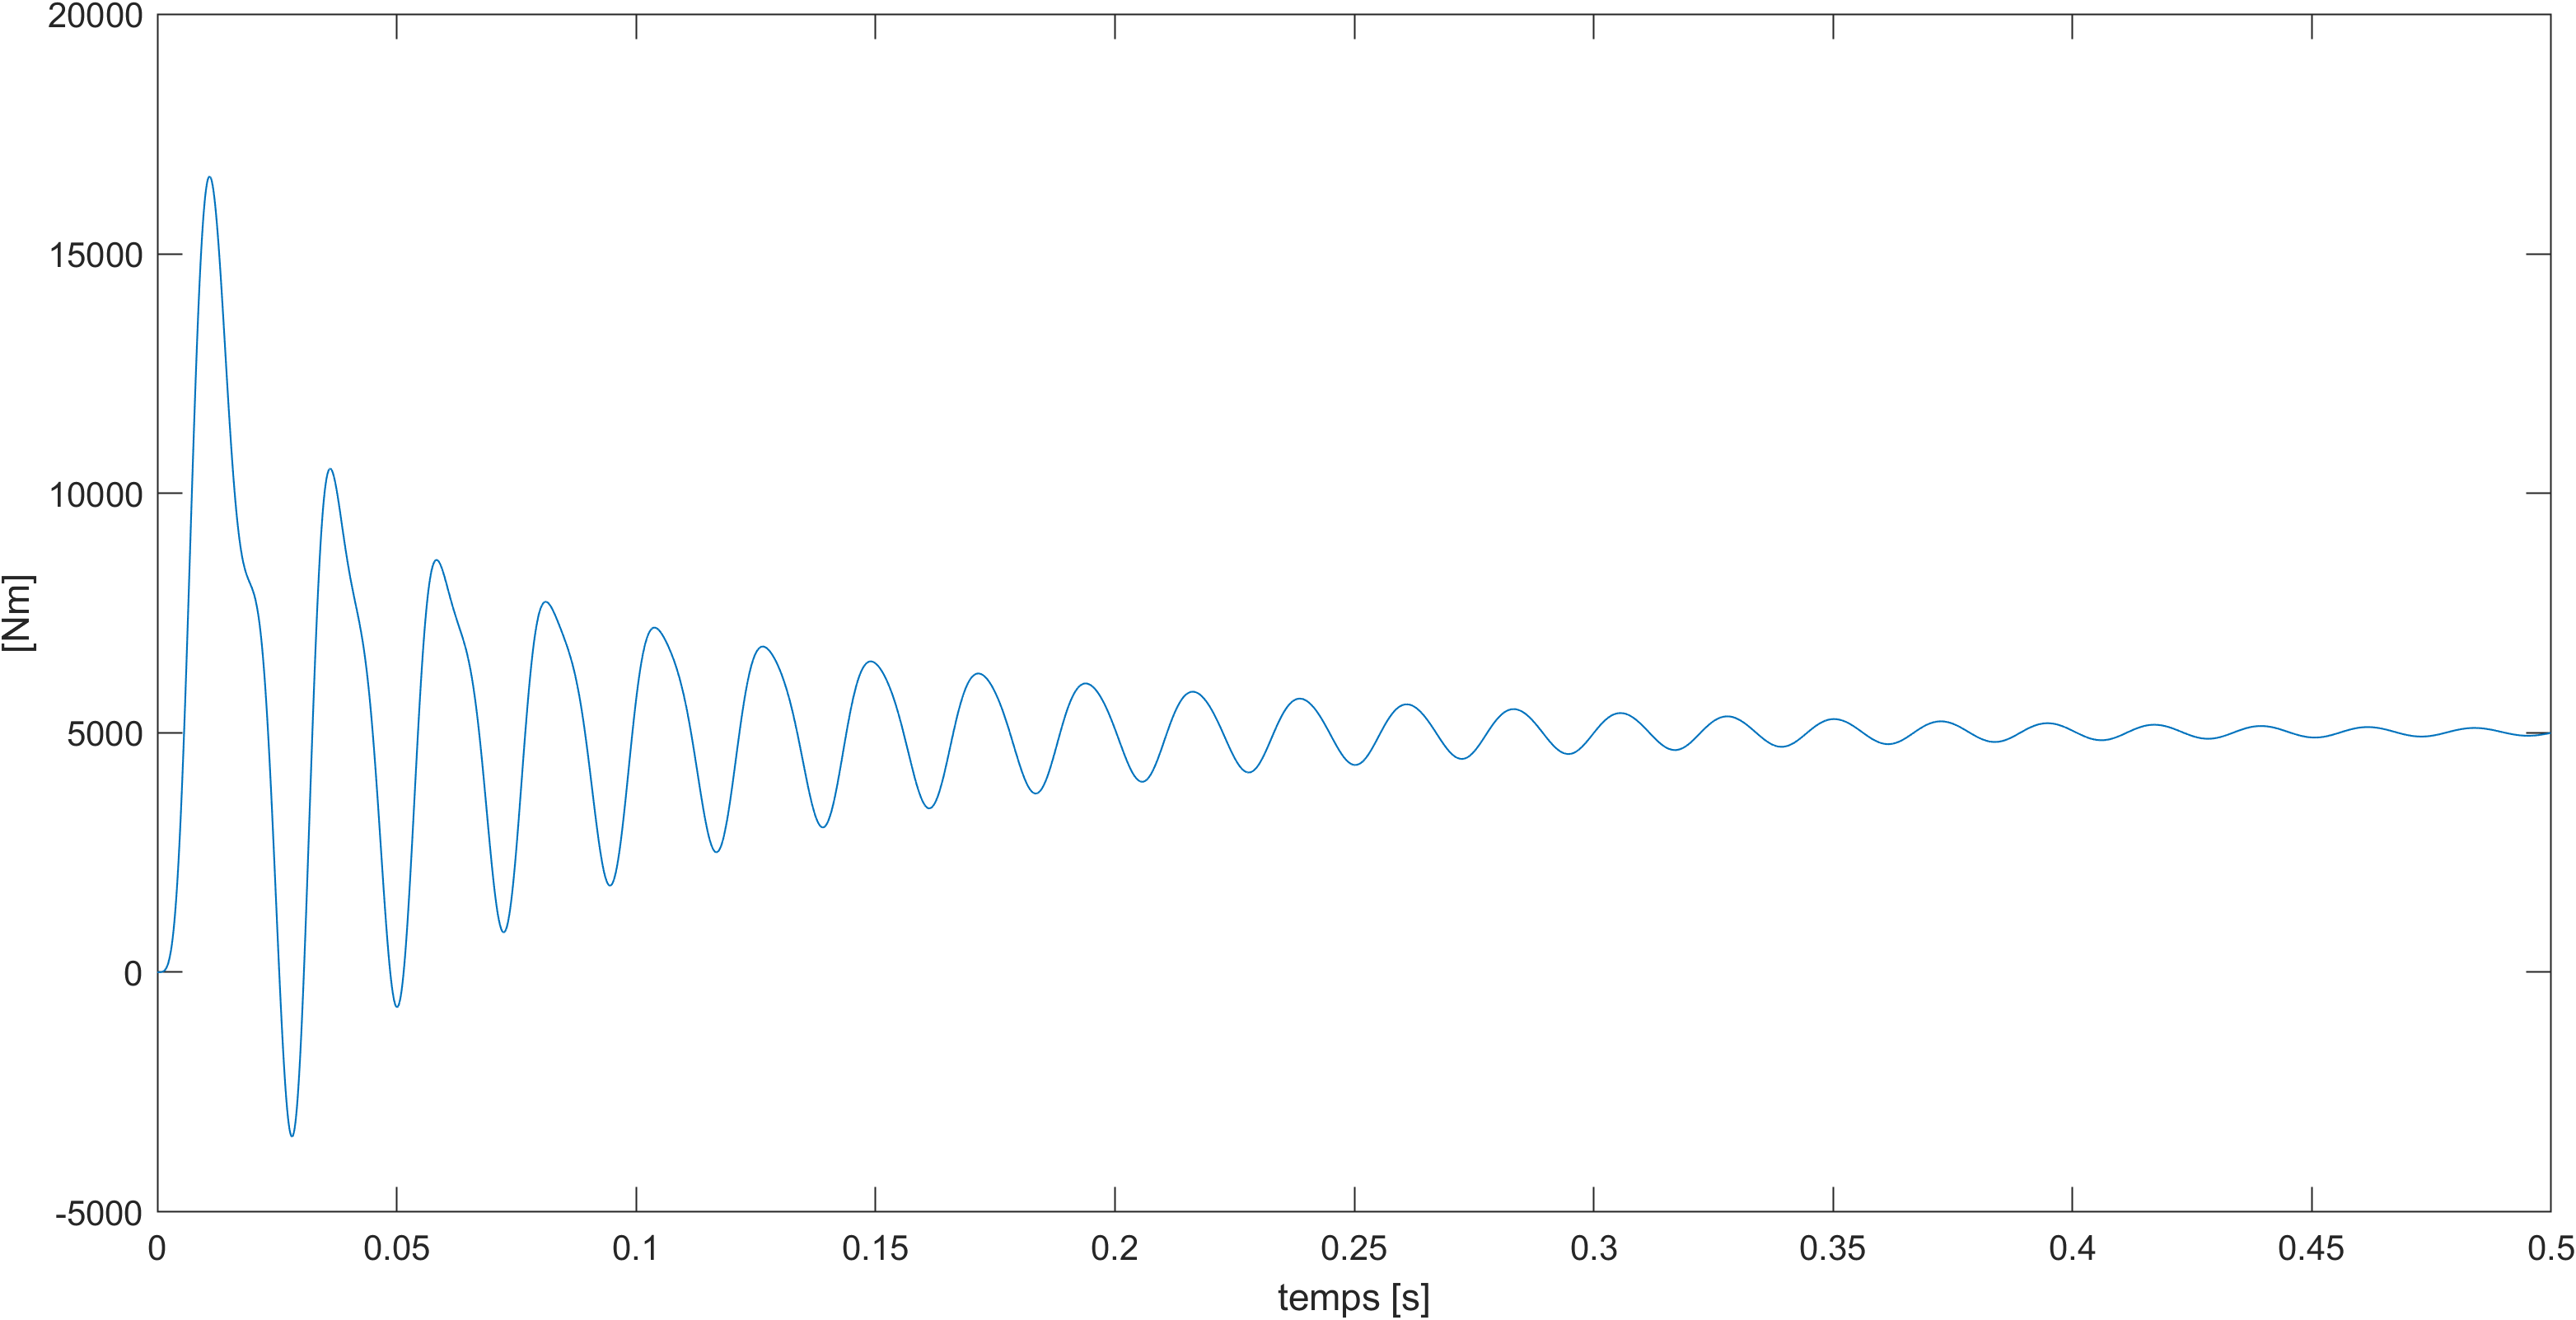
\includegraphics[width=0.8\textwidth]{simusMATLAB/MADA/Ce.png} 
    \caption{Couple de la MADA mesurée au cours du temps}
    \label{img-simuMADA-Ce}
\end{figure}


\begin{figure}[!h]
    \centering
    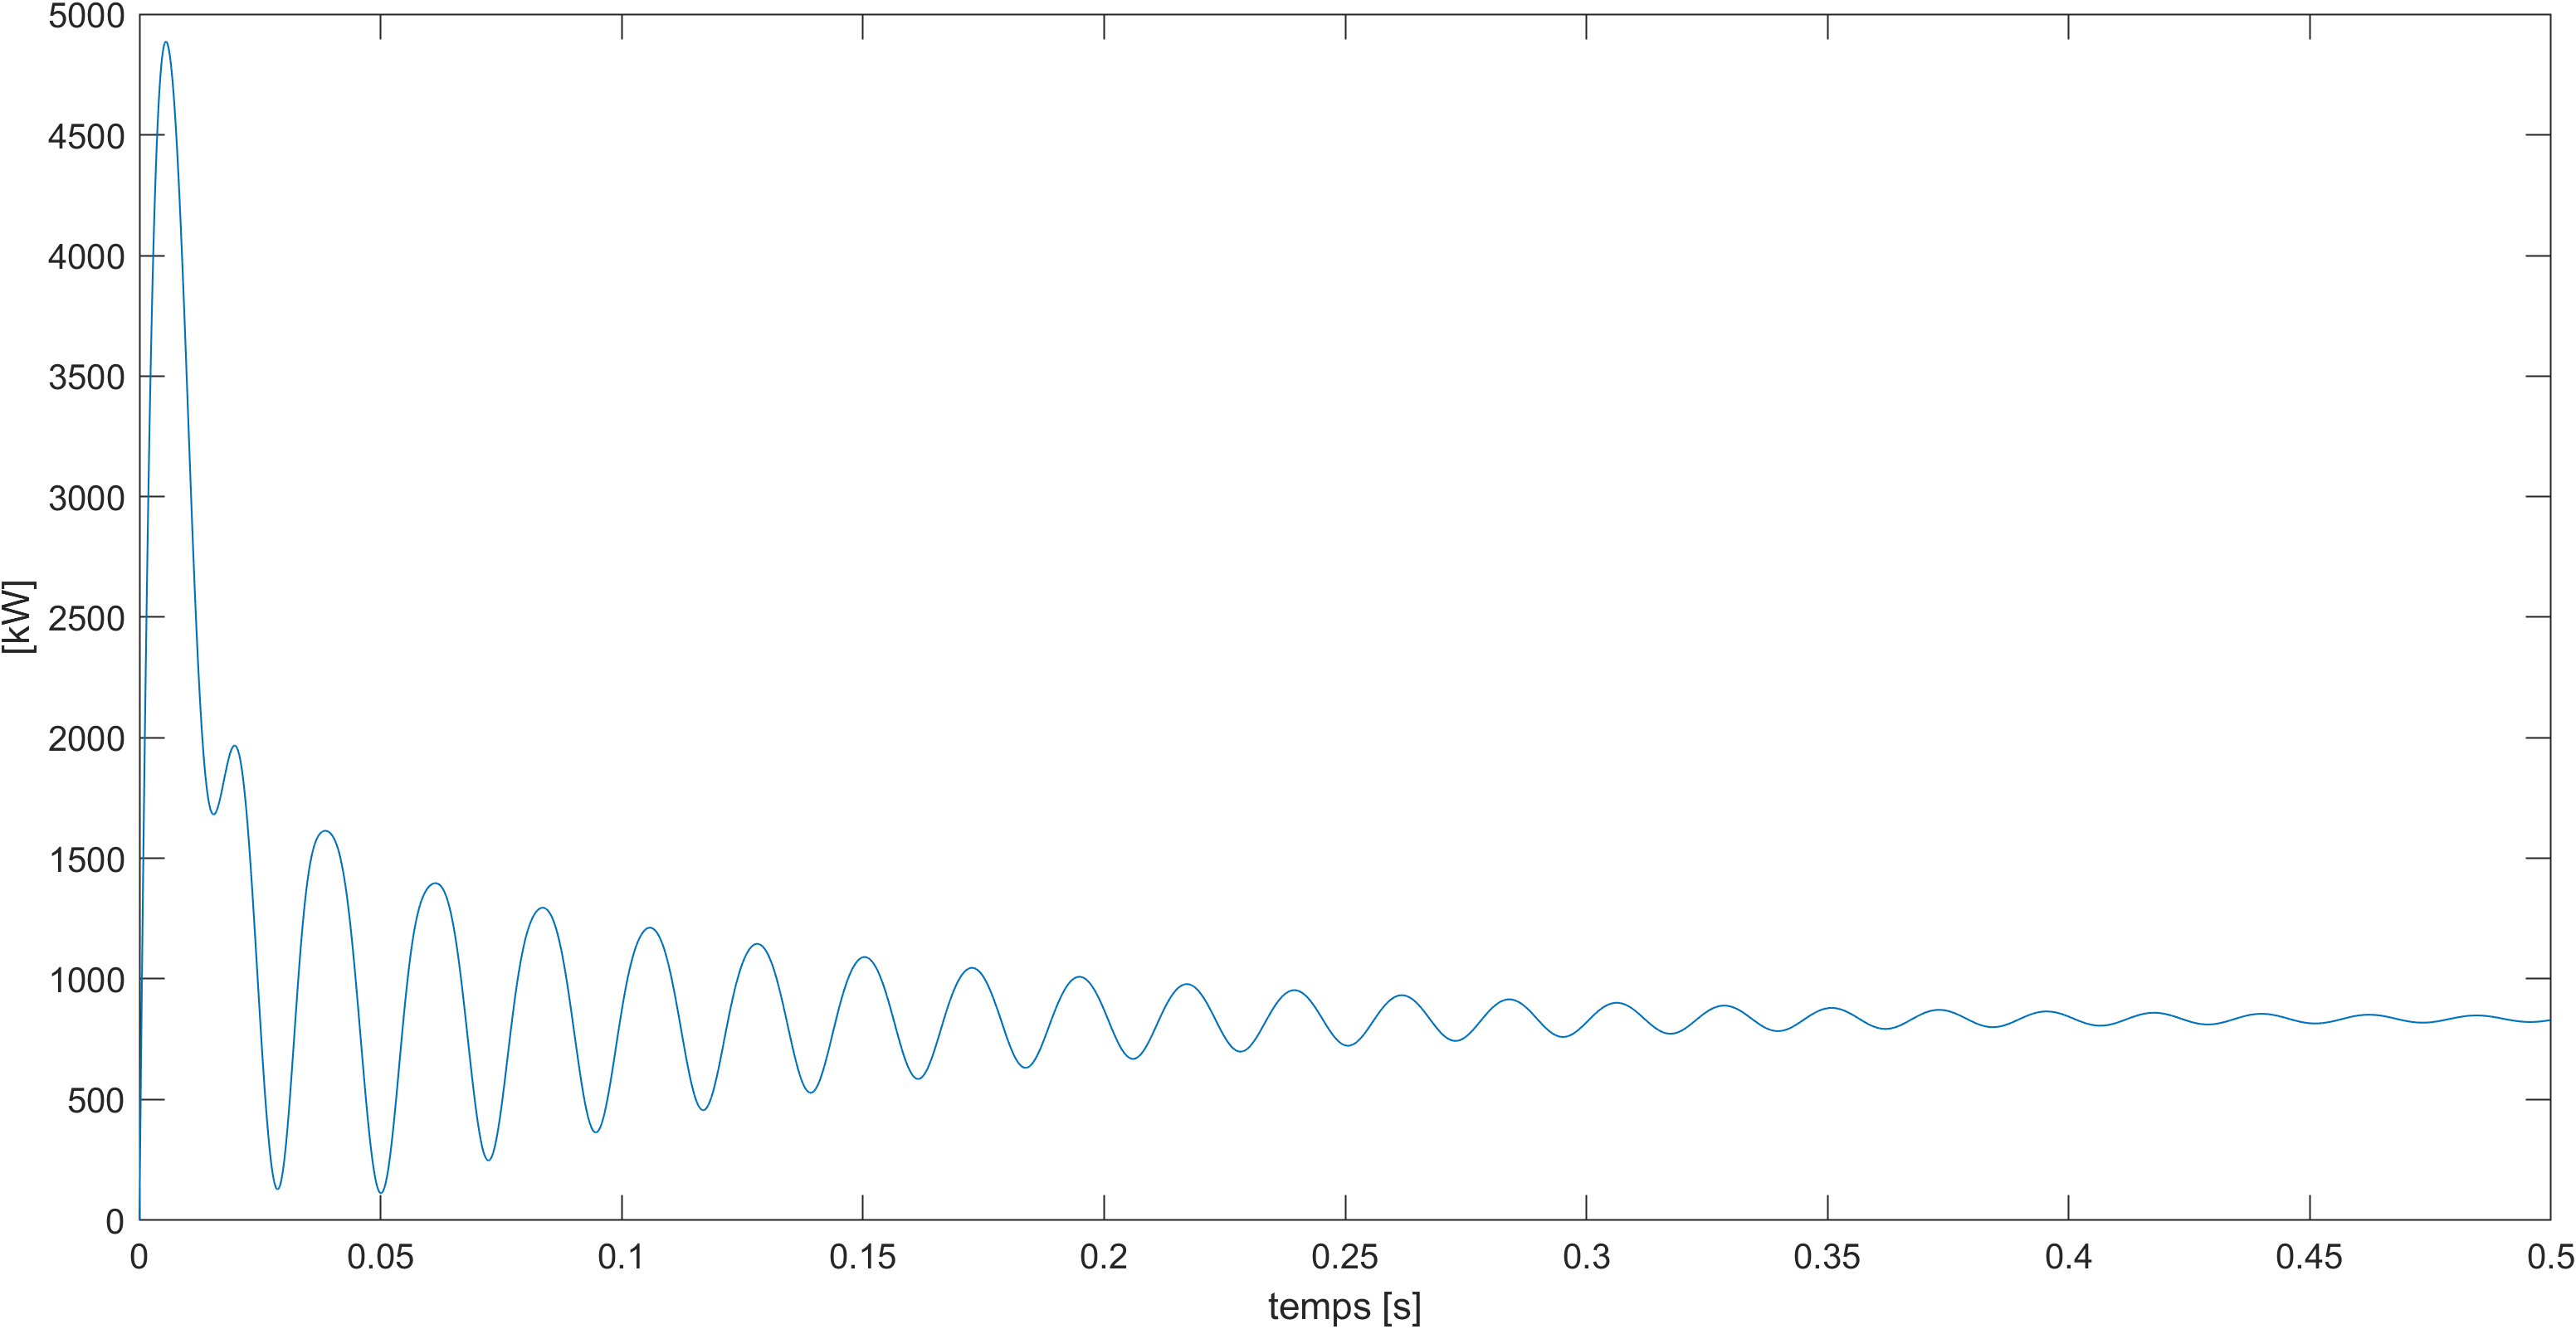
\includegraphics[width=0.8\textwidth]{simusMATLAB/MADA/P.png} 
    \caption{Courbe de la puissance de démarrage de la MADA.}
    \label{img-simuMADA-P}
\end{figure}


\begin{figure}[!h]
    \centering
    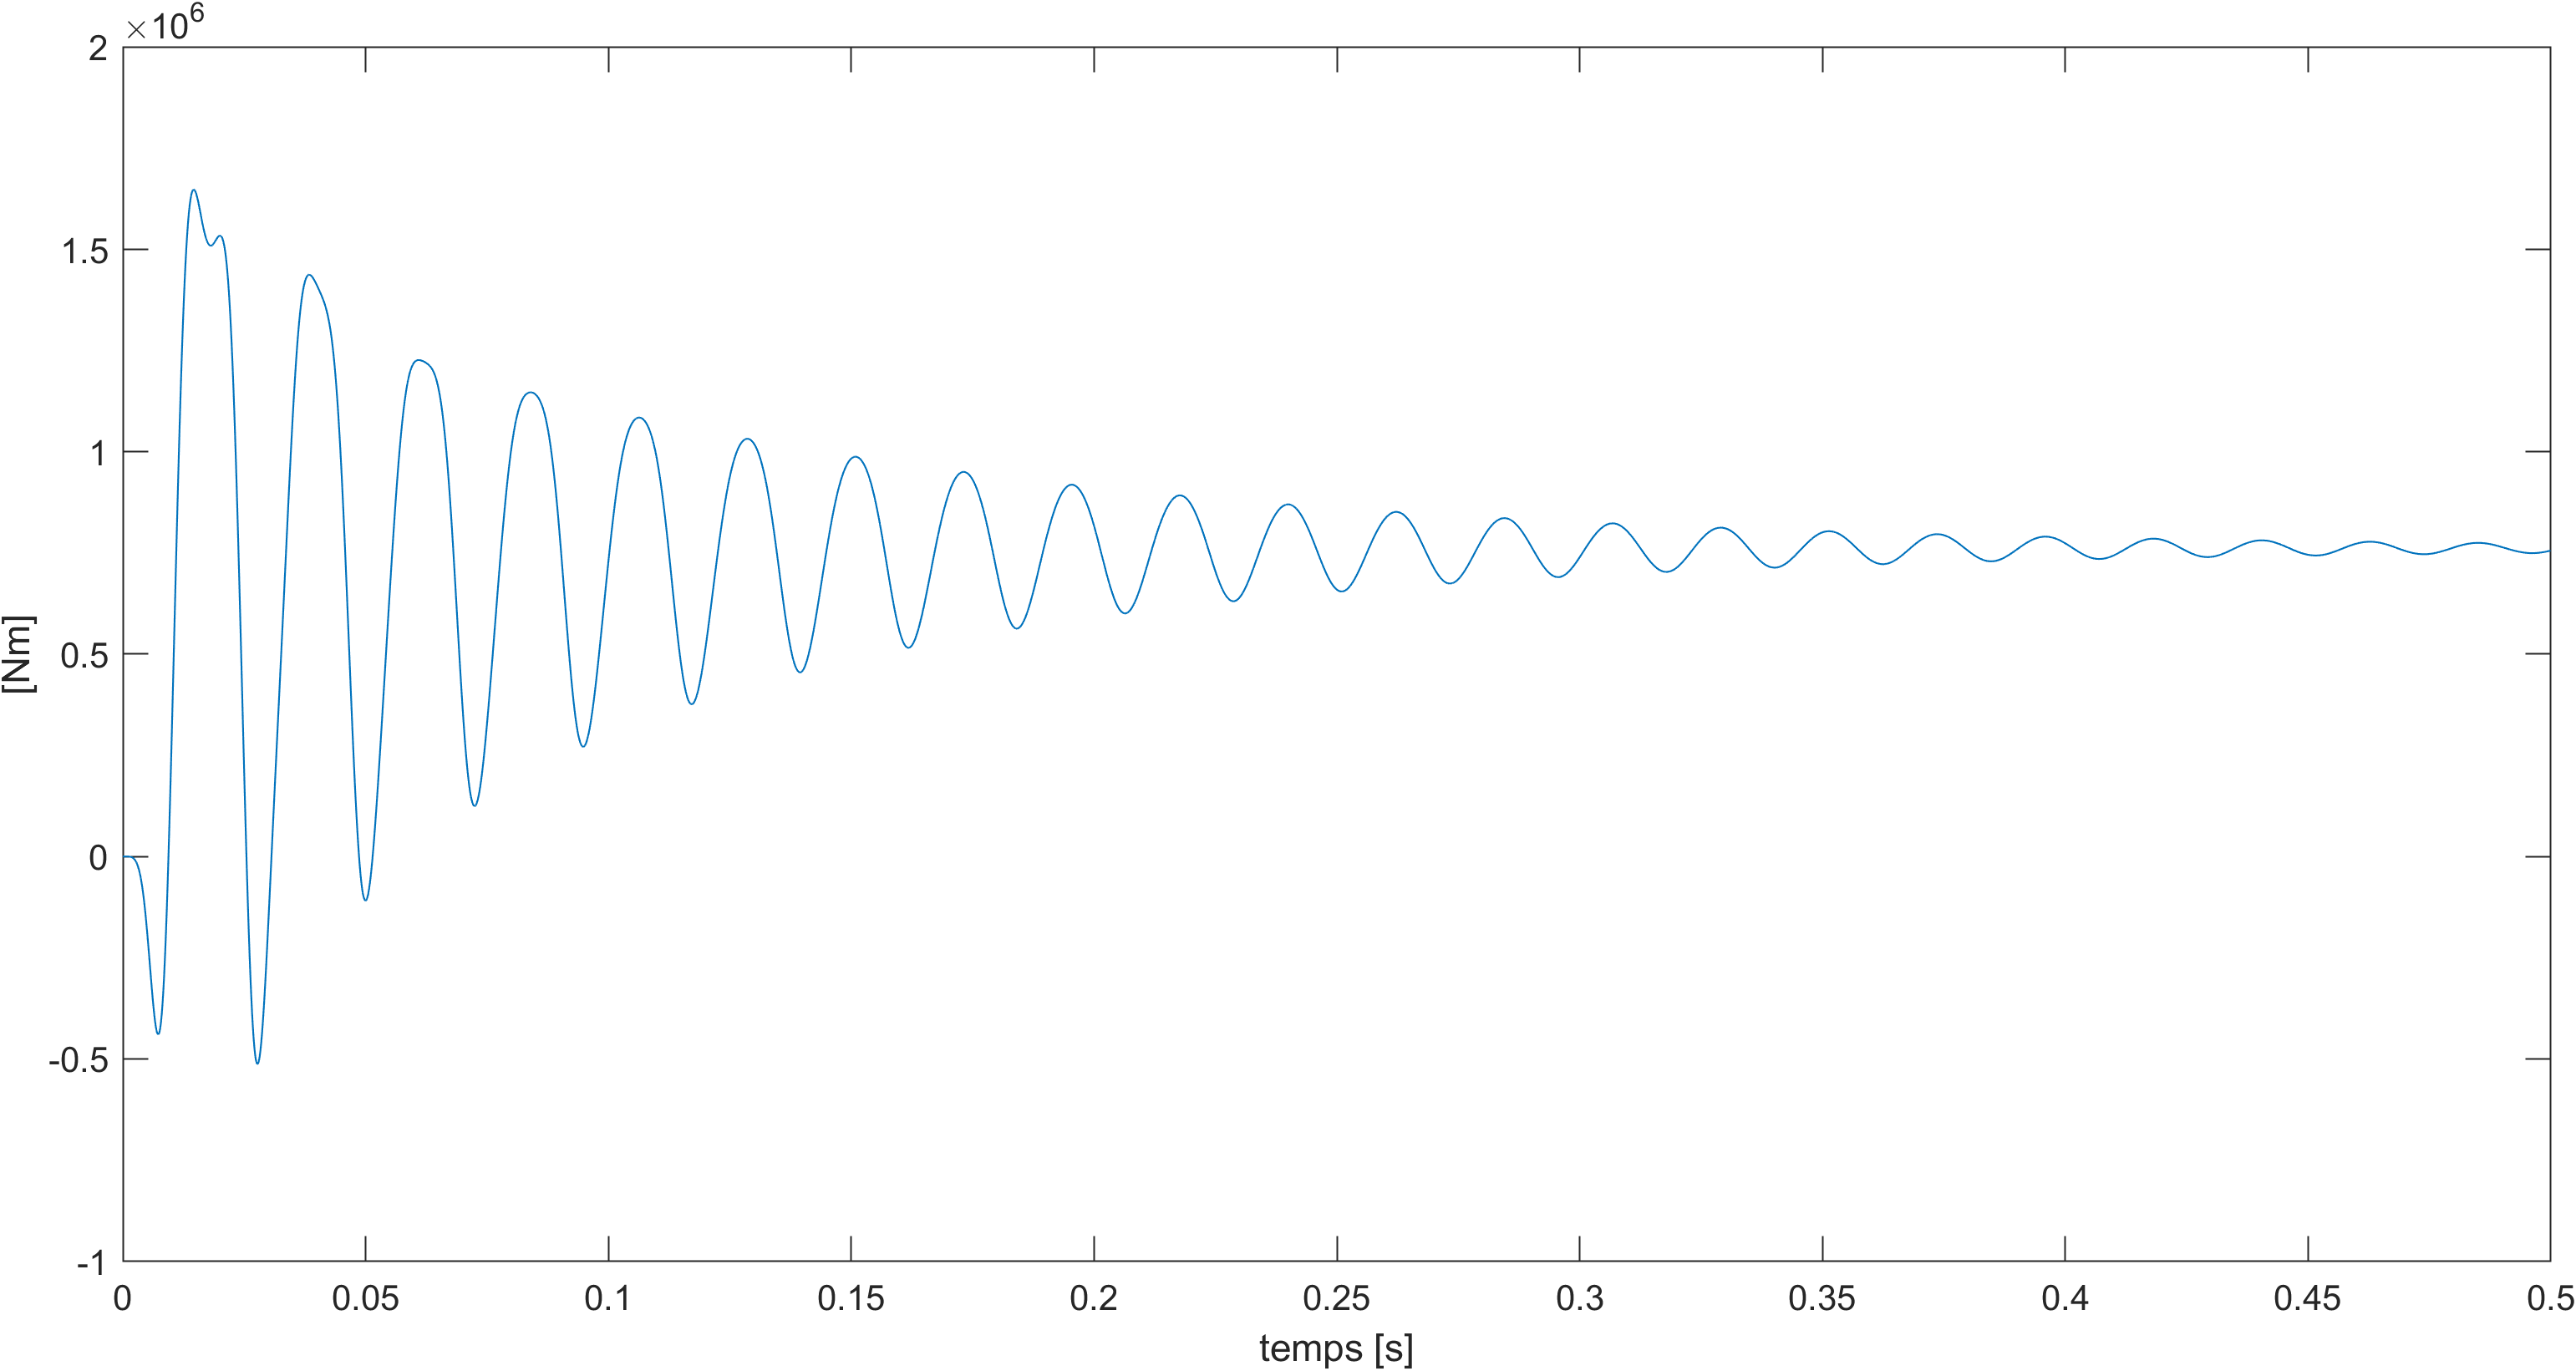
\includegraphics[width=0.8\textwidth]{simusMATLAB/MADA/torque.png} 
    \caption{Courbe du torque de démarrage de la MADA.}
    \label{img-simuMADA-torque}
\end{figure}


Après avoir simulé la MADA comme une machine à induction, plusieurs essais ont été effectués avec les contrôleurs de l'architecture présentée dans les figures \ref{img-diagMADA} et \ref{img-MADA}, mais sans résultats positifs. Pour le contrôleur, les coefficients $K_p$ et $\tau_i$ ont été calculés en utilisant la relation \ref{eq:MADA7} présentée. Ainsi, $K_p = 26,3158$ et $\tau_i = 0,0139$ ont été initialement calculés à l'aide de \ref{eq:MADA7} comme suit :


\begin{equation*}
    \left\{
    \begin{aligned}
        K_p =& \frac{1}{\alpha \cdot R_eq} \\
        \tau_i =& \beta \cdot \frac{L_eq}{R_eq}
    \end{aligned}
    \right. \;; \;\;
    \left\{
    \begin{aligned}
        L_{eq} =& L_r - \frac{M^2}{L_s} \\
        R_{eq} =& R_r
    \end{aligned}
    \right.
\end{equation*}

Simulink a présenté des erreurs de boucle algébrique dans plusieurs tentatives de simulation. Afin d'essayer de corriger l'erreur, le pas fixe du solveur Range-Kutta d'ordre 4 a été réduit, puis d'autres modèles de solveur disponibles dans Simulink ont été testés, ainsi que des modifications des paramètres de la machine et même des modifications de l'architecture du contrôleur, qui se sont toutes révélées infructueuses. En outre, pour tenter de corriger les erreurs de simulation, les contrôleurs autorégulateurs PI de Simulink ont été testés, mais ils n'ont pas non plus réussi à calculer les coefficients, affichant un message indiquant que le calcul divergeait et demandant de réduire le pas de simulation ou de changer de modèle. 

Parmi les architectures de contrôleurs autres que celles présentées ci-dessus qui ont été testées figurent les architectures présentées par BOYETTE \cite{Boyette2006}, illustrées dans les figures \ref{img-arc1}, \ref{img-arc2} et \ref{img-arc3}. Malheureusement, les erreurs du logiciel Simulink ont persisté et il n'a pas été possible d'extraire des données des simulations avec les contrôleurs de puissance MADA en fonctionnement.


\begin{figure}[!h]
    \centering
    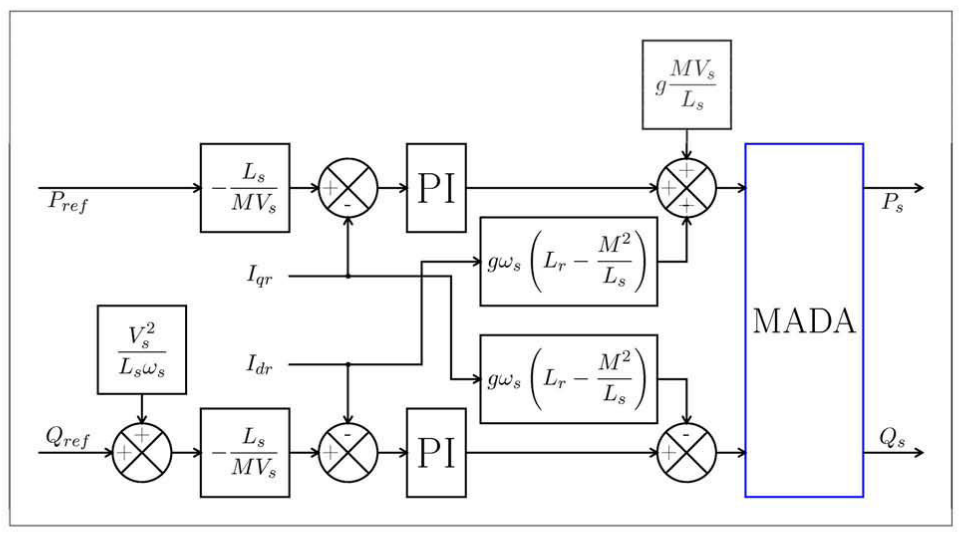
\includegraphics[width=0.8\textwidth]{diagrammes/arc1.png} 
    \caption{Schéma bloc de la commande indirecte \cite{Boyette2006}}
    \label{img-arc1}
\end{figure}

\begin{figure}[!h]
    \centering
    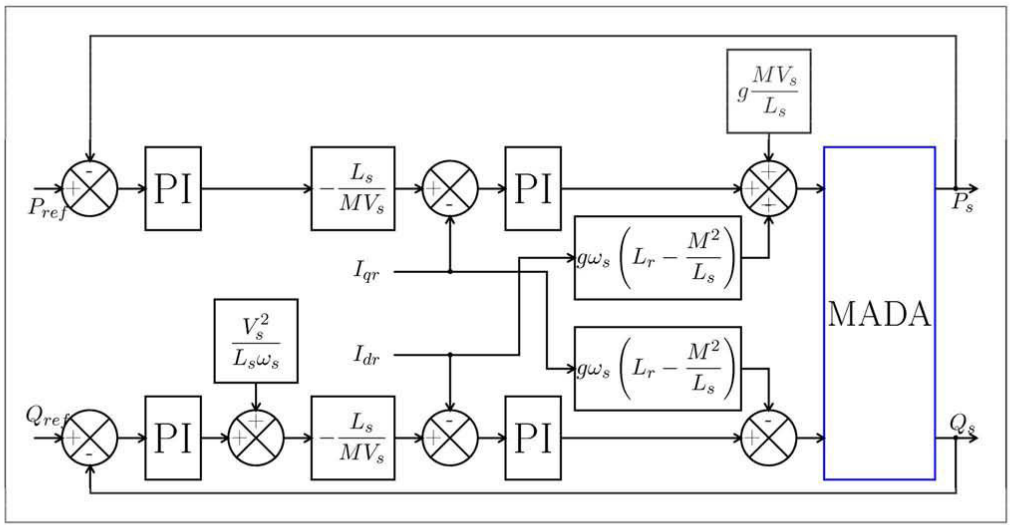
\includegraphics[width=0.8\textwidth]{diagrammes/arc2.png} 
    \caption{Schéma bloc de la commande indirecte avec boucles de puissance \cite{Boyette2006}.}
    \label{img-arc2}
\end{figure}

\begin{figure}[!h]
    \centering
    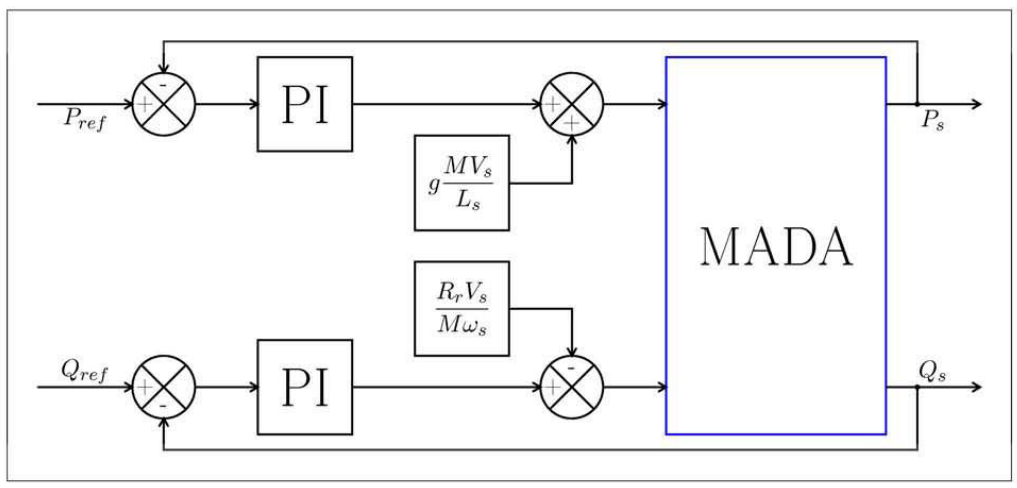
\includegraphics[width=0.8\textwidth]{diagrammes/arc3.png} 
    \caption{Schéma bloc de la commande directe \cite{Boyette2006}.}
    \label{img-arc3}
\end{figure}
